% Se compila con XeLaTeX; hacen falta varias pasadas para que se resuelvan las referencias.
\documentclass[11pt,a4paper]{article}
\usepackage{fontspec}
\IfFontExistsTF{texgyrepagella-regular.otf}
 {\setmainfont{texgyrepagella}[Extension=.otf,UprightFont=*-regular,BoldFont=*-bold,
   ItalicFont=*-italic,BoldItalicFont=*-bolditalic]}
 {\IfFontExistsTF{Palatino Linotype}{\setmainfont{Palatino Linotype}}{\setmainfont{Latin Modern Roman}}}
\linespread{1.05}
% Con babel-spanish instalado (MiKTeX, TeX Live completo) se usa la opción clásica; si falta,
% se carga el locale español de babel sin patrones de guionado y los cortes de palabra se
% toman de guionado.tex.
\IfFileExists{spanish.ldf}
 {\usepackage[spanish,es-noshorthands,es-nodecimaldot,es-tabla]{babel}}
 {\usepackage{babel}\babelprovide[import,main,hyphenrules=nohyphenation]{spanish}% Puntos de corte de las palabras del artículo según la división silábica de la Ortografía de
% la lengua española (RAE y ASALE, 2010); no se separan vocales contiguas. Sólo se usa cuando
% la instalación de TeX no trae los patrones de guionado del español (véase preambulo.tex).
\babelhyphenation[spanish]{
ab-so-lu-ta ab-so-lu-tas ab-so-lu-to ab-sor-be ab-sor-bien-do ab-sor-ción aba-jo abier-ta abier-to abs-ci-sa
ac-ción ac-ti-vas ac-ti-vi-da-des ac-ti-vi-dad ac-ti-vo ac-túa acer-can aco-pla-mien-to aco-ta aco-ta-da
aco-ta-do aco-ta-dos aco-ta-ron aco-tan aco-tar acom-pa-ña ad-jun-ta ad-jun-tos ad-mi-si-ble ad-mi-si-bles
ad-mi-te ad-mi-ten ad-ver-sa-ria-les adap-ta-ción ade-lan-te ade-más adi-cio-na-les adi-cio-nal afec-tan
afir-ma afir-ma-cio-nes afir-ma-ción aho-ra ais-la-da-men-te ajus-te ajus-tes al-can-ce al-can-za
al-ge-brai-cas al-ge-brai-cos al-go-rit-mo al-gu-na al-gu-nas al-re-de-dor al-te-ra ale-ja-do alea-to-rias
am-bas am-bi-güe-dad am-bos an-chu-ra an-te-rio-res an-te-rior an-tes an-ti-dia-go-na-les an-ti-dia-go-nal
an-ti-si-mé-tri-co ano-ta-mos anu-la anu-lan anun-cia-da aná-lo-ga aná-lo-ga-men-te aná-lo-go apa-re-ce
apa-re-cen apar-ta apar-te apli-ca apli-ca-ción apli-ca-da apli-ca-do apli-ca-mos apli-can apli-can-do
apli-car apo-ya apor-ta apor-ta-ción apor-tan apro-xi-ma apro-xi-ma-cio-nes apro-xi-ma-ción
apro-xi-ma-da-men-te apro-xi-ma-do apro-xi-mar apén-di-ce ar-bi-tra-rias ar-bi-tra-rios ar-gu-men-to
ar-gu-men-tos ar-ti-fi-cial ar-tí-cu-lo aris-ta aris-tas arit-mé-ti-ca arri-ba ase-gu-rar asi-mis-mo asig-na
asig-na-da asig-na-dos asin-tó-ti-ca asin-tó-ti-co asin-tó-ti-cos aso-cia-das ata-ca-das ata-can ata-quen
ata-ques au-men-tar au-to-va-lo-res au-to-va-lor au-toad-jun-ta au-toad-jun-to au-toad-jun-tos au-xi-lia-res
aña-de aña-den aña-dien-do aña-dir ba-lan-ce ba-rre-ra ban-das bas-ta bas-tan bi-di-men-sio-nal bi-no-mial
bi-par-ti-to bi-yec-ción blo-que blo-ques bo-rrar bre-cha ca-nó-ni-ca ca-nó-ni-co ca-re-cen ca-si-lla
ca-si-llas ca-sos cal-cu-la cal-cu-la-do cal-cu-la-mos cal-cu-lan cal-cu-lar cam-bia cam-bia-da cam-bian
cam-bio cam-bios cam-po cam-pos can-ce-la can-ce-la-ción can-ce-lan can-di-da-tas can-ti-da-des can-ti-dad
car-di-na-li-da-des car-lo ce-ros ce-rra-das ce-rra-dos cel-da cel-das cen-tra-dos cen-tro cer-ca cer-ca-no
cer-ca-nía cer-ti-fi-ca-da ci-fras ci-ta-do cie-rre cin-co cla-se cla-ses cla-ve co-cien-te co-fac-to-res
co-fac-tor co-las co-lo-ca co-lo-ca-cio-nes co-lo-ca-ción co-lo-ca-das co-lo-car co-lo-res co-lum-na
co-lum-nas co-ne-xo co-ne-xos co-nec-ti-vi-dad co-no-cen co-no-ci-do co-ro-la-rio co-ro-nas co-rre-gi-da
co-rre-gir co-rrec-cio-nes co-rrec-ción co-rres-pon-de co-rres-pon-den co-rres-pon-den-cia
co-rres-pon-dien-te co-se-nos co-tas co-te-jar co-vo-lu-men coe-fi-cien-te coe-fi-cien-tes coer-ci-vi-dad
coin-ci-da coin-ci-de coin-ci-den com-bi-na com-bi-na-ción com-bi-nan com-bi-nar com-pa-ci-dad com-pa-ra
com-pa-ra-ción com-pa-ra-mos com-pa-ran com-pa-rar com-pa-ti-bi-li-dad com-pa-ti-ble com-pa-ti-bles
com-pac-to com-par-ten com-pen-sa com-pen-se com-ple-men-ta-rie-dad com-ple-men-to com-ple-men-tos
com-ple-ta com-ple-ta-bi-li-dad com-ple-ta-cio-nes com-ple-ta-ción com-ple-tar-se com-ple-tas com-ple-to
com-po-nen-te com-po-nen-tes com-po-si-ción com-pro-ba-do com-pro-bar-lo com-prue-ba con-ca-vi-dad
con-cen-tra con-clu-sión con-clui-mos con-di-cio-na-da con-di-cio-nes con-di-ción con-fir-mó con-je-tu-ra
con-jun-tos con-se-cuen-cia con-se-cuen-cias con-ser-va con-ser-va-ción con-ser-va-mos con-ser-van
con-ser-van-do con-ser-var con-si-de-ra con-si-de-ra-mos con-si-de-ran-do con-si-go con-sis-te
con-sis-ten-cia con-ta-bi-li-dad con-ta-do con-tan-do con-tar con-tar-las con-teo con-teos con-tex-to
con-ti-nua con-ti-nua-ción con-ti-nuas con-ti-nui-dad con-ti-nuo con-ti-nuos con-tie-ne con-tra
con-tra-di-ce con-tra-rio con-trac-ti-va con-tras-ta con-tri-bu-cio-nes con-tri-bu-ción con-tri-bu-ye
con-tri-bu-yen con-tro-la con-tro-lan con-tro-lar con-tro-les con-trol con-ve-xa con-ve-xi-dad con-ve-xo
con-ven-cio-nes con-ven-ción con-ver-ge con-ver-gen con-ver-gen-cia con-ver-gen-tes con-vie-ne con-vier-te
cons-tan-tes cons-tru-ye cons-tru-yen cons-truc-ción cons-trui-do cons-trui-mos cons-truir coor-de-na-da
coor-de-na-das cor-che-te cor-ta cor-tan cor-tar-se cor-tas cre-ce cre-cien-te cru-ces cru-za-dos crí-ti-co
cu-yos cua-dra-do cua-dra-dos cua-dra-tu-ra cua-drá-ti-ca cua-drá-ti-co cua-drá-ti-cos cua-sia-lea-to-rios
cua-tro cual-quie-ra cual-quier cuan-do cuan-ti-ta-ti-va cuan-ti-ta-ti-vas cuan-to cuar-ta cuen-ta cuer-da
cues-ta cues-tión cum-pla cum-plan cum-ple cum-plen cum-plie-ra cur-va-tu-ra cuá-les cuán-ta cuán-tas
cuán-to cál-cu-lo cál-cu-los cír-cu-los cón-ca-va cón-ca-vo cú-bi-co cú-bi-cos da-tos de-ci-mos de-cir
de-cla-ra-da de-cre-ce de-cre-cien-te de-du-ce de-fec-to de-fec-tos de-fi-ne de-fi-nen de-fi-ni-cio-nes
de-fi-ni-ción de-fi-ni-da de-fi-ni-das de-fi-ni-do de-fi-ni-dos de-fi-ni-mos de-ge-ne-ra-do de-jan
de-li-mi-tan de-mos-tra-ción de-mos-tra-da de-mos-tra-do de-mues-tra de-más de-no-ta de-no-ta-da
de-no-ta-mos de-pen-de de-pen-den de-pen-den-cias de-pen-dien-tes de-re-cha de-ri-va-ción de-ri-va-da
de-ri-va-das de-ri-va-ti-va de-ri-var de-sa-pa-re-ce de-sa-pa-re-cen de-sa-rro-lla de-sa-rro-llan
de-sa-rro-llo de-sa-rro-llos de-se-chan de-si-gual-da-des de-si-gual-dad de-sig-na de-sig-nan de-ter-mi-na
de-ter-mi-na-do de-ter-mi-nan-te de-ter-mi-nan-tes de-ter-mi-nis-ta de-ter-mi-nis-tas de-ter-mi-nó den-sa
den-si-da-des den-si-dad den-so den-tro des-car-tar-se des-com-po-si-ción des-cri-ben des-de
des-fa-vo-ra-bles des-pa-cio des-pe-jar des-pla-za-mien-to des-pre-cia-ble des-pués di-fe-ren-cia
di-fe-ren-cia-ble di-fe-ren-cia-bles di-fe-ren-cial di-fie-re di-fie-ren di-men-sio-nes di-men-sión
di-rec-ción di-rec-ta di-rec-ta-men-te di-vi-de di-vi-den di-vi-di-da di-vi-di-do di-vi-di-mos di-vi-dien-do
di-vi-dir dia-go-na-les dia-go-nal die-ron dis-con-ti-nua dis-cre-ta dis-cre-tas dis-cre-ti-za-ción
dis-cre-to dis-cre-tos dis-cu-sión dis-per-sa dis-po-ni-ble dis-po-ni-bles dis-tan-cia dis-tin-gue
dis-tin-ta dis-tin-tas dis-tin-to dis-tin-tos do-ble do-ble-men-te do-mi-na-da do-mi-na-do do-mi-nio don-de
dé-bi-les dé-bil dé-fi-cits dón-de ecua-cio-nes ecua-ción edi-to-rial efec-ti-va efec-to ejem-plo ele-gi-da
ele-gi-das ele-gi-mos ele-gir elec-cio-nes elec-ción eli-ge eli-gen eli-mi-na eli-mi-na-ción eli-mi-na-da
eli-mi-na-das eli-mi-na-do eli-mi-na-dos eli-mi-nan eli-mi-nar-se eli-mi-nán-do-las em-pa-re-ja-mien-tos
em-pe-zan-do em-pie-zan en-cuen-tra en-sa-ya-das en-te-ro en-ten-der en-ton-ces en-tra-da en-tra-das en-tran
en-tre en-tre-la-za-dos en-tro-pía en-tro-pías en-tró-pi-ca ener-gía enu-me-ra-ción enun-cia-do enun-cia-dos
equi-va-le equi-va-len-te erro-res es-ca-la es-ca-la-res es-ca-lar es-ca-lo-na-dos es-co-ge es-co-ge-mos
es-cri-ba-mos es-cri-be es-cri-ben es-cri-bi-mos es-cri-bien-do es-cri-bir es-cri-ta es-cri-to es-pa-cia-das
es-pa-cial es-pa-cio es-pe-ci-fi-ca es-pec-tral es-pec-tro es-ta-ble-ce es-ta-ble-cen es-ta-cio-na-ria
es-ta-cio-na-rias es-ta-cio-na-rie-dad es-ta-cio-na-rio es-ta-dos es-tar es-tas es-ti-ma-cio-nes
es-ti-ma-ción es-ti-mar es-to-cás-ti-ca es-tos es-tre-cha es-tric-ta es-tric-ta-men-te es-tric-to
es-truc-tu-ra es-tu-dia es-tu-dia-do es-tu-dia-mos es-tu-dia-ron es-tu-dian es-tán es-tén esen-cial
eti-que-tas eu-clí-dea eu-clí-deas eu-clí-deo eva-lua-cio-nes eva-lua-ción eva-lua-da eva-luar eva-lúa
evi-den-cia evi-tar ex-cep-cio-nal ex-clu-si-va-men-te ex-clu-ye ex-clu-yen ex-hi-bi-mos ex-pan-de
ex-pan-dir ex-pan-sio-nes ex-pan-sión ex-pli-ca ex-plí-ci-ta ex-plí-ci-tas ex-plí-ci-to ex-po-nen-cia-les
ex-po-nen-cial ex-pre-sa ex-pre-san ex-pre-sio-nes ex-pre-sión ex-pues-to ex-te-rior ex-ten-da-mos
ex-ten-de-mos ex-ten-der ex-ten-sión ex-tien-de ex-tra-po-la-cio-nes ex-tra-po-la-ción ex-trac-tos ex-tre-mo
ex-tre-mos exac-ta exac-ta-men-te exac-tas exac-to exac-tos exi-ge exi-gi-ría exi-gir exis-ta exis-te
exis-ten exis-ten-cia exis-ti-ría exis-tir fa-lla-ra fa-mi-lia fa-mi-lias fac-ti-bi-li-dad fac-ti-ble
fac-to-res fac-to-ri-za fac-to-ri-za-ción fac-tor fal-ta fal-tan fi-bra fi-bras fi-gu-ra fi-ja-ción fi-ja-da
fi-ja-das fi-ja-do fi-ja-mos fi-jar fi-jas fi-je-mos fi-jos fi-las fi-nal fi-nal-men-te fi-ni-ta fi-ni-to
fi-ni-tos fle-cha flo-tan-te for-ma for-ma-da for-man for-mas for-mu-la-ción for-mu-lar frac-cio-na-rias
frac-cio-nes frac-ción fron-te-ra fue-ra fuen-te fuen-tes fun-cio-nal fun-cio-nes fun-ción fun-da-men-tal
fí-si-ca fór-mu-la fór-mu-las gat-he-red gau-ge gau-ges gaus-sia-na ge-ne-ra-da ge-ne-ra-tri-ces
ge-ne-ra-triz ge-ne-ral geo-me-tría geo-mé-tri-ca-men-te geo-mé-tri-cas glo-bal gra-dien-te gra-do gra-fo
gra-fos gran-de ha-ber ha-bría ha-bía ha-ce-mos ha-cen ha-cia has-ta he-cho he-mos he-re-da-da he-ren-cia
he-rra-mien-tas hes-sia-na heu-rís-ti-ca-men-te heu-rís-ti-co hi-jos hi-pó-te-sis his-to-ria ho-jas
ho-ri-zon-tal iden-ti-da-des iden-ti-dad iden-ti-fi-ca iden-ti-fi-ca-ción iden-ti-fi-ca-do iden-ti-fi-can
iden-ti-fi-car idén-ti-ca-men-te igua-les igual-da-des igual-dad igual-men-te im-pa-res im-par im-pi-den
im-ple-men-ta-ción im-pli-ca im-pli-can im-plí-ci-ta im-po-ne ima-gen in-ci-den-cia in-ci-den-cias
in-cli-na-da in-clu-so in-clu-ye in-clu-yen in-clui-do in-clui-dos in-clui-mos in-cluir in-cor-po-ra
in-cor-po-ra-do in-cor-po-ró in-cre-men-to in-cre-men-tos in-cóg-ni-ta in-cóg-ni-tas in-de-pen-den-cia
in-de-pen-dien-te in-de-pen-dien-tes in-de-xa-da in-de-xa-do in-de-xa-dos in-di-ca in-di-ca-do-res
in-di-ca-dor in-di-ca-mos in-di-que in-fe-rior in-fi-ni-ta in-fi-ni-to in-for-ma-ción in-for-ma-ti-vo
in-gre-dien-tes in-ser-cio-nes in-ser-ción in-ser-ta-da in-ser-tar in-tac-tas in-te-gra in-te-gra-les
in-te-gral in-te-gran-dos in-te-grar in-te-li-gen-cia in-te-rio-ri-dad in-te-rior in-ter-me-dios
in-ter-po-la in-ter-po-lan in-ter-pre-ta-ción in-ter-sec-cio-nes in-ter-sec-ción in-ter-va-lo in-ter-va-los
in-ter-vie-ne in-ter-vie-nen in-tro-du-ci-mos in-tro-du-cir in-tro-duc-ción in-trín-se-ca in-va-rian-te
in-va-rian-tes in-ver-sa in-ver-sas in-ver-so in-ver-ti-ble in-vo-ca ini-cial iso-me-tría iso-me-trías
ite-ra ite-rar iz-quier-da iz-quier-do ja-co-bia-na jun-to ka-rush la-bel la-dos la-pla-cia-no la-te-ra-les
la-ti-nos la-zos lar-go le-ga-les le-gal le-ma-sub le-mas le-tra le-tras le-van-ta-mien-to lec-tu-ra lee-mos
li-nea-les li-neal lis-ta lla-ma-mos lle-gar lle-no lle-va lle-van lle-ve lo-cal lo-ga-rit-mo lo-ga-rit-mos
lo-ga-rít-mi-ca lo-ga-rít-mi-ca-men-te lon-gi-tud lu-gar lue-go lí-mi-te lí-mi-tes lí-nea lí-neas
ma-cros-có-pi-ca ma-lla ma-llas ma-ne-ra ma-ne-ras ma-sas ma-tri-ces ma-tri-cial ma-triz ma-xi-ma-li-dad
ma-xi-mi-za ma-xi-mi-za-dor ma-xi-mi-zan ma-yor mag-ni-tu-des man-te-ne-mos man-te-ner-se man-te-nien-do
man-tie-ne man-tie-nen mar-ca mar-ca-das mar-gen mar-gi-na-les mar-gi-nal me-di-da me-di-das me-dia
me-dian-te me-dias me-dio me-dios me-no-res me-nor me-nos me-sos-có-pi-ca mi-ni-mi-za-dor mi-ni-mi-zar
mi-rar miem-bro miem-bros mien-tras mis-ma mis-mas mis-mo mis-mos mo-de-lo mo-de-los mo-men-tos mo-no-to-nía
mo-ti-va mon-te mu-chas mu-tuas mues-tra mues-tran mues-treo mul-ti-pli-ca mul-ti-pli-ca-da mul-ti-pli-ca-do
mul-ti-pli-ca-do-res mul-ti-pli-ca-dor mul-ti-pli-ca-mos mul-ti-pli-ca-ti-va mul-ti-pli-can-do
mul-ti-pli-car-se mul-ti-pli-ci-da-des mul-ti-pli-ci-dad má-xi-ma má-xi-mo már-ge-nes más-ca-ra mé-to-do
mó-du-lo múl-ti-plo múl-ti-plos na-tu-ral ne-ce-sa-ria-men-te ne-ce-sa-rias ne-ce-sa-rio ne-ce-si-ta
ne-ce-si-ta-mos ne-ga-ti-va ne-ga-ti-vas ne-ga-ti-vo ne-ga-ti-vos neu-tro nin-gu-na nin-gu-no nin-gún
no-cio-nes no-dos no-ta-cio-nes no-ta-ción no-viem-bre nor-ma nor-ma-les nor-ma-li-za-cio-nes
nor-ma-li-za-ción nor-ma-li-zar nor-mal nor-mas nu-las nu-los nu-me-ra-dos nu-me-ra-mos nu-me-ran
nu-mé-ri-ca nu-mé-ri-ca-men-te nu-mé-ri-co nue-va nue-vas nue-vo nun-ca nú-cleo nú-cleos nú-me-ro nú-me-ros
ob-je-ti-vo ob-je-to ob-je-tos ob-ser-va-ción ob-sér-ve-se ob-te-ne-mos ob-te-ner ob-te-ner-se ob-te-ni-do
ob-tie-ne ob-tie-nen ob-tu-vie-ron obli-ga ocu-pa-ción ocu-pa-das ocu-par ocu-rre ofre-ce ol-vi-dar omi-sión
omi-ten omi-ti-mos omi-tien-do omi-tir omi-tió op-cio-nes op-ti-ma-li-dad op-ti-mi-za-dor ope-ra-cio-nes
ope-ra-ción ope-ra-do-res ope-ra-dor opues-tas opues-to or-de-na-dos or-de-na-mos or-den or-di-na-rias
or-di-na-rio or-ga-ni-za-ción or-ga-ni-zar or-to-go-na-les or-to-go-nal or-to-nor-mal ori-gen ori-gi-na-les
ori-gi-nal orien-ta-ción orien-ta-das os-ci-la-cio-nes os-ci-la-to-rios pa-dre pa-dres pa-la-bras
pa-no-ra-ma pa-pel pa-que-te pa-ra-le-la pa-ra-mé-tri-ca pa-re-jas pa-ren-tal pa-rent pa-res pa-ri-da-des
pa-ri-dad pa-rá-me-tro pa-rá-me-tros pa-san pa-sar pa-sos par-cial par-te par-tes par-ti-ción par-ti-cu-lar
par-ti-da par-tir pe-que-ña pe-que-ño pe-que-ños pe-rió-di-co pe-sos pen-dien-te per-de-ría per-fec-tos
per-fi-les per-ju-di-ca per-ma-ne-ce per-ma-ne-cen per-ma-nen-cia per-ma-nen-te per-ma-nen-tes per-ma-nez-ca
per-ma-nez-can per-mi-ta-mos per-mi-te per-mi-ten per-mu-ta-cio-nes per-mu-ta-ción per-mu-to-nes
per-pen-di-cu-lar per-sis-te per-te-ne-ce per-te-ne-cen per-te-nen-cia per-te-nez-ca per-tur-ba-ción
per-tur-ba-dor pi-vo-te pie-zas pier-de pma-trix po-cas po-de-mos po-li-no-mio po-li-no-mios po-li-to-po
po-los po-ne-mos po-ner po-nien-do po-si-bi-li-da-des po-si-bles po-si-ti-va po-si-ti-vas po-si-ti-vi-dad
po-si-ti-vo po-si-ti-vos po-ten-cia-les po-ten-cial po-ten-cial-men-te po-ten-cias pon-de-ra-da pon-de-ra-do
pon-ga-mos por-que pre-ci-san pre-ci-sión pre-ci-so pre-dic-cio-nes pre-dic-ción pre-fac-tor pre-gun-ta
pre-gun-tas pre-pa-ra pre-pa-rar pre-pu-bli-ca-ción pre-sen-cia pre-sen-te pre-ser-va pre-su-po-ne pre-vios
pres-cin-de pri-me-ra pri-me-ras pri-me-ro pri-me-ros pri-mer pri-mi-ti-va prin-ci-pa-les prin-ci-pal
prin-ci-pio pro-ba-bi-li-da-des pro-ba-bi-li-dad pro-ba-da pro-ba-do pro-ba-mos pro-bar pro-ble-ma pro-ce-de
pro-ce-den pro-ce-so pro-du-ce pro-duc-to pro-duc-tos pro-gra-ma pro-gra-mas pro-me-dia-dos pro-me-dia-se
pro-me-dio pro-pia pro-pie-da-des pro-pie-dad pro-pio pro-pios pro-po-si-ción pro-por-cio-na pro-por-cio-nal
pro-por-cio-nan pro-yec-cio-nes pro-yec-ción pro-yec-ta pro-yec-tan-do pro-yec-to-res pro-yec-tor prue-ba
prue-ban pseu-do-de-ter-mi-nan-te pseu-do-de-ter-mi-nan-tes pseu-doin-ver-sa pu-bli-có pue-da pue-de pue-den
pues-to pun-to pun-tos pun-tual pá-rra-fo pér-di-da pér-di-das que-da que-dan que-dar-se que-de que-re-mos
ra-dio ran-go raí-ces re-caen re-ci-ba re-co-ge re-co-rre re-co-rren re-cons-tru-ye re-cor-da-mos
re-cu-pe-ra re-cur-sión re-des re-don-dea-dos re-du-ce re-du-cen re-du-ci-do re-du-cir re-dun-dan-cia
re-dun-dan-te re-fe-ren-cia re-fie-re re-fie-ren re-gión re-gla re-gu-la-ri-za-das re-gu-la-ri-za-do
re-gí-me-nes re-la-cio-na re-la-ción re-la-ti-va re-la-ti-vo re-la-ti-vos re-le-van-te re-nor-ma-li-zar
re-pa-ra-cio-nes re-par-te re-par-tos re-pe-ti-cio-nes re-pi-te re-pi-ten re-pre-sen-ta re-pre-sen-ta-ción
re-pre-sen-ta-dos re-pre-sen-ta-mos re-pre-sen-tan re-pre-sen-tan-te re-pre-sen-tar re-que-ri-ría re-quie-re
re-ser-va re-si-dua-les re-si-dual re-si-duo re-si-duos re-so-lu-ción re-sol-ven-te re-sol-ver
re-sol-vien-do re-sul-ta re-sul-ta-do re-sul-ta-dos re-sul-tan re-te-ni-da re-te-ni-das re-te-ni-do
}
% Continuación de guionado.tex.
\babelhyphenation[spanish]{
re-te-ni-dos re-ti-cu-lar re-ti-ra re-ti-ra-da re-ti-ra-das re-ti-ra-do re-ti-ran re-ti-rar re-tie-ne
re-vi-sio-nes rea-li-za-ble rea-li-zar rec-ta ree-qui-li-bra-do reem-pla-za reem-pla-za-do reem-pla-zar
rees-ca-la-do rees-ca-lar rees-truc-tu-ra-ción rei-na rei-nas res-pe-tan res-pec-ti-va-men-te res-pec-to
res-pon-de res-pues-ta res-ta res-tan-tes res-tar res-to res-tos res-tric-cio-nes res-tric-ción
res-trin-gi-da res-trin-gi-do res-trin-gi-mos res-trin-gir res-trin-ja-mos res-tán-do-le reu-ni-mos
reu-nie-sen reu-nien-do reú-ne reú-nen ri-gu-ro-sas ré-gi-men ró-tu-los sa-be-mos sa-len sa-tis-fa-ce
sa-tis-fa-cen sa-tis-fa-gan sal-vo se-gui-mos se-gun-da se-gun-do se-gún se-lec-cio-na se-lec-ción
se-mi-de-fi-ni-da se-mi-rrei-nas se-pa-ra-da se-pa-ra-do se-pa-ra-mos se-pa-rar se-rie se-ries se-ría
se-ña-la-das se-ña-lan sec-cio-nes sec-ción sec-tor seg-men-to seg-men-tos sen-ti-do si-gue si-guen
si-guien-te si-guien-tes si-me-tría si-me-trías si-mon si-mu-la-cio-nes si-mé-tri-ca si-mé-tri-cas
si-mé-tri-co siem-pre sien-do sig-ni-fi-ca sig-ni-fi-ca-do sig-no sim-ples sin-gu-lar sis-te-ma sis-te-mas
small-ma-trix so-bre so-bre-co-rri-ge so-bre-vi-ve so-bre-vi-ven so-breen-tien-de so-la-men-te
so-la-pa-mien-tos so-las so-lu-cio-nes so-lu-ción so-por-te so-por-tes su-bin-ter-va-lo su-bin-ter-va-los
su-bu-ni-for-mes su-bín-di-ce su-ce-si-vas su-fi-cien-te-men-te su-fi-cien-tes su-gie-re su-ma-mos su-man
su-man-do su-man-dos su-mar su-mas su-men su-pe-rio-res su-pe-rior su-per-po-nen su-per-vi-vien-te
su-per-vi-vien-tes su-pie-ra su-po-ne-mos su-po-ner su-pon-ga-mos su-pre-mo su-pri-me su-pri-mi-da
su-pues-ta sua-ve sub-con-jun-to sub-sec-ción sus-ti-tu-cio-nes sus-ti-tu-ción sus-ti-tu-ye sus-ti-tu-yen
sus-ti-tui-do sus-ti-tui-mos sus-ti-tuir sze-go sím-bo-lo sím-bo-los ta-bla ta-blas ta-ble-ro ta-ble-ros
ta-bu-la-dos ta-les ta-ma-ño ta-ma-ños tam-bién tam-po-co tan-gen-cia tan-gen-te tan-to te-ner te-nien-do
ten-gan ten-so-ria-les teo-re-ma teo-re-mas tex-to tex-tua-les tie-ne tie-nen tien-de to-ca-ría to-can
to-da-vía to-das to-dos to-ma-das to-ma-mos to-man to-man-do to-mar to-pes to-roi-da-les to-roi-dal to-rre
to-rres to-tal tra-ba-ja tra-ba-jar tra-ba-jo tra-ba-jos tra-pe-zoi-dal tra-ta tra-ta-ron tra-tan
tra-yec-to-ria tra-yec-to-rias tra-za tra-za-da tra-zas trans-ver-sa-les trans-ver-sa-li-dad tras-la-ción
tras-la-da tras-la-dar trian-gu-lar trun-car tuc-ker tér-mi-no tér-mi-nos tí-pi-ca tí-pi-cas tí-pi-cos
tí-tu-lo um-bral uni-ci-dad uni-dad uni-di-men-sio-nal uni-dos uni-for-me uni-for-me-men-te uni-for-mes
uni-for-mi-dad uni-mo-da-li-dad uni-mo-dal uni-ta-rio usa-da usa-do usa-mos usan-do uti-li-za uti-li-za-ron
va-can-cia va-can-cias va-cía va-cías va-cío va-cíos va-len va-lo-res va-lor va-ria-ble va-ria-bles
va-ria-cio-nal va-ria-ción va-rian-tes va-rian-za va-riar va-rias va-ría val-dría val-gan ve-ces ve-ci-nas
ve-cin-da-rios ve-lo-ci-dad ve-ri-fi-ca ve-ri-fi-ca-ción ve-ri-fi-can vec-to-res vec-tor ver-da-de-ra ver-se
ver-sio-nes ver-ti-cal vi-si-ta vi-si-ta-da vi-si-ta-dos vie-ne vie-nen vo-raz vol-ver véa-se véan-se
vér-ti-ce vér-ti-ces ár-bol ín-di-ce ín-di-ces óp-ti-ma óp-ti-mo úl-ti-ma úl-ti-mo úni-ca úni-ca-men-te
úni-cas úni-co
}

}
\usepackage{amsmath,amssymb,amsthm,mathtools}
\usepackage{unicode-math}
\IfFontExistsTF{texgyrepagella-math.otf}{\setmathfont{texgyrepagella-math.otf}}{\setmathfont{Latin Modern
Math}}
\usepackage[margin=26mm]{geometry}
\IfFileExists{microtype.sty}{\usepackage{microtype}}{}
\IfFileExists{titlesec.sty}{\usepackage[nobottomtitles*]{titlesec}
  \renewcommand{\bottomtitlespace}{.12\textheight}}{}
\usepackage{booktabs,array}
\usepackage[shortlabels]{enumitem}
\usepackage{tikz}
\usetikzlibrary{arrows.meta,positioning}
\usepackage{xcolor}
\usepackage[colorlinks=true,linkcolor={blue!45!black},citecolor={green!35!black},%
urlcolor={blue!55!black}]{hyperref}

\AtBeginDocument{\renewcommand{\tablename}{Tabla}}
\setlength{\parindent}{1.15em}
\setlength{\parskip}{0pt plus .35pt}
\setlength{\textfloatsep}{14pt plus 3pt minus 3pt}
\setlength{\intextsep}{12pt plus 3pt minus 3pt}
\setlength{\abovecaptionskip}{6pt}
\setlength{\belowcaptionskip}{2pt}
\AtBeginDocument{\setlength{\abovedisplayskip}{9pt plus 2pt minus 3pt}%
  \setlength{\belowdisplayskip}{9pt plus 2pt minus 3pt}}
\clubpenalty=7000
\widowpenalty=7000
\displaywidowpenalty=3000
\definecolor{btinta}{HTML}{223B49}
\definecolor{bgris}{HTML}{DDE6E7}
\definecolor{bpapel}{HTML}{FFFFFF}
\newcommand{\bcuadricula}[1]{%
  \fill[bpapel] (0,0) rectangle (#1,#1);
  \foreach \r in {1,...,#1}{%
    \foreach \c in {1,...,#1}{%
      \ifodd\numexpr\r+\c\relax
        \fill[bgris] (\c-1,#1-\r) rectangle (\c,#1-\r+1);
      \fi
    }
    \node[font=\scriptsize,anchor=east] at (-.10,#1-\r+.5) {\r};
    \node[font=\scriptsize,anchor=south] at (\r-.5,#1+.06) {\r};
  }
  \foreach \t in {0,...,#1}{\draw[black!45,line width=.3pt] (\t,0)--(\t,#1) (0,\t)--(#1,\t);}
  \draw[btinta,line width=.6pt] (0,0) rectangle (#1,#1);
}
\newcommand{\breina}[3]{%
  \begin{scope}[shift={(#3-.5,#1-#2+.50)}]
    \fill[bpapel] (0,0) circle[radius=.36];
    \fill[btinta] (-.29,.15)--(-.13,.04)--(0,.30)--(.13,.04)--(.29,.15)--(.18,-.15)--(-.18,-.15)--cycle;
    \fill[btinta] (-.21,-.22) rectangle (.21,-.18);
  \end{scope}
}
\newcommand{\bmarca}[3]{\fill[btinta!62] (#3-.5,#1-#2+.50) circle[radius=.055];}

\setlength{\emergencystretch}{2em}
\allowdisplaybreaks[2]
\numberwithin{equation}{section}

\theoremstyle{plain}
\newtheorem{teorema}{Teorema}[section]
\newtheorem{proposicion}[teorema]{Proposición}
\newtheorem{lema}[teorema]{Lema}
\newtheorem{corolario}[teorema]{Corolario}
% Lemas intermedios de la Sección 7, numerados por subsección: no alteran la numeración del resto.
\newtheorem{lemasub}{Lema}[subsection]
\theoremstyle{definition}
\newtheorem{definicion}[teorema]{Definición}
\newtheorem{conjetura}[teorema]{Conjetura}
\theoremstyle{remark}
\newtheorem{observacion}[teorema]{Observación}

% Notación
\newcommand{\eps}{\varepsilon}
\newcommand{\ind}{\mathbf{1}}
\DeclareMathOperator{\pdet}{pdet}
\DeclareMathOperator{\diag}{diag}
\DeclareMathOperator{\tr}{tr}
\newcommand{\Cpred}{C_{\rm pred}}
\newcommand{\Qpred}{Q_{\rm pred}}


\title{El predictor canónico del problema de las $n$ reinas:\\ término constante y consistencia}
\author{Dilan Steven Mejia\thanks{\href{mailto:mejiadilan@hotmail.com}{\nolinkurl{mejiadilan@hotmail.com}}}}
\date{}

% DOI del paquete numérico. Si está vacío, el artículo no lo cita.
\newcommand*{\DOIcodigo}{}

\hypersetup{pdftitle={El predictor canónico del problema de las n reinas: término constante y consistencia},
 pdfauthor={Dilan Steven Mejia},
 pdfsubject={Problema de las n reinas. MSC 2020: 05A16, 05A05, 47B10, 82B20},
 pdfkeywords={problema de las n reinas, enumeración asintótica, aproximación de Bethe,
  determinante regularizado, término constante, consistencia},
 pdflang={es}}

\begin{document}
\maketitle
\begin{abstract}
\noindent Al contar las colocaciones de $n$ reinas sin ataques, las restricciones de fila y
columna dejan $n!$ permutaciones candidatas y las diagonales reducen ese número a $Q(n)$.
Construimos un predictor determinista $Q_{\rm pred}(n)$ a partir de una entropía de Bethe sobre
pesos de casilla. Probamos que su término constante viene dado por
\[
\begin{aligned}
 \log Q_{\rm pred}(n)-\log n!-n\Phi &\longrightarrow C_{\rm pred},\\
 C_{\rm pred} &=\tfrac12\log2-\tfrac12-\tfrac32I_2-\tfrac12\log{\det}_2(I+J).
\end{aligned}
\]
Aquí $\Phi=s_1+1$, donde $s_1$ es el valor óptimo en masa uno, que alcanza el perfil de masa uno;
$I_2$ es la integral del cuadrado de ese perfil y $J$ es el operador de Hilbert--Schmidt
construido a partir de él.

\smallskip\noindent Al colocar una reina en una fila vacía, las posibles elecciones dividen el conteo
en una suma de conteos residuales. Probamos que el predictor satisface esa recursión salvo un factor
$e^{O(k^{-2})}$ en dos clases explícitas de tableros con $k$ filas vacías, definidas por cotas sobre los
pesos, las vacancias diagonales y una brecha espectral: cuando $k\ge\delta_0 n$ y, con constantes
independientes de $n/k$, bajo una hipótesis de masa diagonal pequeña.
Identificar $C_{\rm pred}$ como constante del conteo exacto requeriría además que
$\log Q(n)-\log Q_{\rm pred}(n)\to0$; esta cuestión queda abierta.

\smallskip\noindent Numéricamente, $C_{\rm pred}\approx0{,}9401$: la extrapolación del predictor en tableros
finitos da $0{,}9401$ y una evaluación directa de la fórmula da $0{,}94014$, ambas sin cota de error
certificada. En un apéndice probamos que, en el modelo de torres, una fórmula con los mismos ingredientes
aproxima el logaritmo del conteo con error $O(1/k)$, uniformemente desde densidades positivas hasta el
tablero lleno.

\medskip\noindent
\textbf{Palabras clave:} problema de las $n$ reinas; enumeración asintótica; aproximación de Bethe;
determinante regularizado; término constante; consistencia.

\noindent
\textbf{MSC 2020:} 05A16; 05A05; 47B10; 82B20.
\end{abstract}


\section{Introducción}\label{sec:intro}

El problema de las $n$ reinas pregunta cuántas maneras hay de colocar $n$ reinas en un tablero de
$n\times n$ sin que dos se ataquen. Denotamos ese número por $Q(n)$. En una solución, cada fila
contiene una reina; si anotamos su columna y leemos las filas de arriba abajo, obtenemos una
permutación, porque ninguna columna se repite. La Figura~\ref{fig:permutaciones} muestra por qué,
entre las $n!$ permutaciones posibles, sólo algunas son soluciones.

\begin{figure}[htbp]
\centering
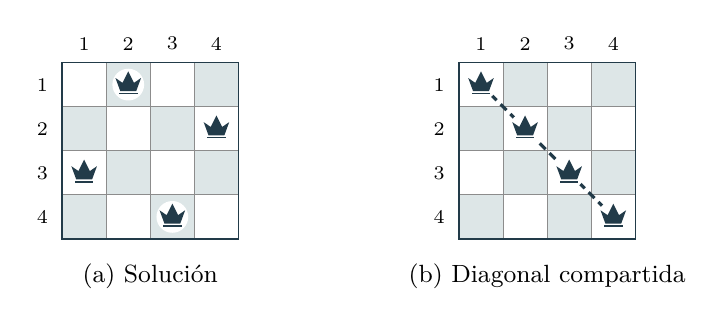
\begin{tikzpicture}[x=5.6mm,y=5.6mm]
  \begin{scope}
    \bcuadricula{4}
    \foreach \r/\c in {1/2,2/4,3/1,4/3} {\breina{4}{\r}{\c}}
    \node[font=\small,anchor=north] at (2,-.35) {(a) Solución};
  \end{scope}
  \begin{scope}[shift={(9,0)}]
    \bcuadricula{4}
    \draw[btinta,densely dashed,line width=1.1pt] (.5,3.5)--(3.5,.5);
    \foreach \r/\c in {1/1,2/2,3/3,4/4} {\breina{4}{\r}{\c}}
    \node[font=\small,anchor=north] at (2,-.35) {(b) Diagonal compartida};
  \end{scope}
\end{tikzpicture}
\caption{Dos permutaciones en el mismo tablero. Las filas se numeran de arriba abajo y las columnas
de izquierda a derecha, empezando en uno. En (a) se leen las columnas $(2,4,1,3)$: las cuatro
reinas están también en diagonales distintas de cada orientación. En (b) se leen $(1,2,3,4)$:
cada fila y cada columna sigue teniendo una reina, pero la diagonal trazada contiene las cuatro.}
\label{fig:permutaciones}
\end{figure}


¿Cuánto reducen las diagonales esas $n!$ posibilidades cuando crece el tablero?
Simkin~\cite[Teorema~1.1]{Simkin} determinó el orden principal mediante un principio variacional:
existe una constante $\alpha$ tal que
\[
 Q(n)=\bigl((1+o(1))\,n\,e^{-\alpha}\bigr)^n .
\]
Nobel, Agrawal y Boyd~\cite{NAB} acotaron $\alpha$ en $[1{,}944000752,\,1{,}944001082]$.
Al tomar logaritmos y aplicar la fórmula de Stirling, el resultado de Simkin da
\[
 \log Q(n)-\log n!=n(1-\alpha)+o(n).
\]
El resto $o(n)$ no está determinado. La pregunta que motiva este artículo es la del término
siguiente: si, tras restar el término lineal, la diferencia converge, y hacia qué constante.

Construimos una cantidad determinista $Q_{\rm pred}(n)$, que llamamos predictor, cuyo término
constante sí podemos calcular. La construcción asigna un peso a cada casilla, de manera que cada fila
y cada columna sumen uno y ninguna diagonal reciba más de uno. Entre los pesos admisibles del modelo
se eligen los que maximizan la entropía de Bethe (Sección~\ref{sec:predictor}). Esa entropía aporta
el primer término del predictor. Los otros tres términos de la Definición~\ref{def:Qpred} son un
término local, que depende de los pesos por casilla; un pseudodeterminante, en el que interviene además cómo
se cortan las líneas; y una normalización. La definición exige que el maximizador sea interior, lo
que ocurre para todo $n$ suficientemente grande (Sección~\ref{sec:P02}).

Al pasar del tablero al cuadrado unidad aparece el perfil de masa uno $\nu_1$ de~\cite{Perfil}.
Escribimos $s_1$ para el valor óptimo en masa uno, que alcanza ese perfil, y $\Phi=s_1+1$. Bajo
la identificación con el problema de Simkin que se discute en la Sección~\ref{sec:preliminares}, y
que no usamos en ninguna prueba, $\Phi=1-\alpha$. La integral $I_2=\int\nu_1^2$ se toma sobre
el cuadrado unidad. Como $\nu_1$ tiene masa total uno, $I_2\ge1$, con igualdad sólo para la densidad
constante: $I_2$ mide cuánto se aparta el perfil de ella.

\begin{teorema}[Término constante del predictor]\label{thm:intro-constante}
Cuando $n\to\infty$,
\[
\begin{aligned}
 \log Q_{\rm pred}(n)-\log n!-n\Phi &\longrightarrow C_{\rm pred},\\
 C_{\rm pred} &=\tfrac12\log2-\tfrac12-\tfrac32I_2-\tfrac12\log{\det}_2(I+J),
\end{aligned}
\]
donde $J$ es el operador de Hilbert--Schmidt construido a partir de $\nu_1$ en la
Sección~\ref{sec:D03} e $I+J$ es definido positivo.
\end{teorema}

La prueba sigue la definición término a término. Primero se aproxima el maximizador discreto por
el perfil continuo con error $O(1/n)$ (Sección~\ref{sec:perfil}). Después se identifican por
separado las contribuciones de la entropía y del pseudodeterminante, y se suman al término local
(Sección~\ref{sec:constante}). El teorema se demuestra en la Sección~\ref{sec:D05}
(Teorema~\ref{thm:constante}).

El segundo resultado responde a una pregunta que ya se puede formular en un tablero pequeño.
Una colocación parcial deja un tablero residual $B$. Elegimos una fila vacía $r$ y llamamos
$B+c$ al residual que queda tras ocupar en ella una casilla legal $c$. Si $Q(B)$ cuenta las
completaciones de $B$, entonces
\[
 Q(B)=\sum_{c\in r} Q(B+c).
\]
En efecto, cada completación usa exactamente una de esas casillas. Una elección legal que luego
no pueda completarse aporta cero a la suma. La Figura~\ref{fig:residual} muestra esta partición
en un tablero de $5\times5$ con una reina en la fila~1 y la columna~2: en la segunda fila quedan dos
casillas legales, las de las columnas 4 y~5, y cada una da un sumando.

\begin{figure}[htbp]
\centering
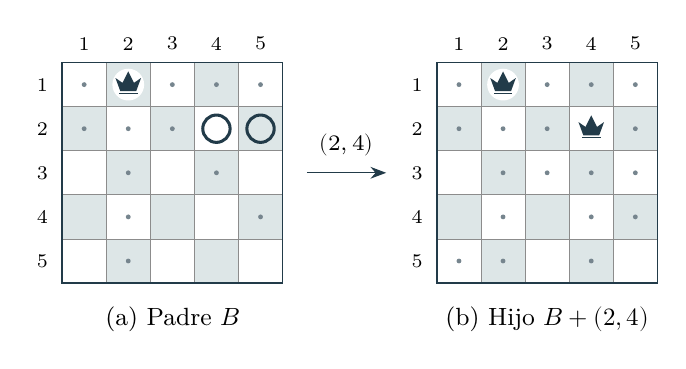
\begin{tikzpicture}[x=5.6mm,y=5.6mm]
 \begin{scope}
  \bcuadricula{5}
  \foreach \r in {1,...,5} {\foreach \c in {1,...,5} {
    \pgfmathtruncatemacro{\ataque}{(\r==1)||(\c==2)||(abs(\r-1)==abs(\c-2))}
    \ifnum\ataque=1\relax\bmarca{5}{\r}{\c}\fi
  }}
  \breina{5}{1}{2}
  \foreach \c in {4,5}{\draw[btinta,line width=1.1pt] (\c-.5,3.5) circle[radius=.31];}
  \node[anchor=north,font=\small] at (2.5,-.32) {(a) Padre $B$};
 \end{scope}
 \draw[-{Stealth[length=2mm]},btinta] (5.55,2.5)--(7.35,2.5);
 \node[font=\footnotesize,above] at (6.45,2.65) {$(2,4)$};
 \begin{scope}[shift={(8.5,0)}]
  \bcuadricula{5}
  \foreach \r in {1,...,5}{\foreach \c in {1,...,5}{
    \pgfmathtruncatemacro{\ataque}{(\r==1)||(\c==2)||(abs(\r-1)==abs(\c-2))||(\r==2)||(\c==4)||%
(abs(\r-2)==abs(\c-4))}
    \ifnum\ataque=1\relax\bmarca{5}{\r}{\c}\fi
  }}
  \breina{5}{1}{2}\breina{5}{2}{4}
  \node[anchor=north,font=\small] at (2.5,-.32) {(b) Hijo $B+(2,4)$};
 \end{scope}
\end{tikzpicture}
\caption{La partición exacta del conteo en un tablero pequeño. En la segunda fila del tablero
izquierdo hay dos opciones legales, marcadas con aros. La flecha sigue una de ellas; la otra,
$(2,5)$, da el segundo sumando del conteo. Los puntos señalan casillas ocupadas o atacadas y las
coronas identifican las reinas colocadas. Las casillas disponibles conservan sus coordenadas.}
\label{fig:residual}
\end{figure}


El predictor asigna a $B$ el valor $e^{L(B)}$ (Sección~\ref{sec:B3T01}).
Dividimos la suma de las predicciones de los hijos por la predicción del padre:
\[
 \rho(B)=\frac{\sum_{c\in r}e^{L(B+c)}}{e^{L(B)}}
        =\sum_{c\in r}e^{L(B+c)-L(B)} .
\]
Si el predictor cumpliera exactamente la misma identidad que el conteo, este cociente valdría uno.
El siguiente teorema acota el defecto en escala logarítmica y especifica para qué residuales vale
esa cota.

Su enunciado usa nociones que se precisan en las Secciones~\ref{sec:insercion} y~\ref{sec:B5T01}.
Un residual con $k$ filas vacías tiene también $k$ columnas vacías y le faltan $k$ reinas; en
\cite{Completabilidad} ese número se denota $h$.
El \emph{punto de Bethe} de $B$ es el vector de pesos $p=(p_e)$, con un peso por casilla disponible
$e$, en el que se evalúa $L(B)$: un punto estacionario de la entropía de Bethe del residual bajo las
restricciones de fila y de columna. La \emph{masa} de una diagonal, de cualquiera de las dos
familias, es la suma de los pesos de sus casillas disponibles; su \emph{vacancia} es uno menos la
masa. El \emph{laplaciano de filas y columnas} es el del grafo cuyos vértices son las filas y las
columnas vacías y en el que cada casilla disponible $e$ es una arista de peso $p_e$ entre su fila y
su columna; su \emph{brecha} es su segundo autovalor más pequeño, contado con multiplicidad.

\begin{teorema}[Consistencia de segundo orden]\label{thm:intro-consistencia}
Sean $C,\eta,\gamma>0$ y sea $B$ un residual con $k$ filas vacías cuyo punto de Bethe $p$ es
estacionario e interior, con masas de fila y columna iguales a uno, $p_e\le C/k$, vacancias diagonales
al menos $\eta$ y brecha al menos $\gamma$ del laplaciano de filas y columnas ponderado por $p$.
\begin{enumerate}[(a)]
\item Para cada $\delta_0>0$ existen $k_0$ y $C_*$, que dependen sólo de $\delta_0,C,\eta,\gamma$, tales
que, si $k\ge\max(k_0,\delta_0n)$, entonces $|\log\rho(B)|\le C_*/k^2$ para toda fila vacía $r$
(Teorema~\ref{thm:macro} y Corolario~\ref{cor:rho}).
\item Existen $\varepsilon_0$, $k_0$ y $C_*$, que no dependen de $n/k$, tales que la misma conclusión
vale para $k\ge k_0$ sin la condición $k\ge\delta_0n$ si la masa de cada diagonal es a lo sumo
$\varepsilon_0$ (Teorema~\ref{thm:meso}).
\end{enumerate}
\end{teorema}

Ambas partes incluyen todos los hijos legales de la fila elegida. Para cada hijo se obtiene un
único punto estacionario en la rama pequeña, es decir, con todos sus pesos menores que $1/4$. La
primera parte pide que quede una fracción fija de las filas originales. La segunda prescinde de esa
condición cuando la masa de cada diagonal es pequeña. En los dos casos las hipótesis recaen sobre el
residual. El teorema es determinista: no afirma que los residuales que aparecen al colocar reinas al azar cumplan esas hipótesis.

Para trasladar el primer teorema al conteo exacto falta controlar una diferencia:
\[
 R_Q(n)=\log Q(n)-\log Q_{\rm pred}(n).
\]
Si $R_Q(n)\to0$, se obtiene
\[
 \log Q(n)=\log n!+n\Phi+C_{\rm pred}+o(1).
\]
No probamos que $R_Q(n)\to0$. La Sección~\ref{sec:discusion} explica qué estimaciones adicionales
sobre las trayectorias y los residuales con pocas filas vacías exigiría ese paso.

Numéricamente, $C_{\rm pred}\approx0{,}9401$: en todo el intervalo de $\alpha$ citado, los ajustes del predictor desde $n=40$ o $60$ dan entre $0{,}9400$ y $0{,}9402$, y una evaluación directa de la fórmula da $0{,}94014$ (Sección~\ref{sec:numerico}); ninguna de estas cifras está certificada.
Con la referencia $\Phi_0$ de esa sección, los conteos exactos para $16\le n\le27$ dan $\log Q(n)-\log n!-n\Phi_0$ entre $0{,}913$ y $0{,}941$.

\subsection*{Relación con trabajos previos}

Luria y Simkin~\cite{LS} obtuvieron una cota inferior para el conteo de reinas mediante un
proceso voraz y absorción. Bowtell y Keevash~\cite{BK} estudiaron el problema toroidal y sus
consecuencias para el tablero ordinario. Aquí la construcción del predictor parte de otro
objeto, el máximo de una entropía sobre pesos de casilla.

La aproximación de Bethe y sus correcciones por lazos se han estudiado para el permanente de matrices
no negativas~\cite{Vontobel,WC} y, en general, para modelos discretos sobre grafos~\cite{CC,WF,YFW}.
La fórmula de Ihara--Bass~\cite{Bass}, en la forma de Watanabe y Fukumizu~\cite{WF}, relaciona la
corrección de un lazo con un determinante de tamaño igual al número de líneas, y es el origen
heurístico del pseudodeterminante de~\eqref{eq:Qpred}.
Para las semirreinas toroidales, Eberhard, Manners y Mrazović~\cite{EMM19} obtuvieron una asintótica
que incluye el factor constante, y después trataron las transversales de cuadrados latinos
cuasialeatorios~\cite{EMM}; en esos modelos no intervienen las dos familias de diagonales del tablero
ordinario. Liu, Liao y Wang~\cite{LLW} estudiaron el problema de las reinas como un gas reticular, con
simulaciones de Monte Carlo y redes tensoriales.
Este artículo usa los resultados de~\cite{Perfil} sobre el perfil de masa uno. En~\cite{Completabilidad}
se estudian, mediante una comparación de entropía relativa con un proceso de referencia y una doble
cuenta de reparaciones, las colocaciones legales elegidas uniformemente a las que falta un número fijo
de reinas: la fracción media de cruces vacíos (las intersecciones de las filas y las columnas vacías)
que admiten una reina tiende al inverso de la constante de normalización de ese perfil. Ese resultado
no determina el término constante del conteo exacto.

\subsection*{Organización}

Las Secciones~\ref{sec:preliminares} y~\ref{sec:predictor} pasan de las cuatro líneas de una
casilla a la fórmula del predictor. A partir de ahí, las dos preguntas del artículo se tratan por
separado. Para obtener la constante, la Sección~\ref{sec:perfil} compara el tablero finito con el
perfil continuo y la Sección~\ref{sec:constante} calcula los términos que sobreviven en el límite.
Para entender la consistencia, la Sección~\ref{sec:insercion} estudia una inserción y las
Secciones~\ref{sec:macro} y~\ref{sec:meso} controlan su efecto en los dos regímenes del teorema.

La Sección~\ref{sec:numerico} contrasta dos evaluaciones de la constante del predictor con los
valores del conteo exacto para $16\le n\le27$. La Sección~\ref{sec:discusion} distingue esos resultados
de la cuestión abierta sobre $Q(n)$. El Apéndice~\ref{sec:torres} ofrece un caso explícito
en el que se conservan sólo las restricciones de filas y columnas.

\section{Preliminares}\label{sec:preliminares}

\paragraph{Tablero y líneas.}
Las casillas del tablero son los pares $(i,j)$ con $1\le i,j\le n$; $i$ es la fila y $j$ la columna.
Hay cuatro familias de líneas: las filas $R_i$, las columnas $C_j$, las diagonales
$D_k=\{i-j=k\}$, $-n<k<n$, y las antidiagonales $A_l=\{i+j-1=l\}$, $0<l<2n$. Son $n$, $n$,
$2n-1$ y $2n-1$ líneas, $6n-2$ en total. Cada casilla está en exactamente cuatro líneas, una de cada
familia, y dos líneas de familias distintas se cortan en a lo sumo una casilla.
Numeramos filas y columnas desde uno, y no desde cero como en~\cite{Perfil}
y~\cite{Completabilidad}: la casilla $(i,j)$ de este artículo es allí la $(i-1,j-1)$, la diagonal
$D_k$ es la de diferencia $k$ y la antidiagonal $A_l$ es la de suma $l-1$.
En la Figura~\ref{fig:incidencia} se pueden leer las cuatro etiquetas de una sola casilla.
\begin{figure}[htbp]
\centering
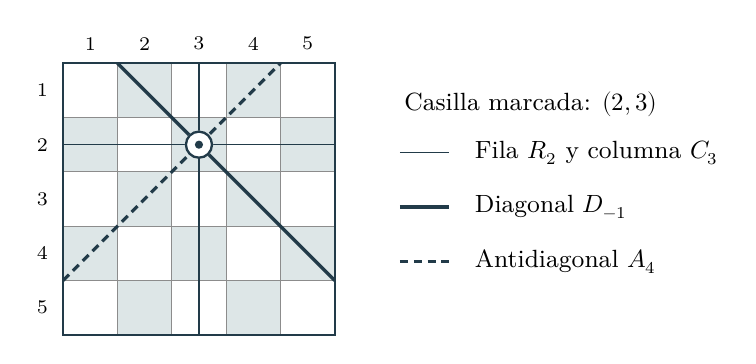
\begin{tikzpicture}[x=6.9mm,y=6.9mm]
 \bcuadricula{5}
 \draw[btinta,thin] (0,3.5)--(5,3.5);
 \draw[btinta,thin] (2.5,0)--(2.5,5);
 \draw[btinta,line width=1.2pt] (1,5)--(5,1);
 \draw[btinta,densely dashed,line width=1.1pt] (0,1)--(4,5);
 \fill[bpapel] (2.5,3.5) circle[radius=.26];
 \draw[btinta,line width=.85pt] (2.5,3.5) circle[radius=.24];
 \fill[btinta] (2.5,3.5) circle[radius=.075];
 \node[anchor=west,font=\small] at (6.1,4.25) {Casilla marcada: $(2,3)$};
 \draw[btinta] (6.2,3.35)--(7.1,3.35);
 \node[anchor=west,font=\small] at (7.4,3.35) {Fila $R_2$ y columna $C_3$};
 \draw[btinta,line width=1.2pt] (6.2,2.35)--(7.1,2.35);
 \node[anchor=west,font=\small] at (7.4,2.35) {Diagonal $D_{-1}$};
 \draw[btinta,densely dashed,line width=1.1pt] (6.2,1.35)--(7.1,1.35);
 \node[anchor=west,font=\small] at (7.4,1.35) {Antidiagonal $A_4$};
\end{tikzpicture}
\caption{Las cuatro líneas que pasan por $(2,3)$. Los índices de la diagonal y de la antidiagonal
se calculan con las coordenadas de la casilla: $2-3=-1$ y $2+3-1=4$. En la matriz de incidencia, la
fila de esta casilla tiene un uno en la columna de cada una de las cuatro líneas señaladas.}
\label{fig:incidencia}
\end{figure}


Escribimos $A$ para la matriz de incidencia, con una fila por casilla y una columna por línea.
Para $p\in\mathbb R^{n^2}$ y una línea $L$ ponemos
\[
 m_L(p)=\sum_{c\in L}p_c,\qquad h_L(p)=1-m_L(p).
\]

La cantidad $m_L$ es la masa asignada a $L$, y $h_L$, lo que le falta para llegar a uno, es su vacancia.
Por ejemplo, si se reparte uniformemente $1/5$ en cada casilla del tablero de la figura, cada
fila suma uno y la diagonal $D_{-1}$ suma $4/5$: su vacancia es $1/5$.

\paragraph{El perfil continuo de masa uno.}
Para comparar tableros de tamaños distintos se divide cada coordenada por $n$ y se
trabaja en un cuadrado fijo. Las líneas discretas dan entonces proyecciones del perfil.
Seguimos la notación de~\cite{Perfil}. En el cuadrado $[0,1]^2$, con coordenadas $(r,c)$, las
proyecciones de las cuatro familias son $\ell_R=r$, $\ell_C=c$, $\ell_D=r-c$ y $\ell_A=r+c$, con
valores en $I_R=I_C=[0,1]$, $I_D=[-1,1]$ e $I_A=[0,2]$. Para una densidad $\nu\ge0$, $m_f$ es su
proyección sobre la familia $f$ y $u_f=1-m_f$ su vacancia. La clase admisible de masa uno,
$\mathcal A_1$, está formada por las densidades de masa uno con $m_f\le1$ en casi todo punto, y
\[
 s[\nu]=-3-\int_{[0,1]^2}\nu\log\nu-\sum_{f}\int_{I_f}u_f\log u_f
\]
es el funcional de~\cite[(1.1)]{Perfil} en masa uno. Por~\cite[Teorema~1.1]{Perfil}, $s$ alcanza su
supremo en $\mathcal A_1$ en una única densidad $\nu=\nu_1$. Definimos el valor óptimo en masa
uno, que en~\cite{Perfil} se escribe $s^*(1)$ y aquí, como en~\cite{Completabilidad}, $s_1$, y dos
cantidades asociadas:
\begin{equation}\label{eq:s1}
 s_1=s[\nu_1]=\sup_{\nu\in\mathcal A_1}s[\nu],\qquad \Phi=s_1+1,\qquad I_2=\int_{[0,1]^2}\nu_1^2 .
\end{equation}
En masa uno las vacancias de filas y columnas son nulas, de modo que sólo contribuyen las de las
diagonales. Según~\cite[Observación~2.3]{Perfil}, $s$ tiene entonces, sobre las densidades admisibles,
la misma expresión que la entropía del problema variacional de
Simkin~\cite[Definición~2.9]{Simkin}. En~\cite{Simkin}, $-\alpha$ es el máximo de esa entropía en
una clase de medidas definida por clausura (Teorema~2.24 y Lema~2.22), y la Observación~2.7 de ese
artículo precisa, para las medidas absolutamente continuas, la relación entre esa clase y la
definida por las restricciones de proyección. Con la correspondencia anterior y esa observación se
seguiría $\alpha=-s_1$, es decir, $\Phi=1-\alpha$ y $\log Q(n)=\log n!+n\Phi+o(n)$. Llamamos a esto
la identificación con el problema de Simkin. No la usamos en ninguna prueba: la definición
$\Phi=s_1+1$ y los teoremas del predictor son independientes de ella.

Por~\cite[Teoremas~1.2 y~1.3 y Proposición~5.2]{Perfil}, el perfil de masa uno se factoriza como
\begin{equation}\label{eq:factorizacion}
 \nu_1(r,c)=b_0\,r_R(r)\,r_C(c)\,u_D(r-c)\,u_A(r+c),
\end{equation}
con $b_0>0$ y funciones $r_R,r_C,u_D,u_A$ continuas, positivas y Lipschitz, $\int_0^1r_R=\int_0^1r_C=1$.
En esos resultados, estos factores son los límites del perfil reescalado en el tablero lleno y
se escriben $b_0$, $r_{R,0}$, $r_{C,0}$, $u_{D,0}$ y $u_{A,0}$; como en~\cite{Completabilidad},
omitimos el subíndice salvo en la constante $b_0$.
Las marginales de filas y columnas de $\nu_1$ valen uno, y $u_f+m_f=1$ para $f=D,A$, donde
$m_f$ es la proyección de $\nu_1$ sobre la familia $f$. Existen constantes positivas
$c_\nu\le C_\nu$, $\kappa_\nu\le1$ y $L_\nu$ tales que
\[
 c_\nu\le\nu_1\le C_\nu,\qquad \kappa_\nu\le u_D,u_A\le1,
\]
y $L_\nu$ es una constante de Lipschitz de $\nu_1$ para la distancia del máximo. Las Secciones~\ref{sec:perfil}
y~\ref{sec:constante} usan del perfil continuo sólo estas propiedades. En ellas escribimos $\nu$
por $\nu_1$.

\paragraph{Convenciones.}
Las constantes $C,c,M,\eta,\kappa,\dots$ no dependen de $n$ salvo que se indique lo contrario;
$O(\cdot)$ y $o(\cdot)$ se refieren a $n\to\infty$. En las Secciones~\ref{sec:insercion}
a~\ref{sec:meso} el parámetro es el número $k$ de filas vacías: allí $O(\cdot)$ se refiere a
$k\to\infty$, y cada sección indica de qué dependen las constantes. La letra $h$, que
en~\cite{Completabilidad} designa ese número, se usa aquí para las vacancias. En las Secciones~\ref{sec:perfil}
y~\ref{sec:constante} las ecuaciones llevan rótulos propios de cada subsección, como (P1.3) o (D2.5).
En los logaritmos de normalización $\log(4\pi n)$ y $\log(2\pi)$, en la fórmula de Stirling, en el
punto de Slater de la Sección~\ref{sec:P01} y en el Apéndice~\ref{sec:torres}, $\pi$ denota
$3{,}14159\ldots$; en el resto, $\pi=\pi^{(n)}$ es el maximizador canónico y $\pi_c$ el peso de la
casilla $c$. Algunas letras que en~\cite{Perfil} tienen un significado fijo, como $\rho$, $x$, $\lambda$,
$\ell$, $u$, $F$, $J$, $L$ o $\mathcal H$, designan en algunas secciones de este artículo otros objetos,
que se definen donde aparecen; por ejemplo, $\rho(B)$ no es una masa.

\section{El predictor canónico}\label{sec:predictor}

En el conteo exacto, cada colocación es una lista de casillas ocupadas. Para construir
el predictor se trabaja con otra variable: un peso $p_{ij}$ en cada casilla. Las sumas por
fila, columna y diagonal expresan las restricciones que el modelo conserva. Entre todos los
repartos de pesos admisibles se escoge uno solo: el que maximiza el funcional que sigue.

\paragraph{El funcional canónico.}
Sea $\mathcal D$ la unión de las dos familias diagonales, con $|\mathcal D|=4n-2$. Consideramos el
politopo y el funcional
\begin{equation}\label{eq:Kn}
 K_n=\Bigl\{p\in[0,1/4]^{n^2}:\ \sum_jp_{ij}=\sum_ip_{ij}=1,\ m_d(p)\le1\ (d\in\mathcal D)\Bigr\},
\end{equation}
\begin{equation}\label{eq:Hn}
 H_n(p)=\sum_{ij}\bigl\{-p_{ij}\log p_{ij}+3(1-p_{ij})\log(1-p_{ij})\bigr\}-\sum_{d\in\mathcal D}h_d(p)\log
h_d(p),
\end{equation}
con $0\log0=0$. Este funcional es la entropía de Bethe~\cite{YFW} del sistema de filas, columnas y
diagonales, escrita en las variables de casilla y restringida a las colocaciones fraccionarias de
masa total $n$.
El tope $p\le1/4$ es el que hace cóncavo el término de casilla.

\begin{lema}[El maximizador canónico]\label{lem:maximizador}
Para $n\ge4$, $K_n$ es un convexo compacto no vacío y $H_n$ es continua en $K_n$ y estrictamente cóncava
a lo largo de todo segmento de $K_n$. En consecuencia, $H_n$ tiene un único maximizador en $K_n$, que
denotamos por $\pi^{(n)}$ y llamamos maximizador canónico.
\end{lema}
\begin{proof}
La colocación uniforme $p\equiv1/n$ está en $K_n$ si $n\ge4$, porque cada diagonal tiene a lo sumo $n$
casillas. Escribimos $H_n(p)=\sum_cf(p_c)+\sum_{d\in\mathcal D}G(m_d(p))$, con
$f(t)=-t\log t+3(1-t)\log(1-t)$ en $[0,1/4]$ y $G(z)=-(1-z)\log(1-z)$ en $[0,1]$. Ambas son continuas en
sus intervalos cerrados, y $f''(t)=-1/t+3/(1-t)<0$ en $(0,1/4)$.

Sean $p^0\ne p^1$ en $K_n$, $p^t=(1-t)p^0+tp^1$ e $I=\{c:p^0_c\ne p^1_c\}\ne\emptyset$. Para $c\in I$ y
$t\in(0,1)$, $p^t_c$ está estrictamente entre $p^0_c$ y $p^1_c$, luego en $(0,1/4)$; así
$t\mapsto f(p^t_c)$ es de clase $C^2$ en $(0,1)$ con segunda derivada $f''(p^t_c)(p^1_c-p^0_c)^2<0$.
Las casillas fuera de $I$ dan constantes. Cada $t\mapsto G(m_d(p^t))$ es cóncava, porque $G$ es cóncava
en $[0,1]$ y $m_d$ es afín. La suma $\varphi(t)=H_n(p^t)$ es continua en $[0,1]$ y estrictamente cóncava
en $(0,1)$, luego cóncava en $[0,1]$. Si fallara la desigualdad estricta entre dos puntos
$t_0<t_1$ de $[0,1]$, $\varphi$ tocaría su cuerda en un punto interior de $[t_0,t_1]$ y sería afín en
ese intervalo, en contra de la concavidad estricta en $(t_0,t_1)$. La existencia del maximizador se sigue
de la compacidad, y la unicidad, de la concavidad estricta.
\end{proof}

\begin{definicion}\label{def:Hinf}
Decimos que se cumple $(H_\infty)$ si el maximizador canónico es interior:
$0<\pi^{(n)}_c<1/4$ para toda casilla $c$ y $h_d(\pi^{(n)})>0$ para toda diagonal $d$.
\end{definicion}

La Sección~\ref{sec:P02} prueba que $(H_\infty)$ se cumple para todo $n\ge n_0$, con
$c/n\le\pi^{(n)}_{ij}\le M/n$ y $h_d\ge\eta$ para constantes positivas $c$, $M$ y $\eta$
(véase~(P2.7)). El umbral $n_0$ que da esa prueba es muy grande (final de la Sección~\ref{sec:P02}).
Para $n=4$ la hipótesis no se cumple y para $n=5$ el cálculo numérico indica que tampoco
(Sección~\ref{sec:discusion}); para $6\le n<n_0$ no está demostrada, y en los tamaños de la
Sección~\ref{sec:numerico} se comprueba numéricamente.
En lo que sigue escribimos $\pi=\pi^{(n)}$ cuando no haya ambigüedad.

\paragraph{El pseudodeterminante y el término local.}
Sea $n\ge4$ tal que su maximizador cumpla $(H_\infty)$. Ponemos
\begin{equation}\label{eq:gS}
 g_c=\frac{\pi_c(1-\pi_c)}{1-4\pi_c},\qquad
 S_n=\operatorname{diag}(0_R,0_C,h_D,h_A)+A^T\operatorname{diag}(g)A,
\end{equation}
una matriz simétrica indexada por las $6n-2$ líneas, y $v_0=(\mathbf1_R,-\mathbf1_C,0_D,0_A)$. La
forma cuadrática de $S_n$ es una suma de cuadrados cuyos pesos, $h_d$ y $g_c$, son positivos por
$(H_\infty)$. Si se anula en un vector
$x=(x_R,x_C,x_D,x_A)$, entonces $x_D=0$, $x_A=0$ y $x_{R,i}+x_{C,j}=0$ para cada casilla $(i,j)$. Por
tanto su núcleo es la recta generada por $v_0$ y $S_n$ es definida positiva en $v_0^\perp$. Para
$n\ge n_0$ la Sección~\ref{sec:P03}
da además una brecha uniforme. Llamamos \emph{gauge} a la dirección $v_0$, análoga discreta del modo neutro
$(1,-1,0,0)$
de~\cite[Sección~7.2]{Perfil}, y a su análoga en los tableros
residuales: como $Av_0=0$, sumar un múltiplo de $v_0$ a un vector indexado por las líneas no cambia sus
sumas por casilla. Fijar el gauge es elegir un representante, por ejemplo en $v_0^\perp$. El
pseudodeterminante
$\operatorname{pdet}S_n$ es el producto de sus autovalores no nulos. El término local es
\[
 L_n=-\frac12\sum_{ij}\bigl[\log(1-4\pi_{ij})-4\log(1-\pi_{ij})\bigr],
\]
como en~(LC1).

\begin{definicion}[Predictor canónico]\label{def:Qpred}
Para $n\ge4$ que cumpla $(H_\infty)$,
\begin{equation}\label{eq:Qpred}
 \log Q_{\rm pred}(n)=H_n(\pi^{(n)})+L_n-\tfrac12\log\operatorname{pdet}S_n+\tfrac12\log(4\pi n).
\end{equation}
\end{definicion}

\begin{observacion}[Origen de la definición]
De los cuatro términos de la definición, el primero es la entropía de Bethe en su máximo. Los otros
tres corresponden, heurísticamente, a dos ingredientes más: la corrección de un lazo de la
aproximación de Bethe, escrita como determinante de la matriz hessiana mediante la fórmula de
Ihara--Bass en la forma de Watanabe y Fukumizu~\cite{Bass,WF}, y la normalización gaussiana del modo
cero que impone la igualdad entre el número de filas vacías y el de columnas vacías. Sobre estas
aproximaciones para permanentes y sistemas en grafos pueden verse~\cite{CC,ChertkovYedidia,Vontobel},
y sobre las correcciones de lazos a la aproximación de Bethe,~\cite{MontanariRizzo}. En el modelo
de torres, una fórmula con los mismos tres ingredientes aproxima el logaritmo del conteo con error
$O(1/k)$ hasta el tablero lleno (Apéndice~\ref{sec:torres}). En este artículo \eqref{eq:Qpred} es
sólo una definición: ninguna prueba usa esa interpretación ni el apéndice.
\end{observacion}

Para los tableros residuales que aparecen al colocar reinas una a una, el predictor $L(B)$ se define en
la Sección~\ref{sec:B3T01}, con el mismo funcional, el determinante canónico del residual y la
normalización $\tfrac12\log(2\pi)$ por componente. En el tablero completo, $L(B)$ coincide con
$\log Q_{\rm pred}(n)$ (Lema~\ref{lem:puente}).

\section{El perfil canónico discreto}\label{sec:perfil}

El paso del tablero al cuadrado unidad exige comparar magnitudes de la misma escala.
Como las $n$ casillas de cada fila suman uno, su peso medio es $1/n$. Por ello comparamos
$n\pi_{ij}$, y no el peso sin reescalar, con el valor de $\nu_1$ en el centro de la casilla.

Primero hay que asegurar que el maximizador se mantiene alejado de los extremos en el sentido
preciso de la Sección~\ref{sec:P02}: sus pesos están entre $c/n$ y $M/n$ y las vacancias
diagonales tienen una cota inferior positiva. La Sección~\ref{sec:P01} prepara esas cotas
mediante un punto de Slater, es decir, un punto factible que cumple con desigualdad estricta las
restricciones diagonales y de casilla.
Con ellas se controla el espectro de $S_n$ en la Sección~\ref{sec:P03} y se desarrolla el
término local en la Sección~\ref{sec:P04}. Finalmente, las Secciones~\ref{sec:P05}
y~\ref{sec:P06} establecen la comparación anunciada con error uniforme $O(1/n)$.

\subsection{Punto de Slater y cota de los multiplicadores del tope}\label{sec:P01}
Del Lema~\ref{lem:maximizador} sólo se usa la existencia y unicidad del maximizador canónico;
no se presupone su interioridad ni se afirma que coincida con las probabilidades de ocupación de las
casillas en una solución elegida uniformemente al azar.
Recordamos que $\mathcal D$ es la unión de las dos familias diagonales del tablero,
con $|\mathcal D|=4n-2$, y que
\[
 m_d(p)=\sum_{c\in d}p_c,\qquad h_d(p)=1-m_d(p).
\]
El politopo $K_n$ y el funcional $H_n$ son los de~\eqref{eq:Kn} y~\eqref{eq:Hn}, con la convención
$0\log0=0$. Denotamos por $p=\pi^{(n)}$ el único maximizador de $H_n$ en $K_n$.

\paragraph{Un punto de Slater para $n\ge32$.}
Sean $r_i=(i-1/2)/n$ y
\[
 q_{ij}=\frac1n\left[1-\frac15\cos(2\pi r_i)\cos(2\pi r_j)\right].
\]
La suma de los cosenos de los $n$ puntos medios es cero para $n\ge2$;
por tanto las sumas de filas y columnas de $q$ son exactamente uno y
$4/(5n)\le q_{ij}\le6/(5n)$.
La densidad estrictamente admisible $\nu^\sharp(r,c)=1-\frac15\cos(2\pi r)\cos(2\pi c)$
de~\cite[Observación~2.4]{Perfil} tiene, para $0\le d\le1$, la marginal
\[
 m_D[\nu^\sharp](d)=1-d-\frac15\left[
       \frac{1-d}{2}\cos(2\pi d)-\frac{\sin(2\pi d)}{4\pi}\right].
\]
Su derivada es a lo sumo $-1+(1+\pi)/5<0$, luego $m_D[\nu^\sharp]\le9/10$.
Las simetrías dan la misma cota en las dos familias completas.
Cada suma diagonal de $q$ es una cuadratura de puntos medios de
$\nu^\sharp$ en la fibra correspondiente, con extremos múltiplos de $1/n$.
La longitud paramétrica de la fibra es a lo sumo uno y su constante
de Lipschitz es a lo sumo $4\pi/5$. El error de cuadratura es, pues,
a lo sumo $(4\pi/5)/(2n)\le1/20$ para $n\ge32$, usando $\pi<4$.
En consecuencia, con $M_0=6/5$ y $\kappa=1/20$,
\[
 q_{ij}\le M_0/n<1/8,\qquad h_d(q)\ge\kappa.       \tag{P1.1}
\]
Se obtiene así un punto de Slater en el espacio afín de las sumas de filas y columnas.

\paragraph{Positividad en presencia del tope.}
Tomamos $p(t)=(1-t)p+tq$. Si $p_c=0$, su entropía espacial aporta
$-q_c t\log t+O(t)$ a $H_n(p(t))-H_n(p)$. Si $h_d(p)=0$, su
entropía diagonal aporta $-h_d(q)t\log t+O(t)$. Las demás entropías
aportan $O(t)$; también lo hace $3(1-p)\log(1-p)$, cuya derivada
está acotada en $[0,1/4]$. Si se da alguna de esas igualdades, la
diferencia es $-At\log t+O(t)>0$ para $t>0$ pequeño, con $A>0$,
lo que contradice la maximalidad. Por ello
\[
 p_{ij}>0,\qquad h_d(p)>0.                         \tag{P1.2}
\]

\paragraph{Condiciones de optimalidad con multiplicadores del tope.}
Por (P1.2), el funcional es diferenciable cerca de $p$ y las únicas desigualdades
potencialmente activas son $p_{ij}\le1/4$.
La condición de Slater proporciona multiplicadores finitos $\alpha_i,\beta_j$ y
$\mu_{ij}\ge0$. Una de las igualdades de filas y columnas es redundante y se suprime
al aplicar las condiciones de Karush--Kuhn--Tucker (KKT)~\cite[cap.~5]{BV}. Si $D(i,j),A(i,j)$ son las
dos diagonales de la casilla, resulta
\[
 -\log p_{ij}-3\log(1-p_{ij})+\log h_{D(i,j)}+\log h_{A(i,j)}-2
 =\alpha_i+\beta_j+\mu_{ij},\quad
 \mu_{ij}(1/4-p_{ij})=0.                          \tag{P1.3}
\]
Sean $x_{ij}=np_{ij}$, $\ell_d=-\log h_d(p)\ge0$ y
$d_0=3\log(4/3)$. Multiplicando (P1.3) por $q_{ij}-p_{ij}$ y
sumando se cancelan las igualdades y la constante $-2$. Se obtiene
\[
 0=E+F+Q+U,                                      \tag{P1.4}
\]
\[
 E=\sum_{ij}(p_{ij}-q_{ij})\log x_{ij},\qquad
 F=3\sum_{ij}(p_{ij}-q_{ij})\log(1-p_{ij}),
\]
\[
 Q=\sum_{d\in\mathcal D}(h_d(q)-h_d(p))\ell_d,\qquad
 U=\sum_{ij}\mu_{ij}(1/4-q_{ij}).
\]
En particular $U$ lleva signo positivo: la derivada hacia $q-p$
es $-U$, por complementariedad.

\paragraph{Cota global que incluye los multiplicadores del tope.}
La convexidad da $\sum p_{ij}\log(np_{ij})\ge0$. Además
\[
 \sum q_{ij}\log x_{ij}\le\frac{M_0}{n}\sum\log^+x_{ij}
 \le\frac{M_0}{n}\sum x_{ij}=M_0n,
\]
de modo que $E\ge-M_0n$. Como $\log(1-p)\le0$,
\[
 F\ge3\sum p_{ij}\log(1-p_{ij})\ge-d_0n.
\]
La desigualdad $h(-\log h)\le1/e$ y (P1.1) dan
\[
 Q\ge\kappa\sum_d\ell_d-4n/e,\qquad
 U\ge\frac18\sum_{ij}\mu_{ij}.
\]
Por (P1.4), si $C_0=M_0+d_0+4/e$,
\[
 \kappa\sum_d\ell_d+\frac18\sum_{ij}\mu_{ij}\le C_0n.
\]
Como $\kappa\le1/8$, con $T=C_0/\kappa$ queda
\[
 \frac1n\left(\sum_d\ell_d+\sum_{ij}\mu_{ij}\right)\le T.    \tag{P1.5}
\]
Esta estimación no presupone que ningún multiplicador $\mu$ sea cero.

\subsection{Cotas uniformes de los pesos y de las vacancias; interioridad}\label{sec:P02}
Se mantienen las notaciones de la Sección~\ref{sec:P01}, en particular
$n\ge32$, $\kappa=1/20$, $M_0=6/5$, $d_0=3\log(4/3)$ y
$T=(M_0+d_0+4/e)/\kappa$.

\paragraph{Factorización con el multiplicador presente.}
La ecuación (P1.3) admite la factorización
\[
 x_{ij}=B R_i C_j K_{ij},\qquad
 K_{ij}=h_{D(i,j)}h_{A(i,j)}e^{-\mu_{ij}}(1-p_{ij})^{-3},
                                                               \tag{P2.1}
\]
con factores positivos y normalizaciones geométricas
\[
 \frac1n\sum_i\log R_i=\frac1n\sum_j\log C_j=0.
\]
Se obtienen, por ejemplo, dividiendo $e^{-\alpha_i}$ y
$e^{-\beta_j}$ por sus medias geométricas y absorbiendo en $B$
esos dos factores escalares junto con $ne^{-2}$.
Cada fila encuentra como máximo una vez cada diagonal de cada
familia. Por tanto, (P1.5) y la desigualdad $(1-p)^{-3}\ge1$ dan
\[
 \frac1n\sum_j\log K_{ij}\ge-T.
\]
La misma propiedad vale para cada columna:
\[
 \frac1n\sum_i\log K_{ij}\ge-T.                  \tag{P2.2}
\]
Aquí se usa la suma global de $\mu$: la suma de sus valores en una
fila o columna es menor o igual a esa suma global.

\paragraph{Control de los factores sin suponer vacancia puntual.}
La desigualdad de Jensen, las normalizaciones geométricas y las sumas de filas dan
\[
 1=B R_i\frac1n\sum_j C_jK_{ij}\ge B R_i e^{-T}.
\]
Aplicando lo mismo a las columnas,
\[
 R_i,C_j\le e^T/B.                               \tag{P2.3}
\]
Por otro lado $\log K_{ij}\le d_0$, pues $h_d\le1$,
$\mu_{ij}\ge0$ y $p_{ij}\le1/4$.
Multiplicamos el logaritmo de (P2.1) por $p_{ij}$ y sumamos.
Las contribuciones de $\log R_i$ y $\log C_j$ desaparecen: las
sumas de filas y columnas son uno y sus sumas de logaritmos son
cero. Por la convexidad ya usada en la Sección~\ref{sec:P01},
\[
 n\log B=\sum_{ij}p_{ij}\log(np_{ij})
               -\sum_{ij}p_{ij}\log K_{ij}\ge-d_0n.
\]
Así $B\ge e^{-d_0}$. De (P2.3) se deduce la cota
\[
 B R_i C_j(1-p_{ij})^{-3}
 \le e^{2T+d_0}/B\le e^{2T+2d_0}=:M.             \tag{P2.4}
\]
En (P2.1) todos los factores $h_d,e^{-\mu_{ij}}$ son a lo sumo
uno. Por ello, todavía sin retirar los topes,
\[
             0<p_{ij}\le M/n.                    \tag{P2.5}
\]

\paragraph{Vacancias uniformes.}
Fijada una diagonal $d$ de la primera familia, (P2.1) y (P2.4) dan
\[
 m_d(p)=\frac{h_d}{n}\sum_{(i,j)\in d}
 B R_i C_j h_{A(i,j)}e^{-\mu_{ij}}(1-p_{ij})^{-3}
 \le M h_d\frac{|d|}{n}\le M h_d.
\]
El mismo argumento se aplica a la segunda familia.
Como $m_d=1-h_d$, resulta para todas las diagonales
\[
                 h_d\ge\eta:=\frac1{1+M}.        \tag{P2.6}
\]
También esta conclusión es anterior a la retirada del tope.

\paragraph{Retirada del tope y cota inferior.}
Para
\[
 n\ge n_0:=\max\{32,\lfloor4M\rfloor+1\},
\]
(P2.5) implica $p_{ij}<1/4$. La complementariedad da entonces
$\mu_{ij}=0$ en todas las casillas.
Así se obtienen la hipótesis $(H_\infty)$ de la Definición~\ref{def:Hinf} y
las cotas uniformes. De hecho, las cotas (P2.5) y
(P2.6) valen ya para todo $n\ge32$.
Para $n\ge n_0$ se tiene además una cota inferior de orden $1/n$.
De $K_{ij}\le e^{d_0}$ y (P2.3), la ecuación de fila implica
\[
 R_i=\left(B\frac1n\sum_jC_jK_{ij}\right)^{-1}
       \ge e^{-(T+d_0)};
\]
análogamente $C_j\ge e^{-(T+d_0)}$.
Una vez que $\mu=0$, (P2.6) da $K_{ij}\ge\eta^2$. Junto con
$B\ge e^{-d_0}$, esto prueba
\[
 \frac{c}{n}\le p_{ij}\le\frac Mn,\qquad
 c:=\eta^2e^{-2T-3d_0}>0,
 \qquad h_d\ge\eta.                              \tag{P2.7}
\]

\subsection{Brecha uniforme del operador canónico reducido}\label{sec:P03}
Se usan exclusivamente las cotas deterministas de la Sección~\ref{sec:P02}.
Sea $n$ suficientemente grande para que
\[
 c/n\le\pi_{ij}\le M/n\le1/8,\qquad h_D,h_A\ge\eta>0.
\]
Los símbolos $c,M,\eta$ son constantes, no índices de casilla.
La matriz de incidencia $A$ tiene una fila por casilla y una columna por línea.
Ponemos
\[
 g_{ij}=\frac{\pi_{ij}(1-\pi_{ij})}{1-4\pi_{ij}},\quad
 S=\operatorname{diag}(0_R,0_C,h_D,h_A)+A^T\operatorname{diag}(g)A.
                                                        \tag{G1}
\]
Entonces $c/n\le g_{ij}\le2M/n$.
Se usan normas euclídeas ordinarias en las $6n-2$ líneas.

\begin{proposicion}
El núcleo de $S$ es exactamente
$\operatorname{span}\{v_0\}$, con
$v_0=(\mathbf1_R,-\mathbf1_C,0_D,0_A)$.
En $v_0^\perp$ se tiene
\[
 \gamma\|v\|^2\le v^TSv\le(1+8M)\|v\|^2,
 \qquad \gamma=\min\{c/2,\eta/5\}>0.               \tag{G2}
\]
Las constantes son independientes de $n$.
\end{proposicion}
\begin{proof}
Escribimos $v=(r_i,t_j,d_k,a_l)$ y
$s_{ij}=r_i+t_j+d_{i-j}+a_{i+j-1}$.
La condición $v\perp v_0$ equivale a $\sum_i r_i=\sum_jt_j$.
Por tanto
\[
 \frac1n\sum_{ij}(r_i+t_j)^2
 =\sum_i r_i^2+\sum_jt_j^2+
       \frac2n\left(\sum_i r_i\right)^2
 \ge\|r\|^2+\|t\|^2.
\]
La desigualdad $(s-d-a)^2\le2s^2+4(d^2+a^2)$
y el hecho de que cada diagonal tiene a lo sumo $n$ casillas
dan
\[
 \|v\|^2\le\frac2n\sum_{ij}s_{ij}^2
                        +5(\|d\|^2+\|a\|^2).     \tag{G3}
\]
Por (G1),
\[
 v^TSv\ge\frac cn\sum s_{ij}^2+
                          \eta(\|d\|^2+\|a\|^2),
\]
lo que prueba la cota inferior. Además
$s_{ij}^2\le4(r_i^2+t_j^2+d_{i-j}^2+a_{i+j-1}^2)$.
Cada línea tiene a lo sumo $n$ casillas, así que
$\sum s_{ij}^2\le4n\|v\|^2$. Como $h_D,h_A\le1$,
se obtiene la cota superior.
Finalmente $Sv_0=0$. Si $v^TSv=0$, la positividad de
$g,h_D,h_A$ obliga a $d=a=0$ y $r_i+t_j=0$ para todo $i,j$.
Luego $r$ es constante y $t$ su opuesto: no hay otros ceros.
\end{proof}

\paragraph{Consecuencia.}
La inversa de $S$ sobre $v_0^\perp$ tiene norma espectral
a lo sumo $\gamma^{-1}$, con $\gamma$ independiente de $n$.

\subsection{El término local de la fórmula canónica}\label{sec:P04}
Se toma $n$ suficientemente grande, en particular $n\ge8M$.
Se distingue una consecuencia de la Sección~\ref{sec:P02} de otra que requiere
la comparación con el perfil continuo (Secciones~\ref{sec:P05} y~\ref{sec:P06}).
El término local es
\[
 L_n=-\frac12\sum_{ij}
       [\log(1-4\pi_{ij})-4\log(1-\pi_{ij})].       \tag{LC1}
\]
Para $0\le t\le1/8$, las series escalares convergentes dan
\[
 -\tfrac12[\log(1-4t)-4\log(1-t)]
   =\frac12\sum_{m\ge2}\frac{4^m-4}{m}t^m.
\]
El término cuadrático es $3t^2$ y los restantes son positivos.
Su suma está acotada por
\[
 \frac12\sum_{m\ge3}(4t)^m
       =\frac{32t^3}{1-4t}\le64t^3.
\]
Con $\pi\le M/n$ y $\sum\pi=n$ resulta
\[
 0\le L_n-3\sum_{ij}\pi_{ij}^2
       \le64\sum\pi_{ij}^3\le\frac{64M^2}{n}.      \tag{LC2}
\]
La estimación (LC2) es una expansión local de escala $\pi=O(1/n)$.

\paragraph{Paso del término local al perfil continuo.}
Si $\nu_1$ es el perfil continuo acotado y Lipschitz y
\[
 \max_{ij}|n\pi_{ij}-\nu_1((i-1/2)/n,(j-1/2)/n)|=O(1/n),
                                                        \tag{LC3}
\]
entonces
\[
 \sum_{ij}\pi_{ij}^2
       =\int_{[0,1]^2}\nu_1(r,c)^2\,dr\,dc+O(1/n).
\]
En efecto, el error entre los cuadrados de los perfiles
es $O(1/n)$ uniformemente, y la cuadratura bidimensional
de una función Lipschitz tiene error $O(1/n)$.
Por (LC2),
\[
 L_n=3\int_{[0,1]^2}\nu_1^2+O(1/n).               \tag{LC4}
\]
Éste es sólo uno de los sumandos de $\log Q_{\rm pred}$; las contribuciones de la entropía y
del pseudodeterminante se estudian en la Sección~\ref{sec:constante}.

Las Secciones~\ref{sec:P05} y~\ref{sec:P06} prueban (LC3) para el maximizador canónico;
por tanto (LC4) se aplica a él.

\subsection{Comparación con el perfil continuo: sistema y residuo}\label{sec:P05}
\paragraph{Datos de partida.}
Las Secciones~\ref{sec:P01} y~\ref{sec:P02} proporcionan, para el maximizador canónico $\pi$ y
$n\ge n_0$, el umbral de la Sección~\ref{sec:P02},
\[
 c\le\rho^*_{ij}:=n\pi_{ij}\le M,\qquad h_D^*,h_A^*\ge\eta>0.
                                                        \tag{TR1}
\]
Del perfil continuo de masa uno sólo se usan su factorización, sus ecuaciones y
sus cotas de positividad y de Lipschitz (Sección~\ref{sec:preliminares}):
\[
 \nu_1(r,c)=b_0 r_R(r)r_C(c)u_D(r-c)u_A(r+c),\quad
 c_\nu\le\nu_1\le C_\nu,\quad \kappa_\nu\le u_D,u_A\le1.
                                                        \tag{TR2}
\]
Sus marginales de filas y columnas valen uno y $u_f+T_f\nu_1=1$ para $f=D,A$, donde $T_f\nu_1=m_f$ es
la proyección de $\nu_1$ sobre la familia $f$.
Recordamos que $L_\nu$ es una constante de Lipschitz de $\nu_1$ para la distancia del máximo.

\paragraph{Malla, operadores y gauge.}
Ponemos $x_i=(i-1/2)/n$. Las líneas $D_k$ y $A_l$ tienen parámetros
$k/n$ y $l/n$, con $k=i-j$ y $l=i+j-1$ en la casilla $(i,j)$.
Hay $n,n,2n-1,2n-1$ líneas de las cuatro familias. Definimos
\[
 (\mathcal R_f p)_\ell=\frac1n\sum_{(i,j)\in\ell}p_{ij},\qquad
 (\mathcal T z)_{ij}=z_{R,i}+z_{C,j}+z_{D,i-j}+z_{A,i+j-1}.
                                                        \tag{TR3}
\]
Escribimos $\mathcal R=(\mathcal R_R,\mathcal R_C,
\mathcal R_D,\mathcal R_A)$. Los productos escalares son
$\langle p,q\rangle_\square=n^{-2}\sum pq$ y
$\langle h,k\rangle_\ell=n^{-1}\sum_{f,\ell}h_{f,\ell}k_{f,\ell}$;
así $\mathcal R^*=\mathcal T$. Usamos el mismo espacio en dominio y rango:
\[
 E_n=\{z:\ \sum_i z_{R,i}=\sum_j z_{C,j}\}=v_0^\perp,\qquad
 v_0=(\mathbf1_R,-\mathbf1_C,0_D,0_A).
                                                        \tag{TR4}
\]
Todo potencial se lleva a $E_n$ restándole $\tau v_0$, donde
$\tau=(\overline z_R-\overline z_C)/2$. Esto no cambia $\mathcal Tz$.

\paragraph{Raíz pequeña y sistema exacto.}
Sea $\psi_n(t)=t(1-t/n)^3$. Como
$\psi_n'(t)=(1-t/n)^2(1-4t/n)>0$ para $0<t<n/4$,
su inversa en esa rama, denotada por $\chi_n$, es única y suave.
Cuando los argumentos pertenecen a su imagen, ponemos
\[
 \rho(z)_{ij}=\chi_n(e^{(\mathcal Tz)_{ij}}),\qquad
 u_D(z)=e^{z_D},\quad u_A(z)=e^{z_A},
\]
\[
 F_n(z)=(\mathcal R_R\rho(z)-1,\mathcal R_C\rho(z)-1,
 u_D(z)+\mathcal R_D\rho(z)-1,u_A(z)+\mathcal R_A\rho(z)-1).
                                                        \tag{TR5}
\]
Siempre $F_n(z)\in E_n$: las sumas de sus componentes R y C son
iguales exactamente, porque ambas suman $n^{-1}\sum_{ij}\rho(z)_{ij}-n$.

\paragraph{El maximizador canónico como solución del sistema.}
Por la Sección~\ref{sec:P02}, ningún tope está activo y todos los $\mu_{ij}$ de (P1.3) son cero.
Tomamos, antes de fijar el gauge,
\[
 z^*_{R,i}=\tfrac12\log n-\alpha_i-1,\quad
 z^*_{C,j}=\tfrac12\log n-\beta_j-1,\quad
 z_D^*=\log h_D^*,\quad z_A^*=\log h_A^*.
\]
Con esta elección, (P1.3) da $\psi_n(\rho^*_{ij})=e^{(\mathcal Tz^*)_{ij}}$.
Para $n$ grande, $\rho^*/n<1/4$ por (TR1); la unicidad de la raíz
pequeña identifica $\rho(z^*)=\rho^*$ y $F_n(z^*)=0$.
La corrección de gauge deja intactas estas identidades.
Esta solución del sistema representa, pues, al propio maximizador canónico; no se construye una
rama de soluciones distinta.

\paragraph{Muestreo continuo y cuadratura de todas las fibras.}
Antes de fijar el mismo gauge, ponemos
\[
 \begin{aligned}
 z^0_{R,i}&=\tfrac12\log b_0+\log r_R(x_i), & z^0_{C,j}&=\tfrac12\log b_0+\log r_C(x_j),\\
 z^0_{D,k}&=\log u_D(k/n), & z^0_{A,l}&=\log u_A(l/n).
 \end{aligned}                                          \tag{TR6}
\]
Entonces $e^{(\mathcal Tz^0)_{ij}}=\widehat\nu_{ij}:=\nu_1(x_i,x_j)$.
Sea $Q=\max\{2C_\nu,M\}$ y fijemos $n\ge\max\{n_0,\lceil8Q\rceil\}$.
Como $\psi_n(2C_\nu)\ge2C_\nu(7/8)^3>C_\nu$,
la raíz inicial existe y satisface
\[
 c_\nu\le\rho(z^0)\le2C_\nu,\qquad
 0\le\rho(z^0)-\widehat\nu\le12C_\nu^2/n.
                                                        \tag{TR7}
\]
La última desigualdad usa $t-\psi_n(t)\le3t^2/n$.
En las filas y columnas, las casillas son puntos medios de pasos $1/n$.
En $D_k$, la coordenada de fila recorre
$[\max(0,k/n),\min(1,1+k/n)]$; en $A_l$ recorre
$[\max(0,l/n-1),\min(1,l/n)]$.
Los extremos son múltiplos de $1/n$ y los $x_i$ visitados son
exactamente los puntos medios de la partición correspondiente.
Cada restricción de $\nu_1$ tiene constante de Lipschitz a lo sumo $L_\nu$.
Se integra en la coordenada de fila o columna, sin factor $\sqrt2$.
El error por subintervalo es a lo sumo $L_\nu/(4n^2)$; hay a lo sumo
$n$ subintervalos. Uniformemente, incluso en las diagonales más cortas,
\[
 |\mathcal R_f\widehat\nu-T_f\nu_1(\text{parámetro})|
 \le L_\nu/(4n),\qquad
 \|F_n(z^0)\|_\infty\le C_F/n,\quad C_F=12C_\nu^2+L_\nu/4.
                                                        \tag{TR8}
\]

\paragraph{Control del segmento sin suponer cercanía.}
En el segmento $z(t)=(1-t)z^0+tz^*$, la exponencial $e^{\mathcal Tz(t)}$ interpola geométricamente
los argumentos de ambas raíces. Por monotonía de $\chi_n$, cada
$\rho(z(t))_{ij}$ queda entre sus dos valores extremos. Asimismo las
vacancias exponenciales interpolan geométricamente sus extremos. Así
\[
 \begin{gathered}
 a\le\rho(z(t))\le Q,\quad \rho(z(t))/n\le1/8,\qquad
 \zeta\le u_D(z(t)),u_A(z(t))\le1,\\
 a=\min(c_\nu,c),\qquad\zeta=\min(\kappa_\nu,\eta)>0.
 \end{gathered}                                         \tag{TR9}
\]
No se exige que los puntos intermedios satisfagan los márgenes.

\subsection{Comparación con el perfil continuo: inversa uniforme y conclusión}\label{sec:P06}
Se usan (TR1)--(TR9). Las constantes dependen de las cotas de la Sección~\ref{sec:P02} y
del perfil continuo, pero no de $n$.

\paragraph{Jacobiana media exacta.}
Derivar la raíz de (TR5) da, para cada casilla,
\[
 w(z)_{ij}=\frac{\partial\rho(z)_{ij}}{\partial(\mathcal Tz)_{ij}}
 =\frac{\rho(z)_{ij}(1-\rho(z)_{ij}/n)}{1-4\rho(z)_{ij}/n}.
\]
En el segmento de (TR9), $a\le w(z)\le C_w:=2Q$. La jacobiana es
\[
 J(z)h=\operatorname{diag}(0_R,0_C,u_D(z),u_A(z))h
                         +\mathcal R(w(z)\mathcal T h).
                                                        \tag{TP1}
\]
Su promedio en $z(t)=(1-t)z^0+tz^*$ conserva exactamente esa forma:
\[
 \overline J=\int_0^1J(z(t))\,dt
 =\operatorname{diag}(0_R,0_C,\overline u_D,\overline u_A)
                              +\mathcal R(\overline w\mathcal T),
 \quad a\le\overline w\le C_w,\quad\zeta\le\overline u_D,\overline u_A\le1.
                                                        \tag{TP2}
\]
Es autoadjunta para los productos escalares definidos entre (TR3) y (TR4), anula $v_0$ y
preserva $E_n$.

\paragraph{Coercividad en el gauge.}
La estimación se prueba directamente para el operador (TP2), que no es la matriz evaluada en el
maximizador; el argumento es el de la Sección~\ref{sec:P03}.
Si $h\in E_n$, las medias de $h_R$ y $h_C$ son iguales. Por ello
\[
 \|h_R\circ R+h_C\circ C\|_\square^2
 =\|h_R\|_{2,R}^2+\|h_C\|_{2,C}^2+2\overline h_R\overline h_C
 \ge\|h_R\|_{2,R}^2+\|h_C\|_{2,C}^2.
\]
Cada levantamiento diagonal tiene norma $L^2$ a lo sumo uno, pues
una diagonal contiene a lo sumo $n$ casillas. Escribiendo
$h_R\circ R+h_C\circ C=\mathcal T h-h_D\circ D-h_A\circ A$
y usando $(s-d-a)^2\le2s^2+4(d^2+a^2)$, resulta
\[
 \|h\|_\ell^2\le2\|\mathcal T h\|_\square^2
                    +5(\|h_D\|_{2,D}^2+\|h_A\|_{2,A}^2).
\]
Como $\mathcal R^*=\mathcal T$, (TP2) implica
\[
 \langle h,\overline Jh\rangle_\ell
 \ge a\|\mathcal T h\|_\square^2
             +\zeta(\|h_D\|_{2,D}^2+\|h_A\|_{2,A}^2)
 \ge\lambda\|h\|_\ell^2,
 \quad\lambda=\min(a/2,\zeta/5)>0.
                                                        \tag{TP3}
\]
Por dimensión finita, $\overline J:E_n\to E_n$ es invertible y
$\|\overline J^{-1}k\|_\ell\le\lambda^{-1}\|k\|_\ell$.

\paragraph{De $L^2$ al supremo mediante transversalidad discreta.}
Sea $\overline Jh=k\in E_n$. La ecuación de una línea $\ell$ de familia
$f$ es
\[
 \left(d_{f,\ell}+\frac1n\sum_{ij\in\ell}\overline w_{ij}\right)h_{f,\ell}
 +\sum_{g\ne f}\frac1n\sum_{ij\in\ell}\overline w_{ij}h_{g,\ell_g(i,j)}
 =k_{f,\ell},
                                                        \tag{TP4}
\]
con $d_R=d_C=0$, $d_D=\overline u_D$, $d_A=\overline u_A$.
El coeficiente propio es al menos $a_0:=\min(a,\zeta)>0$:
las filas y columnas tienen exactamente $n$ casillas; las diagonales y antidiagonales tienen
$d_{f,\ell}\ge\zeta$.
Dos líneas de familias distintas se cortan en a lo sumo una casilla.
Así, para $g\ne f$, los índices $\ell_g(i,j)$ visitados sobre $\ell$
no se repiten. Cauchy--Schwarz da
\[
 \frac1n\sum_{ij\in\ell}|h_{g,\ell_g(i,j)}|
 \le\sqrt{\frac{|\ell|}{n}}
       \left(\frac1n\sum_{\ell'\text{ visitada}}|h_{g,\ell'}|^2\right)^{1/2}
 \le\|h_g\|_{2,g}.
                                                        \tag{TP5}
\]
En el acoplamiento entre diagonales y antidiagonales se visita sólo una paridad, pero sigue siendo
un subconjunto sin repeticiones: la misma cota vale sin factor adicional.
Por (TP4)--(TP5) y la suma de las tres familias transversales,
\[
 \|h\|_\infty\le a_0^{-1}
       (\|k\|_\infty+\sqrt3 C_w\|h\|_\ell).
\]
Como hay $6n-2$ líneas, $\|k\|_\ell\le\sqrt6\|k\|_\infty$.
Con (TP3) se obtiene la inversa uniforme que necesitamos:
\[
 \|\overline J^{-1}k\|_\infty\le K\|k\|_\infty,
 \qquad K=a_0^{-1}(1+\sqrt{18}C_w/\lambda).
                                                        \tag{TP6}
\]
La estimación admite datos arbitrarios en $E_n$, incluso oscilatorios.

\begin{proposicion}
Para $n$ suficientemente grande, el maximizador canónico satisface
\[
 \max_{ij}|n\pi_{ij}-\nu_1(x_i,x_j)|\le C/n,
 \quad C=4C_wKC_F+12C_\nu^2,
                                                        \tag{TP7}
\]
\[
 \max_k|h^*_{D,k}-u_D(k/n)|\le KC_F/n,\qquad
 \max_l|h^*_{A,l}-u_A(l/n)|\le KC_F/n.
                                                        \tag{TP8}
\]
\end{proposicion}
\begin{proof}
El teorema fundamental del cálculo y (TR5) dan, exactamente,
$-F_n(z^0)=F_n(z^*)-F_n(z^0)=\overline J(z^*-z^0)$.
Ambos potenciales están en $E_n$; (TR8) y (TP6) implican
$\|z^*-z^0\|_\infty\le KC_F/n$.
En el segmento, $d\rho/d(\mathcal Tz)=w\le C_w$ y
$\|\mathcal T\|_{\infty\to\infty}\le4$. Por tanto
$\|\rho(z^*)-\rho(z^0)\|_\infty\le4C_wKC_F/n$.
(TR7) y la identidad $\rho(z^*)=n\pi$ prueban (TP7).
Las vacancias exponenciales son a lo sumo uno a lo largo del segmento;
el teorema del valor medio escalar da (TP8).
\end{proof}

Así, (TP7) establece (LC3) con el mismo muestreo de puntos medios.

\section{El término constante}\label{sec:constante}

En la fórmula del predictor aparecen términos de tamaños muy distintos. Para identificar la
constante hay que conservar, en cada uno, todo lo que sobrevive después de restar $\log n!+n\Phi$.
Por ejemplo, la sección anterior da $\pi_{ij}\le M/n$. Como cada fila tiene masa uno,
$\sum_{ij}\pi_{ij}=n$, y por Cauchy--Schwarz
\[
 1=\frac{(\sum_{ij}\pi_{ij})^2}{n^2}
 \le \sum_{ij}\pi_{ij}^2
 \le \frac{M}{n}\sum_{ij}\pi_{ij}=M .
\]
Por eso la suma de los cuadrados de los pesos permanece en la escala de la constante.
El paso al perfil, (LC3)--(LC4), identifica su límite con $I_2$ y da así el límite $3I_2$ del término local.

Las Secciones~\ref{sec:D01} y~\ref{sec:D02} calculan la contribución de la entropía mediante su
formulación dual. Para el pseudodeterminante hay que identificar tanto el límite del operador
(Sección~\ref{sec:D03}) como el de su traza; para ello se usa el determinante regularizado
$\det_2$ de~\cite[cap.~9]{Simon} (Sección~\ref{sec:D04}). La Sección~\ref{sec:D05} reúne estas
contribuciones y aplica la fórmula de Stirling.

\subsection{Lemas de cuadratura y formulación dual de la entropía}\label{sec:D01}
De la Sección~\ref{sec:perfil} se usa que $c/n\le\pi\le M/n$, que las vacancias diagonales son
al menos $\eta$ y que $\|z^*-z^0\|_\infty=O(n^{-1})$ en el gauge de filas y columnas.
El perfil continuo $\nu$ y sus factores positivos son Lipschitz.
Las estimaciones se aplican para $n$ suficientemente grande, con constantes independientes de $n$.

\begin{lema}[Puntos medios con resto pequeño]\label{lem:puntosmedios}
Para una función Lipschitz fija $f$ en $[0,1]^d$, $d=1,2$,
la cuadratura uniforme de puntos medios cumple
$Q_n(f)-\int f=o(n^{-1})$.
\end{lema}
\begin{proof}
Sean $h=1/n$ y $c_n(x)$ el centro de la celda de $x$.
Como las funciones Lipschitz son diferenciables casi en todas partes (teorema de Rademacher),
\[
 f(c_n(x))-f(x)=\nabla f(x)\cdot(c_n(x)-x)+r_n(x),
 \qquad r_n(x)/h\longrightarrow0\quad\text{casi siempre}.
\]
El cociente $|r_n|/h$ está dominado por una constante.
El campo $w_n=(c_n-x)/h$ está uniformemente acotado y tiene
media cero en cada celda. Para cualquier campo continuo $v$,
$\int v\cdot w_n\to0$ por continuidad uniforme.
Aproximar $\nabla f\in L^1$ por campos continuos prueba lo mismo
para $\nabla f$. Integrar la identidad y aplicar convergencia
dominada al resto da el resultado.
No se invoca evaluación puntual de funciones arbitrarias de $W^{1,1}$
en dos dimensiones.
\end{proof}

\begin{lema}[Malla interior unidimensional]
Para $f$ Lipschitz en $[a,b]$, con extremos en la malla $1/n$,
\[
 \sum_{a<k/n<b}f(k/n)
 =n\int_a^b f-\frac{f(a)+f(b)}2+o(1).             \tag{D1.1}
\]
\end{lema}
\begin{proof}
En cada intervalo de longitud $h$, el error trapezoidal es
$\int (x-\text{centro})f'(x)\,dx$.
Dividido por $h$, su núcleo está acotado y tiene media cero
en cada intervalo. Aproximar $f'\in L^1$ por funciones continuas
da un error total $o(h)$. Despejar la suma interior prueba (D1.1).
\end{proof}

\paragraph{Dual exacto.}
Se usan los operadores de (TR3), $\mathcal Tz=\sum_{L\ni c}z_L$ y
$(\mathcal R_fq)_L=n^{-1}\sum_{c\in L}q_c$.
Sean $\chi_n$ la inversa de $\psi_n(q)=q(1-q/n)^3$ en la rama pequeña,
$q(z)=\chi_n(e^{\mathcal Tz})$ y
\[
 A_n(q)=4q+3n\log(1-q/n),
 \quad E_n(z)=\sum_{D,A}e^{z_L}-\sum_{\text{todas }L}z_L
                         +\frac1n\sum_c A_n(q(z)_c).       \tag{D1.2}
\]
Como $dA_n/d\log\psi_n=q$, el gradiente euclídeo de $E_n$ es exactamente
\[
 F_n(z)=(\mathcal R_Rq-1,\mathcal R_Cq-1,
                 e^{z_D}+\mathcal R_Dq-1,e^{z_A}+\mathcal R_Aq-1).
\]
La Sección~\ref{sec:P05} prueba $F_n(z^*)=0$ y
$\|F_n(z^0)\|_\infty=O(n^{-1})$. En el segmento que une ambos puntos,
$DF_n=d+\mathcal R(w\mathcal T)$, con $0\le d\le1$ y
$w\le C_w$ (Sección~\ref{sec:P06}, (TP1)). Cada línea tiene a lo sumo $n$ casillas
y cada casilla está en cuatro líneas, por lo que
$\|\nabla^2E_n\|_{\infty\to\infty}\le1+4C_w$.
Como hay $6n-2$ variables, la fórmula de Taylor con resto integral da
\[
 E_n(z^*)-E_n(z^0)=O(n^{-1}).                         \tag{D1.3}
\]
En efecto, el término lineal está acotado por
$(6n-2)\|F_n(z^0)\|_\infty\|z^*-z^0\|_\infty$,
y el cuadrático, por una constante multiplicada por
$(6n-2)\|z^*-z^0\|_\infty^2$.

\paragraph{Valor de la entropía en el punto crítico.}
En el maximizador, $q^*=n\pi$, las filas y columnas suman uno,
$\sum_{D,A}h_L=2n-2$ y $\sum_c q_c^*/n=n$.
La estacionariedad implica
\[
 \log\pi_c+3\log(1-\pi_c)
       =z^*_{R}+z^*_{C}+\log h_D+\log h_A-\log n.
\]
Al sustituir en la entropía de Bethe, los términos de cada diagonal
se combinan mediante $m_L+h_L=1$, y resulta
\[
 H(\pi)=n\log n-\sum_Lz_L^*+3\sum_c\log(1-\pi_c)
       =n\log n+E_n(z^*)-(6n-2).                    \tag{D1.4}
\]
El término $n\log n$ sale de la masa discreta exacta, antes de cualquier cuadratura.

\subsection{Expansión de la entropía hasta el término constante}\label{sec:D02}
Recordamos que $I_2=\int_{[0,1]^2}\nu^2$.
Se usa la factorización del perfil continuo de masa uno,
\[
 \nu(r,c)=b_0 r_R(r)r_C(c)u_D(r-c)u_A(r+c),
\]
con marginales de filas y columnas iguales a uno y $m_D+u_D=m_A+u_A=1$.
Definimos $z_R=\tfrac12\log b_0+\log r_R$, $z_C$ de forma análoga,
$z_D=\log u_D$ y $z_A=\log u_A$.
A diferencia de las incógnitas de~\cite[Sección~5]{Perfil}, donde $z_R=\log r_R$ y el logaritmo
de la constante es una incógnita aparte, aquí $z_R$ y $z_C$ incluyen cada uno $\tfrac12\log b_0$.
Todos estos campos son Lipschitz por positividad uniforme.
El cambio discreto de gauge no altera $\sum_Lz_L^0$.

\paragraph{Expansión de la primitiva.}
Para $t$ en un compacto positivo fijo, la raíz pequeña satisface
\[
 \chi_n(t)=t+3t^2/n+O(n^{-2}),\qquad
 A_n(\chi_n(t))=t+\frac{3t^2}{2n}+O(n^{-2}),          \tag{D2.1}
\]
uniformemente. Basta expandir $q(1-q/n)^3=t$ y el logaritmo
para $q$ acotado; la derivada de la primera función está separada
de cero en ese rango para $n$ grande.
En el muestreo $x_i=(i-1/2)/n$ se tiene $e^{\mathcal Tz^0}_{ij}=\nu(x_i,x_j)$.
El Lema~\ref{lem:puntosmedios} y $\int\nu=1$ dan
\[
 \frac1n\sum_{ij}A_n(\chi_n(\nu(x_i,x_j)))
      =n+\frac32 I_2+o(1).                         \tag{D2.2}
\]
El resto uniforme $O(n^{-2})$ de (D2.1) contribuye sólo $O(n^{-1})$.

\paragraph{Las constantes de los extremos.}
Los parámetros de las diagonales son $k/n$, $-n<k<n$; los de las antidiagonales son $l/n$,
$0<l<2n$. En los cuatro extremos, $u=1$ porque la fibra tiene
longitud cero, y por tanto $\log u=0$.
Además $\int_{I_D}u_D+\int_{I_A}u_A=4-2=2$.
La fórmula (D1.1), junto con la cuadratura de puntos medios en filas y columnas, implica
\[
 \sum_{D,A}u_L^0=2n-2+o(1),\qquad
 \sum_{\text{todas }L}z_L^0=n\sum_f\int_{I_f}z_f+o(1).   \tag{D2.3}
\]
Las cuatro contribuciones $-1/2$ de los extremos dan el $-2$;
no se omiten ni se añaden términos de paridad.
Por (D1.2) y (D2.2)--(D2.3),
\[
 E_n(z^0)=n\left(3-\sum_f\int z_f\right)-2
                                    +\frac32I_2+o(1).    \tag{D2.4}
\]

\begin{teorema}[Constante entrópica]\label{thm:entropia}
Con los resultados de la Sección~\ref{sec:perfil},
\[
 H(\pi^{(n)})=n\log n+n s_1+\frac32I_2+o(1),       \tag{D2.5}
\]
donde $s_1$ es el valor óptimo continuo en masa uno.
\end{teorema}
\begin{proof}
Las identidades de marginales dan
\[
 \int\nu\log\nu+\sum_{D,A}\int u\log u
        =\sum_f\int_{I_f}z_f.
\]
Así $s_1=-3-\sum_f\int z_f$ por la definición~\eqref{eq:s1} de $s_1$.
Sustituir (D2.4) en (D1.3)--(D1.4) prueba (D2.5):
el $-2$ de la cuadratura se cancela con el $+2$ de (D1.4).
\end{proof}
Este resultado se refiere a la entropía de Bethe, no a $\log Q(n)$.

\subsection{El operador límite y las dos hojas de paridad}\label{sec:D03}
Se usan la comparación uniforme con el perfil continuo (Sección~\ref{sec:P06}) y la brecha de la Sección~\ref{sec:P03}.
Sean $v_n=(\mathbf1_R,-\mathbf1_C,0_D,0_A)$ y
\[
 \begin{gathered}
 P_n=\frac{v_nv_n^T}{2n},\qquad J_n=S_n-I+P_n,\\
 S_n=\operatorname{diag}(0_R,0_C,h_D,h_A)+A^T\operatorname{diag}(g)A,
 \qquad g_c=\frac{\pi_c(1-\pi_c)}{1-4\pi_c}.
 \end{gathered}                                         \tag{D3.1}
\]
La matriz $S_n+P_n$ reemplaza por uno el único autovalor cero de $S_n$.
Así $\det(I+J_n)=\operatorname{pdet}S_n$ y
$I+J_n\ge\min(1,\gamma)I$ uniformemente.

\paragraph{Diagonal y traza.}
En todas las familias, $h_L+\sum_{c\in L}\pi_c=1$, con $h_R=h_C=0$.
Por tanto $(S_n)_{LL}=1+\delta_L$, con
$\delta_L=\sum_{c\in L}(g_c-\pi_c)=O(n^{-1})$.
La parte diagonal satisface $\sum_L\delta_L^2=O(n^{-1})$, pero
\[
 \operatorname{tr}J_n
 =1+4\sum_c(g_c-\pi_c)
 =1+12\sum_c\frac{\pi_c^2}{1-4\pi_c}
 \longrightarrow1+12I_2.                          \tag{D3.2}
\]
Aquí se usan $\sum\pi_c^3=O(n^{-1})$ y $\sum\pi_c^2\to I_2$.
La traza no se obtiene tomando la traza de un límite Hilbert--Schmidt.

\paragraph{Espacio fijo e isometrías.}
Con los intervalos $I_F$ de la Sección~\ref{sec:preliminares}, sea
\[
 \mathcal H=\bigoplus_{F=R,C,D,A}
          L^2(I_F\times\{0,1\},dt/2).
\]
Cada familia tiene dos hojas: la hoja de una línea es la paridad de su índice absoluto
$i,j,k,l$, respectivamente. En una casilla $(i,j)$ los índices diagonales $i-j$ e $i+j-1$
difieren en $2j-1$, de modo que siempre tienen paridades opuestas. Si se reuniesen las dos
paridades antes de construir el operador, se perdería esa información sobre qué diagonales
pueden cortarse en una casilla.
Para cada familia y paridad, con $m_{F,p}$ índices, se divide $I_F$
en $m_{F,p}$ intervalos iguales, las celdas, asignados a los índices por orden creciente.
La medida de cada celda en $\mathcal H$ es
$\mu_{F,p}=|I_F|/(2m_{F,p})=n^{-1}(1+O(n^{-1}))$.
La isometría desde el espacio euclídeo finito es
\[
 E_ne_L=\mu_{F,p}^{-1/2}\mathbf1_{\text{celda de }L}.
                                                        \tag{D3.3}
\]
Toda celda queda a distancia $O(n^{-1})$ de la coordenada física
de su índice: $(i-1/2)/n$, $(j-1/2)/n$, $k/n$ o $l/n$.
Esto vale también cuando las cardinalidades de las hojas difieren.

\paragraph{Núcleos límite entre familias distintas.}
Definimos $\mathcal K$ mediante los núcleos siguientes; los bloques en el orden inverso
son sus adjuntos y los bloques de una familia consigo misma son cero:
\[
\begin{array}{ll}
 RC:&\nu(r,c),\\
 RD:&\nu(r,r-d)\mathbf1_{0<r-d<1},\\
 RA:&\nu(r,a-r)\mathbf1_{0<a-r<1},\\
 CD:&\nu(c+d,c)\mathbf1_{0<c+d<1},\\
 CA:&\nu(a-c,c)\mathbf1_{0<a-c<1}.
\end{array}                                             \tag{D3.4}
\]
Estos cinco núcleos son independientes de ambas hojas.
En cambio,
\[
 \begin{gathered}
 \mathcal K_{DA}((d,p),(a,q))
 =\mathbf1_{p\ne q}\,
   \nu\left(\frac{a+d}{2},\frac{a-d}{2}\right)\mathbf1_\Omega(d,a),\\
 \Omega=\left\{(d,a):0<\frac{a+d}{2}<1,\ 0<\frac{a-d}{2}<1\right\}.
 \end{gathered}                                         \tag{D3.5}
\]
En efecto, $k=i-j$, $l=i+j-1$, y $k+l=2i-1$ es impar.
Esta condición no depende de $n\bmod2$.
La notación de $\Omega$ exige que ambos argumentos estén entre cero y uno.

\begin{proposicion}[Convergencia Hilbert--Schmidt]
Sea $f_0$ igual a $1/\sqrt2$ en ambas hojas R, a $-1/\sqrt2$ en
ambas hojas C y a cero en las familias D y A; $\|f_0\|=1$.
Con $P_0=|f_0\rangle\langle f_0|$, se tiene
\[
 \widehat J_n:=E_nJ_nE_n^*\longrightarrow
             J:=\mathcal K+P_0\quad\text{en Hilbert--Schmidt}.       \tag{D3.6}
\]
\end{proposicion}
\begin{proof}
El núcleo de una entrada de intersección es
$g_{ij}/\sqrt{\mu_{F,p}\mu_{G,q}}=ng_{ij}(1+O(n^{-1}))
=\nu(x_i,x_j)+O(n^{-1})$.
Fuera de bandas de anchura $O(n^{-1})$ alrededor de los segmentos, en número finito,
que delimitan las intersecciones, los indicadores coinciden
y los núcleos convergen uniformemente porque el perfil es Lipschitz.
Dentro de las bandas los núcleos permanecen acotados, y el área de las bandas tiende a cero.
Así cada bloque converge en $L^2$. La paridad de (D3.5) se conserva exacta.
La diagonal $\delta$ desaparece en norma Hilbert--Schmidt.
Finalmente $f_n=E_nv_n/\sqrt{2n}\to f_0$ en $\mathcal H$:
su valor en una hoja R es $\sqrt{m_{R,p}/n}\to1/\sqrt2$,
y análogamente en C. Por tanto sus proyectores convergen en esa norma.
\end{proof}

\paragraph{Lectura equivalente de la paridad.}
El cambio $s=(f_{F,0}+f_{F,1})/2$, $o=(f_{F,0}-f_{F,1})/2$
es unitario hacia $\bigoplus_F(L^2(I_F,dt)\oplus L^2(I_F,dt))$.
El sector simétrico tiene cuatro familias, y el bloque entre D y A es
$T(d,a)=\tfrac12\nu((a+d)/2,(a-d)/2)\mathbf1_\Omega$.
En el sector antisimétrico sólo queda el bloque
$\left(\begin{smallmatrix}0&-T\\-T^*&0\end{smallmatrix}\right)$ en las familias D y A.
Si se promediase la paridad antes de construir el límite, se perdería ese bloque.

\subsection{Límite del pseudodeterminante}\label{sec:D04}
Se usan las definiciones y la convergencia de Hilbert--Schmidt de la Sección~\ref{sec:D03}.
Fuera de la imagen de $E_n$, $\widehat J_n$ es cero.
Por la brecha en dimensión finita,
\[
 I+\widehat J_n\ge aI,\qquad a=\min(1,\gamma)>0.
\]
La convergencia en norma de operadores, consecuencia de la
convergencia Hilbert--Schmidt, da también $I+J\ge aI$.

\paragraph{Logaritmo regularizado.}
Para $B$ autoadjunto Hilbert--Schmidt y $I+B\ge aI>0$, definimos
\[
 \mathcal D(B)=-\int_0^1 t\,
       \operatorname{tr}\bigl[B^2(I+tB)^{-1}\bigr]\,dt
             =\log\det{}_2(I+B).                    \tag{D4.1}
\]
La integral está bien definida: $B^2$ es de clase traza y
$\|(I+tB)^{-1}\|\le\min(1,a)^{-1}$.
En dimensión finita, integrar la identidad escalar
$\log(1+\lambda)-\lambda
=-\int_0^1 t\lambda^2/(1+t\lambda)\,dt$ prueba
\[
 \log\det(I+B)=\operatorname{tr}B+\mathcal D(B).       \tag{D4.2}
\]
La misma identidad espectral define el determinante regularizado
en dimensión infinita, pues sus sumandos son $O(\lambda^2)$ cerca de cero.

\begin{lema}[Continuidad del logaritmo regularizado]\label{lem:continuidad}
Si $B_n\to B$ en Hilbert--Schmidt, todos son autoadjuntos y
$I+B_n\ge aI>0$ uniformemente, entonces
$\mathcal D(B_n)\to\mathcal D(B)$.
\end{lema}
\begin{proof}
La desigualdad de productos Hilbert--Schmidt da
\[
 \|B_n^2-B^2\|_1\le
       (\|B_n\|_2+\|B\|_2)\|B_n-B\|_2\longrightarrow0.
\]
Por la identidad de la resolvente, las inversas $(I+tB_n)^{-1}$
convergen en norma de operadores uniformemente para $0\le t\le1$.
Separar la diferencia de los productos de (D4.1) en dos sumandos,
y usar $|\operatorname{tr}(UV)|\le\|U\|_1\|V\|$,
prueba la convergencia uniforme de los integrandos y la convergencia de sus integrales.
\end{proof}

\begin{teorema}[Límite del pseudodeterminante canónico]\label{thm:pdet}
Con $I_2=\int\nu^2$ y $J=\mathcal K+P_0$ definido en la Sección~\ref{sec:D03},
\[
 \log\operatorname{pdet}S_n
 \longrightarrow C_S:=1+12I_2+\mathcal D(J).           \tag{D4.3}
\]
\end{teorema}
\begin{proof}
El único autovalor cero de $S_n$ es reemplazado por uno en
$I+J_n=S_n+P_n$, por lo que (D4.2) da exactamente
\[
 \log\operatorname{pdet}S_n
       =\operatorname{tr}J_n+\mathcal D(\widehat J_n).
\]
Los ceros adicionales del espectro de $\widehat J_n$ no contribuyen a
$\mathcal D$. La fórmula (D3.2) da el límite de la traza;
(D3.6) y el Lema~\ref{lem:continuidad} dan el segundo límite.
\end{proof}

\paragraph{Observación.}
El término $12I_2$ conserva la traza de una diagonal que desaparece
en norma de Hilbert--Schmidt: no puede obtenerse tomando la traza del operador límite.
La identidad integral (D4.1) sólo usa la positividad en el segmento $I+tJ$;
no presupone $\|J\|<1$.

\subsection{El término constante del predictor}\label{sec:D05}
Recordamos la Definición~\ref{def:Qpred}:
\[
 \log Q_{\rm pred}(n)=H(\pi^{(n)})+L_n
           -\tfrac12\log\operatorname{pdet}S_n
           +\tfrac12\log(4\pi n),                    \tag{D5.1}
\]
donde $L_n\to3I_2$ por (LC4).
Aquí $\pi=3{,}14159\ldots$ sólo en el logaritmo de normalización y en la fórmula de Stirling.
Como en la Sección~\ref{sec:preliminares}, $\Phi=s_1+1$, donde $s_1$ es el valor óptimo en
masa uno.
El teorema siguiente es el Teorema~\ref{thm:intro-constante} de la introducción: $J$ es el operador
de~(D3.6), $\mathcal D(J)=\log\det_2(I+J)$ por~(D4.1), e $I+J\ge aI$ con $a>0$ por la
Sección~\ref{sec:D04}.

\begin{teorema}[Término constante del predictor]\label{thm:constante}
Cuando $n\to\infty$,
\[
 \log Q_{\rm pred}(n)-\log n!-n\Phi\longrightarrow C_{\rm pred},
                                                        \tag{D5.2}
\]
\[
 C_{\rm pred}=\tfrac12\log2-\tfrac12
             -\tfrac32 I_2-\tfrac12\mathcal D(J).     \tag{D5.3}
\]
\end{teorema}
\begin{proof}
Reunimos las tres expansiones necesarias, manteniendo en cada línea los términos de orden uno:
\[
\begin{aligned}
 H(\pi^{(n)}) &= n\log n+ns_1+\tfrac32 I_2+o(1) &&\text{por (D2.5)},\\
 L_n &= 3I_2+o(1) &&\text{por (LC4)},\\
 \log\operatorname{pdet}S_n &=1+12I_2+\mathcal D(J)+o(1) &&\text{por (D4.3)}.
\end{aligned}
\]
Por Stirling,
\[
 \log n!=n\log n-n+\tfrac12\log(2\pi n)+o(1).
\]
Al sustituir en (D5.1), los términos principales se cancelan porque
$\Phi=s_1+1$. La normalización deja $\tfrac12\log2$,
y $\tfrac32I_2+3I_2-6I_2=-\tfrac32I_2$.
Así se obtiene (D5.3).
\end{proof}

\section{Inserción de una reina en un tablero residual}\label{sec:insercion}

Un tablero residual es el soporte $E$ de las casillas disponibles que deja una colocación legal
parcial, con $k$ filas y $k$ columnas vacías; conservamos las coordenadas originales, de modo que
cada casilla sigue en cuatro líneas y dos líneas se cortan en a lo sumo una casilla. Para cada
residual $B$ consideramos la entropía de Bethe $H_B$ sobre $E$ y un punto estacionario $p$ con masas
de fila y de columna iguales a uno. Insertar una reina en $c\in E$ retira las cuatro líneas de $c$ y
produce el residual hijo $B+c$.

La Figura~\ref{fig:residual} de la introducción da un ejemplo: con una reina en $(1,2)$, sus dos
diagonales excluyen las columnas 1 y 3 de la segunda fila y su columna excluye la 2; quedan las
casillas $(2,4)$ y $(2,5)$, y cada una produce un hijo.

La Sección~\ref{sec:B3T01} define el predictor $L(B)$ y prueba su identidad diferencial. Las
Secciones~\ref{sec:B3T04} a~\ref{sec:B3T07} reúnen las estimaciones uniformes que usan las
Secciones~\ref{sec:macro} y~\ref{sec:meso}: la restricción del padre al hijo, la resolvente de
líneas, la corrección relativa y el reequilibrado de las masas de filas y columnas.

\subsection{El predictor de un residual y su identidad diferencial}\label{sec:B3T01}
En las fórmulas de esta sección la letra $B$ designa, además del tablero residual, la matriz de
restricciones de filas y columnas; escribimos RC por «filas y columnas». En cada componente una
ecuación de masa es redundante: al sumar por filas o por columnas se obtiene la misma masa total.
Esta redundancia es el gauge de la Sección~\ref{sec:predictor}, que aquí es la dirección
$(\mathbf1_R,-\mathbf1_C)$ de cada componente; lo fijamos omitiendo una restricción de columna por
componente.

Sea $p\in(0,1)^E$ con $Bp=\mathbf1$, donde $B$ contiene las restricciones RC independientes que
quedan tras esa omisión. Sean $D$ la incidencia casilla--diagonal, $h=\mathbf1-D^Tp>0$,
$q=\mathbf1-p$ y
\[
 H_B(p)=-\sum p\log p+3\sum q\log q-\sum h\log h.
\]
Introducimos actividades auxiliares $\lambda_c>0$, una por casilla, y escribimos $u=\log\lambda$,
componente a componente. Sea $p(u)$ una rama estacionaria de
$H_B(p)+u^Tp$ con hessiana definida negativa sobre $\ker B$.
Un máximo local estricto pero degenerado no basta.
Si $Z$ es una base ortonormal de $\ker B$, ponemos
\[
 a_c=1/p_c-3/q_c,\quad
 K=\operatorname{diag}a+D\operatorname{diag}(h^{-1})D^T,\quad
 K_T=Z^TKZ\succ0,\quad R=ZK_T^{-1}Z^T.
\]
El teorema de la función implícita da una rama diferenciable local, no un máximo global.
Al derivar $Z^T(\nabla H_B+u)=0$ se obtiene $-K_T\,dz+Z^Tdu=0$.
Por tanto $dp/du=R=R^T$ y $BR=0$.

Sea $d$ el número de componentes, constante mientras el soporte no cambia.
Usamos el determinante canónico del residual:
\[
 N=\begin{pmatrix}
 \operatorname{diag}a&D&B^T\\ D^T&-\operatorname{diag}h&0\\ B&0&0
 \end{pmatrix},\quad
 \mathfrak D=(-1)^{s+r}\prod_c(p_c/q_c^3)\det N>0,
\]
donde $s$ es el número de diagonales y $r=\operatorname{rank}B$.
Definimos $\ell=-\tfrac12\log\mathfrak D$, $g=\nabla_p\ell$ y
\[
 L(u)=H_B(p(u))+u^Tp(u)+\ell(p(u))+\tfrac d2\log(2\pi).
\]
El predictor del residual sin actividades auxiliares es $L(B)=L(0)$, con el mismo cofactor y la
misma normalización por componente.
El Lema~\ref{lem:puente} expresa $\mathfrak D$ mediante la matriz de líneas de la
Sección~\ref{sec:B3T05} y muestra que, en el tablero completo, $L(B)=\log Q_{\rm pred}(n)$.
\paragraph{Derivada total.}
La estacionariedad anula $(\nabla H_B+u)^Tdp$ porque $dp\in\ker B$.
Así,
\[
 \boxed{\nabla_uL=p+Rg},\qquad
 \boxed{\delta_c=(Rg)_c/p_c},\qquad
 \partial_{u_c}L=p_c(1+\delta_c).
\]
La derivada total del lazo es $p_c\delta_c$, no $\delta_c$.
La «marginal corregida» de la última igualdad es la derivada del predictor; no se identifica
con la marginal exacta del conteo.

\paragraph{Fórmula de Jacobi para el gradiente, sin polos en $p=1/4$.}
Sea $a'_c=-p_c^{-2}-3q_c^{-2}$ y pongamos los índices de las diagonales a continuación de los $E$
índices de casilla. Como $\partial_{p_c}(-h_\alpha)=D_{c\alpha}$,
\[
 \boxed{g_c=-\frac12\left[
 p_c^{-1}+3q_c^{-1}+a'_c(N^{-1})_{cc}
 +\sum_\alpha D_{c\alpha}(N^{-1})_{E+\alpha,E+\alpha}
 \right].}
\]
Esta expresión resulta de aplicar la fórmula de Jacobi a $\log|\det N|$, donde el determinante
tiene signo constante en la rama. En ella no se divide por $1-4p_c$. Además, $(N^{-1})_{pp}=R$
por el complemento de Schur diagonal y las restricciones RC.
Se puede obtener $Rg$ resolviendo $Nw=(g,0,0)^T$ y tomando su bloque inicial.
Una extensión del gradiente fuera de $Bp=1$ sólo añade componentes normales,
que $R$ anula; la identidad usada es intrínseca al espacio factible.

\paragraph{Normalización exacta.}
Bajo la traslación $u\mapsto u+B^T\eta$, el objetivo cambia en la constante
$\eta^TBp=\eta^T\mathbf1$. La rama correspondiente mantiene $p$, $h$,
el determinante y el número de componentes. Por tanto
\[
 L(u+B^T\eta)=L(u)+\eta^T\mathbf1,
 \quad B\nabla_uL=\mathbf1,
 \quad B(p\odot\delta)=BRg=0.
\]
La restricción eliminada en cada componente se reconstruye por la
igualdad de las sumas de filas y columnas. En toda fila original,
\[
 \boxed{\sum_{c\in\mathrm{fila}}p_c\delta_c=0.}
\]
Esta identidad no dice sólo que la suma sea $O(k^{-2})$, ni exige una aproximación asintótica.
Tampoco significa que $\sum_c\delta_c=0$.

\paragraph{Condiciones suficientes para una tasa uniforme.}
Para obtener $\|\delta\|_\infty=O(k^{-1})$ basta, por ejemplo,
\[
 \|\operatorname{diag}(p)^{-1}R\|_{\infty\to\infty}\le C_R,
 \qquad \inf_\eta\|g-B^T\eta\|_\infty\le C_g/k.
\]
Las Secciones~\ref{sec:B3T05} y~\ref{sec:B3T06} prueban estas cotas en la clase con brecha RC
ponderada uniforme.

\subsection{La restricción del padre es aproximadamente estacionaria en el hijo}\label{sec:B3T04}
Sea $E$ el soporte de un residual legal del tablero ordinario, no periódico,
con $k$ filas y $k$ columnas vacías.
Sea $c\in E$. Denotamos por $F_c$ las casillas de $E$ en la unión de las
cuatro líneas que pasan por $c$, y por $E'=E\setminus F_c$ el soporte hijo.
Conservamos las coordenadas originales. Supongamos que el padre cumple
$0<p_e<1$ y $p_e\le C/k$, tiene vacancias diagonales $h_\ell\ge\eta>0$ y satisface las
ecuaciones estacionarias con restricciones de fila y columna.
\paragraph{Pérdida por línea.}
Una línea retenida es paralela a la línea eliminada de su misma familia
y corta a cada una de las otras tres líneas eliminadas en a lo sumo
una casilla. Por tanto
\[
 |\ell\cap F_c|\le3,\qquad
 d_\ell:=\sum_{e\in\ell\cap F_c}p_e\le3C/k.
\]
Cada una de las cuatro líneas eliminadas contiene a lo sumo $k$ casillas
y sus intersecciones mutuas son la casilla $c$; así $|F_c|\le4k-3$.
\paragraph{Defecto de factibilidad y vacancias.}
Restrinjamos $p$ sin renormalizar: $p^-=p|_{E'}$.
En toda fila o columna retenida,
\[
 \sum_{e\in\ell\cap E'}p_e^-=1-d_\ell,\qquad 0\le d_\ell\le3C/k.
\]
En cada diagonal retenida,
\[
 h_\ell^-=1-\sum_{e\in\ell\cap E'}p_e^-=h_\ell+d_\ell\ge\eta.
\]
Los déficits satisfacen la compatibilidad global exacta
\[
 \sum_{\text{filas retenidas}}d_\ell
 =\sum_{\text{columnas retenidas}}d_\ell
 =\sum_{e\in F_c}p_e-1,
\]
porque la fila y la columna eliminadas tienen masa uno. No se controlan
con ello nuevas dependencias de un soporte hijo no conexo.
Para $k>3C$, ninguna fila o columna retenida puede quedarse sin casillas,
pues su suma restringida es positiva. Las estimaciones de esta subsección, por sí solas,
controlan los defectos. La Sección~\ref{sec:B3T07} construye el reequilibrado factible usando
además la brecha RC, y la Sección~\ref{sec:B4T02} prueba la existencia del punto estacionario del
hijo bajo las hipótesis de la clase macroscópica.

\paragraph{Defecto de estacionariedad.}
Representamos los multiplicadores del padre en las familias RC completas
(con cualquier fijación del gauge) y los restringimos a las líneas retenidas.
Una casilla superviviente $e$ pertenece a diagonales $d(e),a(e)$ retenidas.
En la extensión de $H_B$ con vacancias RC fijadas a cero, la componente del gradiente en esa
casilla es
\[
 -\log p_e-1-3(\log(1-p_e)+1)
 +\log h_{d(e)}+\log h_{a(e)}+2.
\]
Al evaluar en $p^-$ el gradiente correspondiente del hijo, las probabilidades de
casilla no cambian; sólo cambian sus dos vacancias diagonales.
Por tanto, tras restar los multiplicadores RC y conservar las actividades,
el residuo es exactamente
\[
 v_e=\log\frac{h_{d(e)}+d_{d(e)}}{h_{d(e)}}
     +\log\frac{h_{a(e)}+d_{a(e)}}{h_{a(e)}},
 \qquad 0\le v_e\le\frac{6C}{\eta k}.
\]
Es un residuo KKT aproximado: $p^-$ no satisface aún las igualdades RC.
Las diagonales que se quedan sin casillas tienen vacancia uno y no afectan a
ninguna casilla superviviente; pueden mantenerse o eliminarse.

\subsection{Resolvente de líneas en la clase con brecha RC}\label{sec:B3T05}
Consideramos residuales del tablero ordinario con $k\ge\delta_0 n$. Además de las hipótesis de la
Sección~\ref{sec:B3T01}, suponemos, con constantes independientes de $k$:
\[
 p_e\le C/k,\quad h_D\ge\eta>0,\quad
 \lambda_2(\mathscr L_p)\ge\gamma>0.
\]
Aquí $\mathscr L_p$ es el laplaciano RC ponderado por $p$ del grafo
conexo de filas y columnas. La brecha corresponde a los pesos,
no solamente al soporte. No se demuestra aquí que todo residual
relevante cumpla estas hipótesis. El número de líneas satisface
$m\le6n-2\le6k/\delta_0$.

Para $k$ grande, $p_e<1/4$. Ponemos $P=\operatorname{diag}p$ y
\[
 \tau_e=\frac{p_e(1-p_e)}{1-4p_e},\quad T=\operatorname{diag}\tau,
 \quad S=\operatorname{diag}(0_{RC},h_D)+A^TTA,
\]
donde $A$ es la incidencia casilla--línea completa.
El núcleo de $S$ es la recta generada por $V=(\mathbf1_R,-\mathbf1_C,0_D)^T$;
$\Pi=VV^T/(2k)$ es el proyector ortogonal sobre ella y $G=S^+$ es la pseudoinversa de $S$.
\paragraph{Brecha de $S$.}
Para variables de líneas $(y,z)$ con $y\perp V$, como $\tau\ge p$,
\[
 (y,z)^TS(y,z)\ge
 \|P^{1/2}(A_{RC}y+A_Dz)\|_2^2+\eta\|z\|_2^2.
\]
La brecha RC da $\|P^{1/2}A_{RC}y\|^2\ge\gamma\|y\|^2$.
Las dos incidencias diagonales por casilla y las masas diagonales, que son a lo sumo uno, dan
$\|P^{1/2}A_Dz\|^2\le2\|z\|^2$.
Usando $\|a+b\|^2\ge\theta\|a\|^2-\theta\|b\|^2/(1-\theta)$,
con $\theta=\eta/(\eta+4)$, resulta
\[
 S|_{V^\perp}\succeq c_* I,\quad
 c_*=\min\{\eta\gamma/(\eta+4),\eta/2\}>0.
\]
En particular $\|G\|_2\le c_*^{-1}$.

\paragraph{Control por entradas.}
Puesto que $\tau-p=3p^2/(1-4p)$ y la masa de cada línea es a lo sumo uno,
$S_{\ell\ell}=1+O(k^{-1})$ para todas las líneas.
Dos líneas distintas se cortan en a lo sumo una casilla, de modo que
$S_{\ell j}=O(k^{-1})$ si $\ell\ne j$. Cada línea contiene a lo sumo
$k$ casillas y tiene a lo sumo $3k$ vecinas con entrada no nula.
Así, para $W=I-S$, $\|W_{\ell,*}\|_2=O(k^{-1/2})$.
La identidad exacta
\[
 G=I+W-2\Pi+WGW
\]
se comprueba en cada espacio propio de $S$, incluido su núcleo.
No exige $\|W\|<1$ ni expansión en serie.
Como $|\Pi_{ij}|\le1/(2k)$,
\[
 |(WGW)_{ij}|\le c_*^{-1}\|W_{i,*}\|_2\|W_{j,*}\|_2,
 \qquad \boxed{G_{ij}=\mathbf1_{i=j}+O(k^{-1}).}
\]
Al haber $O_{\delta_0}(k)$ líneas, $\|G\|_{\infty\to\infty}=O_{\delta_0}(1)$.
Todas las constantes dependen sólo de $\delta_0,C,\eta,\gamma$.

\paragraph{Comparación con el gauge fijado.}
El subíndice «gf» indica que el gauge se ha fijado como en la Sección~\ref{sec:B3T01}: en las matrices
y los vectores indexados por las líneas se suprime la coordenada de la línea de columna cuya
restricción se omitió.
La inversa con gauge fijado no coincide con $G$ en todas sus entradas RC,
pero sí coinciden las formas sobre vectores ortogonales a $V$.
En particular, la fila de incidencia $A_e$ cumple $A_eV=0$ y
\[
 A_{e,\rm gf}S_{\rm gf}^{-1}A_{e,\rm gf}^T=A_eGA_e^T=4+O(k^{-1}).
\]
Para una línea diagonal $d$ se tiene $e_d\perp V$ y
$(S_{\rm gf}^{-1})_{dd}=G_{dd}=1+O(k^{-1})$.

\subsection{La corrección relativa es \texorpdfstring{$O(k^{-1})$}{O(1/k)} en la clase con brecha}\label{sec:B3T06}
Conservamos la notación de la Sección~\ref{sec:B3T05} y ponemos $q=1-p$.
La fórmula de Jacobi de la Sección~\ref{sec:B3T01} se puede escribir, en esta rama pequeña,
\[
 (\nabla\ell)_e=\frac{6p_e}{q_e(1-4p_e)}
 -\frac12\left[
 \frac{q_e^2+3p_e^2}{(1-4p_e)^2}A_eGA_e^T
 -\sum_{d\ni e}G_{dd}\right].
\]
La suma final contiene las dos diagonales, no las restricciones RC.
Esta expresión se sigue también de derivar el factor local y $S_{\rm gf}$:
$\partial_{p_e}\tau_e=(q_e^2+3p_e^2)/(1-4p_e)^2$,
mientras que el bloque diagonal RC de $S$ permanece idénticamente cero.
La Sección~\ref{sec:B3T05} implica $A_eGA_e^T=4+O(k^{-1})$ y
$\sum_{d\ni e}G_{dd}=2+O(k^{-1})$.
Además $p_e=O(k^{-1})$, por lo que
\[
 \boxed{\nabla_p\ell=-\mathbf1+O_\infty(k^{-1}).}
\]
El término constante es una dirección normal RC, no una corrección
efectiva a las probabilidades.

\paragraph{Respuesta relativa.}
El complemento de Schur del bloque $N$ da, usando formas invariantes
bajo el gauge,
\[
 R=T-TAG A^TT.
\]
Como $\|P^{-1}T\|_\infty\le2$, $\|A\|_\infty=4$ y
$\|A^TT\|_\infty=\max_\ell\sum_{e\in\ell}\tau_e\le2$ para $k$ grande,
\[
 \|P^{-1}R\|_\infty
 \le2(1+8\|G\|_\infty)=O_{\delta_0}(1).
\]
El vector constante $\mathbf1$ está en el espacio normal de las restricciones
RC, por lo que $R\mathbf1=0$. La Sección~\ref{sec:B3T01} y las dos estimaciones anteriores dan
\[
 \boxed{\delta=P^{-1}R(\nabla\ell+\mathbf1)=O_\infty(k^{-1}).}
\]
En particular, $1+\delta_e>0$ para $k$ suficientemente grande en esta clase.
La prueba no necesita una cota inferior adicional para $p_e$, pero sí
$p_e>0$, las vacancias y la brecha ponderada uniformes de la Sección~\ref{sec:B3T05}.

\paragraph{Cancelación de primer orden en la parte derivativa.}
La identidad exacta $\sum_{c\in r}p_c\delta_c=0$ de la Sección~\ref{sec:B3T01} implica
\[
 \sum_{c\in r}p_c\log(1+\delta_c)
 =-\frac12\sum_{c\in r}p_c\delta_c^2+O(k^{-3})=O(k^{-2}).
\]
Así se cancela el primer orden de la parte derivativa. Para el defecto
real de inserción sigue siendo necesario añadir $r_c$:
\[
 \mathbb E_p\epsilon
 =\mathbb E_p r-\tfrac12\mathbb E_p\delta^2+O(k^{-3}).
\]
La Sección~\ref{sec:macro} controla $r_c$. El resultado vale
uniformemente en la clase declarada; no se afirma que todo residual legal
de reinas pertenezca a ella.

\subsection{Herencia de la brecha y reequilibrado de todos los hijos}\label{sec:B3T07}
Supongamos las hipótesis de la Sección~\ref{sec:B3T04} y que el laplaciano RC parental
$\mathscr L_p$ es conexo con brecha $\gamma>0$. El número de filas vacías del padre es $k$.
Sean $w=p^-$ el vector restringido al soporte hijo y $\mathscr L_w$
su laplaciano ponderado sobre las $2(k-1)$ líneas RC retenidas.

\paragraph{Herencia de la brecha en el hijo restringido.}
La matriz
\[
 Q=\mathscr L_p[\mathrm{rest},\mathrm{rest}]-\mathscr L_w
\]
es la suma de la matriz diagonal de los pesos hacia los dos nodos RC eliminados
y del laplaciano de las aristas eliminadas entre nodos retenidos.
Es semidefinida positiva y la suma absoluta de su fila $v$ es a lo sumo
$2d_v\le6C/k$. Así $\|Q\|_2\le6C/k$.
Extender por cero un vector perpendicular a $\mathbf1_{\rm rest}$ lo
deja perpendicular a $\mathbf1_{\rm parent}$. Por la brecha parental,
\[
 x^T\mathscr L_wx\ge(\gamma-6C/k)\|x\|_2^2
 \quad(x\perp\mathbf1_{\rm rest}).
\]
Para $k>12C/\gamma$, todo hijo restringido es conexo y su brecha
es al menos $\gamma/2$. Esto vale uniformemente para todas las inserciones
legales del padre, con las mismas constantes.

\paragraph{Corrección explícita de las masas RC.}
Sean $B_f$ la incidencia RC completa del hijo y
$b=\mathbf1-B_fw$, con $0\le b_v\le\beta/k$, $\beta=3C$.
Sean $J$ la matriz diagonal que cambia el signo de las restricciones
de columnas, $A_o=JB_f$ y $f=Jb$.
La compatibilidad global de la Sección~\ref{sec:B3T04} da $f\perp\mathbf1$.
Con $P_w=\operatorname{diag}w$, definimos
\[
 \phi=\mathscr L_w^+f,\qquad z=P_wA_o^T\phi,
 \qquad \bar p=w+z.
\]
Entonces $B_fz=b$, por lo que $B_f\bar p=\mathbf1$ exactamente.
La brecha da $\|\phi\|_2=O(k^{-1/2})$.
En la ecuación del laplaciano para el vértice $v$, su grado es
$a_v=1-b_v\ge1/2$ para $k$ grande y
\[
 a_v|\phi_v|\le |f_v|+
 \left(\sum_jw_{vj}^2\right)^{1/2}\|\phi\|_2,
 \quad \sum_jw_{vj}^2\le(C/k)a_v.
\]
Por ello $\|\phi\|_\infty=O(k^{-1})$ y
\[
 \boxed{|z_e|/w_e=O(k^{-1}),\qquad |z_e|=O(k^{-2}).}
\]
Esto preserva la positividad de $\bar p$ sin exigir una cota inferior
cuantitativa de $w_e$. Para $k$ grande también $\bar p_e<1$.
Como las masas diagonales de $w$ son a lo sumo uno,
\[
 |(D^Tz)_\alpha|\le\sup_e|z_e|/w_e=O(k^{-1}),
\]
y las vacancias de $\bar p$ son al menos $\eta/2$.
La comparación multiplicativa de pesos conserva una brecha uniforme
en $\mathscr L_{\bar p}$ para este paso.

\paragraph{Alcance.}
La construcción anterior da, para cada hijo, un punto RC factible y cercano.
Las Secciones~\ref{sec:B4T02} a~\ref{sec:B4T09} comparan con él el punto estacionario del hijo y el
predictor completo. No se afirma aquí la uniformidad a lo largo de una trayectoria.

\section{Consistencia macroscópica}\label{sec:macro}

Supongamos que todavía queda una fracción fija de las filas: $k\ge\delta_0 n$.
En la clase cuantitativa de la Sección~\ref{sec:B3T05}, queremos comparar dos operaciones.
Una consiste en fijar la reina en $c$ y volver a calcular el predictor en el hijo.
La otra consiste en variar la actividad de $c$ en el padre y tomar la derivada del predictor.
La segunda operación mantiene el soporte, mientras que la primera elimina casillas.

Las Secciones~\ref{sec:B4T01} a~\ref{sec:B4T04} tratan el cambio de soporte y construyen
el punto estacionario del hijo. Las Secciones~\ref{sec:B4T06} a~\ref{sec:B4T09} calculan los
términos de orden $1/k$ de la comparación y muestran cómo se cancelan en el resto.
La Sección~\ref{sec:B4T05} obtiene así la cota para cada hijo y, al sumar sobre la fila,
la cota para $\log\rho(B)$. Los pasos intermedios se reúnen en los Lemas~\ref{lem:hijo},
\ref{lem:escalar}, \ref{lem:prefactor} y~\ref{lem:modocero}, numerados por subsección.

\subsection{Eliminación de las cuatro líneas de la casilla insertada}\label{sec:B4T01}
El padre es un residual ordinario con $k\ge\delta_0n$ y un punto estacionario
de $H_B$ con $0<p_e\le C/k$, vacancias diagonales $h\ge\eta$ y brecha del
laplaciano RC ponderado al menos $\gamma$. Las constantes son fijas.
Tomamos $k$ suficientemente grande para que $p<1/4$.
Sean $q=1-p$, $\tau=pq/(1-4p)$, $T=\operatorname{diag}\tau$ y
\[
 S=\operatorname{diag}(0_{RC},h)+A^TTA,\quad
 v=(\mathbf1_R,-\mathbf1_C,0_D),\quad G=S^+.
\]
De las Secciones~\ref{sec:B3T05}--\ref{sec:B3T07} usamos la brecha uniforme de $S$,
$G_{ij}=\delta_{ij}+O(k^{-1})$ y $\|G\|_\infty=O(1)$.
Para el gauge usamos un cofactor RC, no un pseudodeterminante sin normalizar.

\paragraph{Las cuatro líneas eliminadas y sus casillas.}
Sean $J$ las cuatro líneas de $c$, $I=J^c$, $F$ las casillas de su unión
y $E'=E\setminus F$. Las coordenadas siguen siendo las originales.
Cada línea retenida pierde a lo sumo tres casillas. Escribimos
\[
 d_\ell=\sum_{e\in F\cap\ell}p_e,\quad w=p|_{E'},\quad
 U=A_{F,I}^TT_FA_{F,I},\quad \Delta=\operatorname{diag}_{D\cap I}d,
\]
\[
 Q=S_{IJ}S_{JJ}^{-1}S_{JI},\quad P_c=S_{II}-Q,\quad E_c=Q+\Delta-U.
\]
Entonces valen las identidades exactas $S_{\rm hijo}(w)=P_c+E_c$ y
$P_cv_I=E_cv_I=0$. La matriz $Q$ tiene rango a lo sumo cuatro;
en cambio, $\Delta-U$ no tiene por qué tener rango acotado.

Para el punto factible $\bar p=w+z$ de la Sección~\ref{sec:B3T07} se añade
\[
 \Xi=A'^T\operatorname{diag}(\tau(\bar p)-\tau(w))A'
       -\operatorname{diag}_{D\cap I}(D'^Tz),\quad
 \mathcal E=E_c+\Xi,\quad S_{\rm hijo}(\bar p)=P_c+\mathcal E.
\]
Aquí $D'$ es la incidencia casilla--diagonal del hijo.
Para $y\perp v_I$, minimizar sobre las cuatro coordenadas eliminadas da
\[
 y^TP_cy=\min_a(a,y)^TS(a,y)\ge c_*\|y\|^2.
\]
En efecto, $\operatorname{dist}((a,y),\operatorname{span}v)\ge\|y\|$.
Por tanto, el núcleo de $P_c$ es exactamente $\operatorname{span}v_I$.

\paragraph{Determinante exacto.}
Escogemos la coordenada RC del gauge dentro de $I$ y definimos
\[
 W_c=P_c^{+1/2}\mathcal E P_c^{+1/2}\big|_{v_I^\perp}.
\]
El complemento de Schur y, después, la identidad de cofactores sobre un mismo núcleo dan
\[
 \boxed{\frac{\det S_{{\rm hijo},\rm gf}(\bar p)}{\det S_{{\rm padre},\rm gf}(p)}
 =\frac{\det_{v_I^\perp}(I+W_c)}{\det S_{JJ}}.}
\]
Si se usan pseudodeterminantes, el segundo miembro debe multiplicarse por $(k-1)/k$,
pues $\operatorname{pdet}S=2k\det S_{\rm gf}$ y el hijo tiene $k-1$ filas.
No se añade ese factor una segunda vez al trabajar con cofactores.

\paragraph{La misma eliminación en $N$.}
Con un gauge retenido, $N=\left(\begin{smallmatrix}T^{-1}&A_{\rm gf}\\
A_{\rm gf}^T&-\operatorname{diag}h_{\rm gf}\end{smallmatrix}\right)$.
El bloque eliminado $(F,J)$ y su inverso parcial son
\[
 K_N=\begin{pmatrix}T_F^{-1}&A_{F,J}\\A_{F,J}^T&-\operatorname{diag}h_J\end{pmatrix},
 \quad \det K_N=\Big(\prod_F\tau_e^{-1}\Big)\det S_{JJ},
\]
\[
 (K_N^{-1})_{FF}=T_F-T_FA_{F,J}S_{JJ}^{-1}A_{F,J}^TT_F.
\]
El complemento de Schur retenido tiene bloque inferior $-\operatorname{diag}h_I-U+Q$.
Para pasar a $N_{\rm hijo}(w)$ se resta $E_c$ de ese bloque inferior.
Para $\bar p$, se cambian además $T_{E'}^{-1}$ y las vacancias.
Se recupera $\mathcal D=\prod_e[(1-4p_e)/q_e^4]\det S_{\rm gf}$.
No se ha usado ningún desarrollo de Taylor que lleve una coordenada eliminada hasta cero o uno.

\paragraph{Resto matricial uniforme.}
Las incidencias geométricas y la Sección~\ref{sec:B3T07} dan
$\|\mathcal E\|_2=O(k^{-1})$ y $\|\mathcal E\|_F^2=O(k^{-1})$:
$\Delta-U$ es dispersa por filas; $Q$ tiene rango a lo sumo cuatro y norma $O(k^{-1})$;
$\Xi$ tiene suma absoluta por fila $O(k^{-1})$ y dimensión $O(k)$.
Así $\|W_c\|_2=O(k^{-1})$, $\operatorname{tr}W_c^2=O(k^{-1})$ y
\[
 \boxed{\log\det(I+W_c)=\operatorname{tr}W_c
       -\tfrac12\operatorname{tr}W_c^2+O(k^{-2}).}
\]
El resto se acota por $C\|W_c\|_2\operatorname{tr}W_c^2$.
El término cuadrático no puede descartarse como $O(k^{-2})$.

\subsection{El punto estacionario del hijo}\label{sec:B4T02}
Conservamos la notación de la Sección~\ref{sec:B4T01}. Ahora $B$ es la matriz RC línea--casilla del
hijo y $D$ es su incidencia casilla--diagonal. La Sección~\ref{sec:B3T07} construye
\[
 \bar p=w+z,\quad B\bar p=\mathbf1,\quad
 a=z/w\in\operatorname{im}B^T,\quad \|a\|_\infty=O(k^{-1}).
\]
Sean $d$ el vector de pérdidas en las diagonales retenidas y $u=d-D^Tz$.
Las vacancias de $\bar p$ son $h+u\ge\eta/2$.

\paragraph{Residuo de estacionariedad tras el reequilibrado.}
Por la estacionariedad del padre y las expresiones exactas de los logaritmos,
\[
 \nabla H_{\rm hijo}(\bar p)\equiv
 D\log(1+u/h)+a-\log(1+a)-3\log(1-z/(1-w))
 \pmod{\operatorname{im}B^T}.
\]
En particular existe un representante $e$ del gradiente tangente tal que
\[
 e=D(u/h)+O_\infty(k^{-2}),\qquad \|e\|_\infty=O(k^{-1}).
\]
Corregir las masas RC no anula en general el primer término diagonal.
No se afirma que $p^*-\bar p=O_{\rm rel}(k^{-2})$.

\paragraph{Paso de Newton y control uniforme.}
Sean $Z$ una base ortonormal de $\ker B$ y
\[
 K=\operatorname{diag}(1/\bar p-3/(1-\bar p))
       +D\operatorname{diag}((h+u)^{-1})D^T,\quad
 R=Z(Z^TKZ)^{-1}Z^T,\quad s=Re.
\]
Aplicamos la estimación matricial de la Sección~\ref{sec:B3T05} al punto factible $\bar p$ con la
brecha heredada. El hijo tiene $k-1\ge\delta_0 n/2$ filas para $k\ge2$, por lo que podemos usar
$\delta_0/2$ incluso en el extremo $k=\delta_0n$. Así obtenemos
$\|\operatorname{diag}(\bar p)^{-1}R\|_{\infty\to\infty}\le M$.
Denotamos $\|v\|_{\bar p}=\|v/\bar p\|_\infty$ y
$\sigma=\|s\|_{\bar p}=O(k^{-1})$.

Para $v\in\ker B$ y $\|v\|_{\bar p}\le r$ suficientemente pequeño,
\[
 \nabla H(\bar p+v)=\nabla H(\bar p)-Kv+\mathcal N(v),
\]
\[
 \|\mathcal N(v)\|_\infty\le Cr^2,\quad
 \|\mathcal N(v)-\mathcal N(w)\|_\infty\le Cr\|v-w\|_{\bar p}.
\]
Las constantes no dependen de una cota inferior de $\bar p$:
$|(D^Tv)_d|\le r\sum_{e\in d}\bar p_e\le r$, y el logaritmo de cada
casilla se desarrolla en $v_e/\bar p_e$, no en $v_e$ solo.
La estacionariedad es equivalente a $v=s+R\mathcal N(v)$.
Para $k$ grande, el segundo miembro define una aplicación que preserva la bola de radio $2\sigma$
y tiene constante de Lipschitz menor que uno; si $\sigma=0$, $\bar p$ ya es estacionario.
Existe por ello un punto $p^*$ con
\[
 \boxed{\|(p^*-\bar p)/\bar p\|_\infty=O(k^{-1}),\qquad
 \|(p^*-\bar p-s)/\bar p\|_\infty=O(k^{-2}).}
\]
Este punto permanece factible y positivo, con vacancias uniformes y $p^*<1/4$.
La hessiana cambiada de signo es definida positiva en la región convexa $p<1/4$,
así que el punto estacionario es único en esa rama. No se afirma unicidad fuera de ella.
El punto $\widehat p=\bar p+s$ ya aproxima al hijo con error relativo $O(k^{-2})$.
Todos los controles son uniformes en los hijos de un padre de la clase.

\paragraph{Incremento de la acción desde $\bar p$.}
En $\bar p$, el término lineal $e^Ts=s^TKs$ no se anula en general. Se combina con
el término cuadrático negativo de la entropía:
\[
 \boxed{H(p^*)-H(\bar p)=\tfrac12 e^TRe+O(k^{-2}).}
\]
El término principal es $O(k^{-1})$. El resto cúbico es
$O(k\|v\|_{\bar p}^3)=O(k^{-2})$, pues $\sum\bar p=k-1$
y hay $O(k)$ diagonales. Los errores al reemplazar $v$ por $s$ también son
$O(k^{-2})$; las partes normales RC se anulan contra todos los incrementos.

\subsection{Expansión del lazo completo sobre un soporte fijo}\label{sec:B4T03}
Se considera el segmento factible entre $\bar p$ y $p^*$ de la Sección~\ref{sec:B4T02}.
La clase cuantitativa persiste uniformemente en ese segmento.
Definimos
\[
 b(p)=\frac{1-4p}{(1-p)^4},\qquad
 \ell(p)=-\tfrac12\sum_e\log b(p_e)-\tfrac12\log\det S_{\rm gf}(p).
\]
No se expande aisladamente un determinante de dimensión $O(k^2)$:
se conserva la combinación completa del prefactor.

\paragraph{Derivada de la inversa de líneas.}
Sean $\xi$ un vector tangente a las restricciones RC, $\varepsilon=\|\xi/p\|_\infty$
y $B_1=DS[\xi]$. Como $\tau'-1=O(p)$,
\[
 (B_1)_{ii}=\sum_{e\in i}(\tau'_e-1)\xi_e=O(\varepsilon/k).
\]
Para las líneas RC se usa $\sum_{e\in i}\xi_e=0$; para las diagonales, cancela la
derivada de $h_i$. Las intersecciones únicas y la masa por línea dan
\[
 \|B_1\|_{\max}=O(\varepsilon/k),\quad
 \|B_1\|_\infty=\|B_1\|_1=O(\varepsilon).
\]
El núcleo fijo permite escribir $DG[\xi]=-GB_1G$.
Escribiendo $G=I+Q$, con $\|Q\|_{\max}=O(k^{-1})$ y
$\|Q\|_\infty=O(1)$, cada término de
$B_1+QB_1+B_1Q+QB_1Q$ tiene norma máxima $O(\varepsilon/k)$.

\paragraph{Hessiana del lazo.}
La fórmula exacta de la Sección~\ref{sec:B3T06} es
\[
 (\nabla\ell)_e=\frac{6p_e}{(1-p_e)(1-4p_e)}
 -\frac12\left[\tau'_e A_eGA_e^T-\sum_{d\ni e}G_{dd}\right].
\]
La última suma tiene las dos diagonales de $e$.
Como $\tau''=O(1)$, $A_e$ tiene cuatro entradas y $|\xi_e|=O(\varepsilon/k)$,
\[
 \boxed{\|D\nabla\ell[\xi]\|_\infty=O(\varepsilon/k).}
\]
La tangencia RC es esencial: no se extiende la cota a un segmento
no factible por omitir las derivadas de las masas.

\paragraph{Sustitución de la solución por un paso de Newton.}
Sean $g=\nabla\ell(\bar p)$ y $v=p^*-\bar p=s+t$.
La Sección~\ref{sec:B4T02} da $\|v/\bar p\|_\infty=O(k^{-1})$ y
$\|t/\bar p\|_\infty=O(k^{-2})$.
Por tanto $\|v\|_1=O(1)$ y $\|t\|_1=O(k^{-1})$.
El resto de Taylor de $\ell$ es $O(k^{-2})$.
Además $g=-\mathbf1+O_\infty(k^{-1})$ por la Sección~\ref{sec:B3T06} y $\sum t=0$, de donde
$g^Tt=(g+\mathbf1)^Tt=O(k^{-2})$.
Concluimos
\[
 \boxed{\ell(p^*)-\ell(\bar p)=g^TRe+O(k^{-2}).}
\]
El término lineal $g^TRe$ puede tener orden $1/k$; se incorpora al escalar reducido de la
Sección~\ref{sec:B4T04}. Junto con la Sección~\ref{sec:B4T02}, esto controla con resto uniforme
$O(k^{-2})$ toda la respuesta estacionaria desde $\bar p$, incluidos la acción y el lazo.

\subsection{Frontera exacta y escalar reducido}\label{sec:B4T04}
Se usan las Secciones~\ref{sec:B4T01}--\ref{sec:B4T03}, con $z=\bar p-w$, $u=d-D^Tz$ y
\[
 \mathcal K(a,t)=(a+t)\log\frac{a+t}{a}-t,
 \qquad \mathcal K(a,-a)=a.
\]
Las convenciones de $0\log0$ se toman por continuidad.
El padre es estacionario para $H_B$, no para $H_B+\ell$.

\paragraph{Identidad de acción sin desarrollo de Taylor en las casillas eliminadas.}
Extendamos $\bar p$ al soporte padre poniendo uno en $c$ y cero en
$F\setminus\{c\}$. El incremento conserva todas las restricciones RC,
de modo que el término lineal del gradiente parental se anula exactamente.
La identidad de Bregman de cada sumando de $H_B$ da
\[
 \boxed{\begin{aligned}
 H_{\rm hijo}(\bar p)-H_{\rm padre}(p)-\log p_c
 ={}&-3\sum_{F\setminus c}(\log q_e+p_e)
 -\sum_{E'}\mathcal K(p_e,z_e)\\
 &+3\sum_{E'}\mathcal K(q_e,-z_e)
 -\sum_{D\cap I}\mathcal K(h_d,u_d).
 \end{aligned}}
\]
Los términos de frontera se verifican directamente: la casilla $c$ aporta $\log p_c+4q_c$,
las demás casillas eliminadas aportan $-3\log q_e-4p_e$ y las dos
diagonales eliminadas aportan $-h_{D_+}-h_{D_-}$.
Se usa la identidad exacta
$\sum_{F\setminus c}p_e=4q_c-h_{D_+}-h_{D_-}$.
Las cuatro líneas ordinarias sólo se cortan en $c$.

\paragraph{Cancelación local de primer orden.}
Con $b(p)=(1-4p)/(1-p)^4$, el factor local y el bloque retirado dan
\[
 -3\sum_{F\setminus c}(\log q_e+p_e)
 +\tfrac12\sum_F\log b(p_e)+\tfrac12\log\det S_{JJ}=O(k^{-2}).
\]
En efecto, los tres términos principales son, respectivamente,
$\tfrac32\sum_Fp_e^2$, $-3\sum_Fp_e^2$ y $\tfrac32\sum_Fp_e^2$.
La multiplicidad cuatro de $c$ sólo produce un cambio $O(p_c^2)=O(k^{-2})$.
Los restos se acotan por $\sum_Fp_e^3=O(k^{-2})$ y
$\|S_{JJ}-I\|^2=O(k^{-2})$, pues $J$ tiene tamaño cuatro.

\paragraph{Expansión en el punto reequilibrado.}
Sean $L=H+\ell+\tfrac12\log(2\pi)$ en ambos soportes conexos y
\[
 R_{c0}=L_{\rm hijo}(\bar p)-L_{\rm padre}(p)-\log p_c.
\]
Un desarrollo de Taylor sólo en las coordenadas supervivientes y en las vacancias positivas,
junto con la Sección~\ref{sec:B4T01}, produce
\[
 \boxed{R_{c0}=-\tfrac12\left(\sum_{E'}\frac{z_e^2}{p_e}
                  +\sum_{D\cap I}\frac{u_d^2}{h_d}\right)
 +6\sum_{E'}p_ez_e-\tfrac12\operatorname{tr}W_c
 +\tfrac14\operatorname{tr}W_c^2+O(k^{-2}).}
\]
Se han usado $\sum z^2=O(k^{-2})$, $\sum z^2/p=O(k^{-1})$ y
$\sum u^2/h=O(k^{-1})$. Los restos cúbicos son $O(k^{-2})$.
El cambio del factor local en las casillas supervivientes satisface
$-\tfrac12\sum_{E'}\log[b(p+z)/b(p)]=6\sum pz+O(k^{-2})$.

También se tiene $\operatorname{tr}W_c=O(k^{-1})$:
la diagonal de $\mathcal E$ es $O(k^{-2})$ después de corregir las masas RC,
$\|\mathcal E\|_\infty=O(k^{-1})$, y
$P_c^+=\Pi_I^\perp G_{II}\Pi_I^\perp=I+O_{\max}(k^{-1})$.
Aquí $\Pi_I$ proyecta sobre $v_I$; la igualdad se verifica resolviendo
$S(a,y)=(0,f)$ para $f\perp v_I$ y proyectando $y$.
Hay $O(k)$ líneas, por lo que $\sum_{ij}|\mathcal E_{ij}|=O(1)$.

\paragraph{Escalar reducido.}
Sean $e$ el residuo de la Sección~\ref{sec:B4T02}, $\bar R$ su respuesta, $\bar g=\nabla\ell(\bar p)$
y $\delta_c=(R_{\rm padre}\nabla\ell(p))_c/p_c$.
Las Secciones~\ref{sec:B4T02}--\ref{sec:B4T03} y $\log(1+\delta_c)=\delta_c+O(k^{-2})$ dan
\begin{equation}\label{eq:rc}
 r_c=L_{\rm hijo}(p^*)-L_{\rm padre}(p)-\log[p_c(1+\delta_c)]
       =\mathcal C_c+O(k^{-2}),
\end{equation}
\begin{equation}\label{eq:Cc}
 \boxed{\begin{aligned}
 \mathcal C_c={}&-\tfrac12\left(\sum_{E'}z_e^2/p_e+
                                \sum_{D\cap I}u_d^2/h_d\right)
 +6\sum_{E'}p_ez_e\\
 &-\tfrac12\operatorname{tr}W_c+\tfrac14\operatorname{tr}W_c^2
 +\tfrac12e^T\bar R e+\bar g^T\bar R e-\delta_c.
 \end{aligned}}
\end{equation}
Todos sus términos se definen a partir del padre, del reequilibrado de la Sección~\ref{sec:B3T07} y
de un paso de Newton, sin resolver de nuevo el hijo. Estas estimaciones dan
$\mathcal C_c=O(k^{-1})$. Las Secciones~\ref{sec:B4T06}--\ref{sec:B4T09} prueban
$\mathcal C_c=O(k^{-2})$ mediante la resolvente de diagonal uno.
Esta cancelación total es distinta de la cancelación local probada más arriba.

Reunimos lo probado en esta sección.
\begin{lemasub}[Escalar reducido]\label{lem:escalar}
En las hipótesis de la Sección~\ref{sec:B4T01}, para $k$ suficientemente grande vale~\eqref{eq:rc},
con $\delta_c$ como arriba y $\mathcal C_c$ dado por~\eqref{eq:Cc}; además $\mathcal C_c=O(k^{-1})$.
\end{lemasub}

\subsection{Matriz de diagonal uno y respuesta óptima del hijo}\label{sec:B4T06}
Con la notación anterior definimos
\[
 S_0=\operatorname{diag}(0_{RC},h)+A^TP_pA,\quad
 P_p=\operatorname{diag}p,\quad \Gamma=S_0^+,\quad K_0=\Gamma-I.
\]
Todas las entradas diagonales de $S_0$ valen uno. La prueba de la Sección~\ref{sec:B3T05}
se aplica directamente con pesos $p$ y da brecha uniforme, núcleo $v$ y
\[
 \Gamma_{ab}=\delta_{ab}+O(k^{-1}),\quad \|\Gamma\|_\infty=O(1).
\]
Sea $a_i=A_i^T$ el indicador de las cuatro líneas de la casilla $i$.
Para las casillas retenidas, la restricción de $a_i$ a $I$ se sobreentiende.

\paragraph{Energía de desplazamiento.}
Escribimos $y=p^*_{\rm hijo}-w$ y consideramos
\[
 \mathcal Q(t)=\sum_{E'}t_i^2/p_i+
 \sum_{D\cap I}(d_D-D'^Tt)_D^2/h_D,
 \qquad A'_{RC}{}^Tt=d_{RC}.
\]
La energía es estrictamente convexa; su minimizador $y_0$ se representa por
\[
 \mathcal S\zeta=d,\quad
 \mathcal S=S_{0,II}-A_{F,I}^TP_{p_F}A_{F,I},\quad
 y_0=P_{p_{E'}}A'\zeta,\quad d_D-D'^Ty_0=h\zeta_D.
\]
En $\mathcal S$ se mantienen las vacancias $h$ del padre, no $h+d$.
La fuente $d$ es compatible con el núcleo $v_I$ por la igualdad de los déficits RC.
Sea $H$ el complemento de Schur de $S_0$. La Sección~\ref{sec:B4T04}, aplicada a $S_0$, da $\|H^+\|_\infty=O(1)$.
Tanto $H$ como $\mathcal S$ anulan $v_I$ y por simetría dejan invariante $v_I^\perp$.
En ese complemento $H$ es invertible, y $\|\mathcal S-H\|_\infty=O(k^{-1})$ por intersecciones únicas.
Para $k$ grande la serie de Neumann de $I+H^+(\mathcal S-H)$ converge en norma infinito.
Por tanto $\mathcal S$ es invertible sobre $v_I^\perp$, su núcleo es exactamente
$\operatorname{span}(v_I)$ y $\|\mathcal S^+\|_\infty=O(1)$.

\paragraph{Identificación con la respuesta parental.}
Pongamos $\beta=\Gamma a_c$. Por intersecciones únicas,
\[
 S_{0,IJ}\mathbf1=d,\quad \beta_J=\mathbf1+O_\infty(k^{-1}),
 \quad \beta_I=O_\infty(k^{-1}),\quad
 \mathcal S\beta_I=-d+O_\infty(k^{-2}).
\]
Los residuos son compatibles. Fijar el gauge de $\beta_I$ cambia sus
entradas sólo en $O(k^{-2})$, porque
$v_I^T\beta_I=-v_J^T\beta_J=O(k^{-1})$.
Por tanto
\[
 \zeta=-\beta_I+O_\infty(k^{-2}),\qquad
 \boxed{y_{0,i}/p_i=-a_i^T\Gamma a_c+O(k^{-2}).}
\]
La estacionariedad del hijo y la identidad de Bregman de la Sección~\ref{sec:B4T04} dan,
en la ecuación cuadrática, un residuo de orden $O_\infty(k^{-2})$:
se desarrollan $\log(1+y/p)$ y $\log(1+(d-D'^Ty)/h)$, usando la Sección~\ref{sec:B4T02}.
El término $3\log(1-y/(1-p))$ es también $O(k^{-2})$.
La inversa tangente ponderada de esta energía tiene norma uniforme,
por la misma representación con $\mathcal S^+$.
En consecuencia
\[
 \boxed{(y-y_0)/p=O_\infty(k^{-2}).}
\]

\paragraph{Valor de la energía.}
Se tiene $\mathcal Q(y_0)=d^T\zeta=-d^T\beta_I+O(k^{-2})$,
ya que $\|d\|_1=O(1)$. Las cuatro ecuaciones de $S_0\beta=a_c$ dan
\[
 -d^T\beta_I=\mathbf1^TS_{0,JJ}\beta_J-4.
\]
Las intersecciones entre líneas de $J$ son todas la casilla $c$, por lo que
$S_{0,JJ}=I+p_c(\mathbf1\mathbf1^T-I)$ y
\[
 \boxed{\mathcal Q(y_0)=a_c^T\Gamma a_c-4+12p_c+O(k^{-2}).}
\]
Se puede sustituir $y$ por $y_0$ en los términos lineales de orden $1/k$
que aparecen más adelante: la norma $1$ de la diferencia es $O(k^{-1})$.
Por la Sección~\ref{sec:B4T04}, la acción verdadera satisface
\[
 H_{\rm hijo}-H_{\rm padre}-\log p_c
 =\tfrac32\sum_Fp_i^2-\tfrac12\mathcal Q(y_0)+O(k^{-2}).
\]

\subsection{Sustitución del prefactor conservando los términos de orden
\texorpdfstring{$1/k$}{1/k}}\label{sec:B4T07}
Se usan $S_0,\Gamma$ de la Sección~\ref{sec:B4T06} y se define
\[
 m_{2,a}=\sum_{i\ni a}p_i^2,\quad
 \kappa_i=a_i^T\Gamma a_i-4=O(k^{-1}).
\]
En un soporte fijo de la clase cuantitativa,
\begin{equation}\label{eq:ell-exp}
 \boxed{\begin{aligned}
 \ell={}&-\tfrac12\log\det S_{0,\rm gf}-3\sum p_i^2-14\sum p_i^3
 -\tfrac32\sum p_i^2\kappa_i
 +\tfrac94\sum_a m_{2,a}^2+O(k^{-2}).
 \end{aligned}}
\end{equation}
\paragraph{Demostración de la expansión.}
Se tiene $S-S_0=A^T\operatorname{diag}(3p^2+12p^3+O(p^4))A=E$,
con $\|E\|_\infty=O(k^{-1})$, diagonal $3m_{2,a}+O(k^{-2})$
y entradas fuera de la diagonal $O(k^{-2})$.
En el complemento del núcleo, el resto cúbico del logaritmo del determinante es $O(k^{-2})$.
El término lineal es
\[
 \operatorname{tr}(\Gamma E)=12\sum p^2+
 3\sum p^2\kappa+48\sum p^3+O(k^{-2}).
\]
El término cuadrático es
$\operatorname{tr}(\Gamma E\Gamma E)=9\sum_a m_{2,a}^2+O(k^{-2})$.
Para comprobarlo se usan $\Gamma=I+O_{\max}(k^{-1})$, con norma $\infty$
acotada, y la estructura de $E$ en la diagonal y fuera de ella.
Además $-\tfrac12\log b(p)=3p^2+10p^3+O(p^4)$ y
$\sum p^4\le(C/k)^3\sum p=O(k^{-2})$.
Esto demuestra todos los coeficientes, incluido $-14$.

\paragraph{Cambios de la pseudoinversa en líneas supervivientes.}
Sean $\Gamma'$ la pseudoinversa de $S_{0,\rm hijo}$ en $p^*_{\rm hijo}$ y
$\Delta_0=S_{0,\rm hijo}-S_{0,II}$.
La diagonal de $\Delta_0$ es cero, y su norma $\infty$ es $O(k^{-1})$.
El complemento de Schur parental tiene inverso
$\Pi_I^\perp\Gamma_{II}\Pi_I^\perp=\Gamma_{II}+O_{\max}(k^{-2})$:
se usa $\Gamma_{II}v_I=-\Gamma_{IJ}v_J=O_\infty(k^{-1})$.
El término de Schur de rango cuatro tiene entradas $O(k^{-2})$.
Aplicando la identidad de la resolvente en el complemento de $v_I$, se obtiene
\[
 \boxed{\Gamma'_{ab}-\Gamma_{ab}=-(\Delta_0)_{ab}+O(k^{-2}),\quad a,b\in I.}
\]
Para ver el resto por entradas, obsérvese que la norma $\infty$ de cada factor
perturbador es $O(k^{-1})$; los productos cuadráticos son $O(k^{-2})$.
En el término lineal, sustituir cada inversa por $I$ produce un cambio $O(k^{-2})$ por entrada.
Si $a,b$ son dos líneas de una casilla superviviente $i$, su única
intersección es $i$, de modo que $(\Delta_0)_{ab}=y_i=O(k^{-2})$.
Así $\kappa'_i-\kappa_i=O(k^{-2})$ en $E'$.

Los términos $\sum p^3$, $\sum p^2\kappa$ y $\sum_a m_{2,a}^2$
cambian cada uno en $O(k^{-2})$: hay $O(k)$ casillas eliminadas;
en las supervivientes, $y/p=O(k^{-1})$; por línea retenida,
$m'_{2,a}-m_{2,a}=O(k^{-2})$; y se eliminan sólo cuatro líneas.
Por tanto
\begin{equation}\label{eq:ell-hijo}
 \boxed{\ell_{\rm hijo}-\ell_{\rm padre}
 =-\tfrac12\log\frac{\det S_{0,\rm hijo,gf}}{\det S_{0,\rm padre,gf}}
 -3\left[\sum_{E'}(p_i+y_i)^2-\sum_Ep_i^2\right]+O(k^{-2}).}
\end{equation}
La sustitución no consiste en omitir un error global $O(k^{-1})$:
se han identificado sus términos y se ha probado que su cambio es $O(k^{-2})$.

Reunimos lo probado en esta sección.
\begin{lemasub}[Sustitución del prefactor]\label{lem:prefactor}
En un soporte fijo de la clase cuantitativa vale~\eqref{eq:ell-exp}. En las hipótesis de la
Sección~\ref{sec:B4T01}, con $y=p^*_{\rm hijo}-w$, vale además~\eqref{eq:ell-hijo}.
\end{lemasub}

\subsection{El determinante de diagonal uno: contribuciones del modo cero}\label{sec:B4T08}
Conservamos la notación de las Secciones~\ref{sec:B4T06} y~\ref{sec:B4T07}. Escribimos
$y=p^*_{\rm hijo}-w$ y
\[
 f_i=\sum_{\{a,b\}\subset a_i}\Gamma_{ab},\qquad
 f_i^I=\sum_{\{a,b\}\subset a_i\cap I}\Gamma_{ab},
 \qquad K_0=\Gamma-I.
\]
Las sumas recorren los pares no ordenados de líneas distintas.
Todas las $f_i$ son $O(k^{-1})$.
La perturbación $\Delta_0=S_{0,\rm hijo}-S_{0,II}$ tiene diagonal cero y
\[
 \operatorname{tr}(\Gamma_{II}\Delta_0)
 =-2\sum_Fp_i f_i^I+2\sum_{E'}y_i f_i.
\]
La identidad es exacta: cada par de líneas tiene a lo sumo una casilla de intersección.

\paragraph{Schur positivo y covolumen.}
Para controlar el modo cero sin una inversa de gauge mal condicionada,
ponemos $\Pi=vv^T/(2k)$ y $\widetilde S_0=S_0+\Pi$.
Su inversa es $\Gamma+\Pi$. Sean
\[
 C_J=S_{0,JJ}+\Pi_{JJ},\quad V_J=S_{0,IJ}+\Pi_{IJ},\quad
 P_*=\widetilde S_{0,II}-V_J C_J^{-1}V_J^T,
\]
\[
 H_*=P_*^{-1}=(\Gamma+\Pi)_{II},\quad
 \Pi'=v_Iv_I^T/[2(k-1)],\quad
 D_*=\Delta_0+(\Pi'-\Pi_{II})+V_JC_J^{-1}V_J^T.
\]
Las identidades exactas de Schur y cofactor son
\[
 \frac{\det S_{0,\rm hijo,gf}}{\det S_{0,\rm padre,gf}}
 =\frac{k}{k-1}\frac{\det(I+H_*D_*)}{\det C_J}.
\]
El factor $k/(k-1)$ sólo aparece al introducir estas matrices regularizadas;
es compatible con la identidad directa de cofactores de la Sección~\ref{sec:B4T01}.

\paragraph{Cuatro cálculos de primer orden.}
Como $S_{0,JJ}=I+p_c(\mathbf1\mathbf1^T-I)$,
\[
 \log[k/(k-1)]-\log\det C_J=O(k^{-2}).
\]
Las dos correcciones de proyectores satisfacen
\[
 \operatorname{tr}(\Pi_{II}\Delta_0)=-1/k+O(k^{-2}),\qquad
 \operatorname{tr}\big[H_*(\Pi'-\Pi_{II})\big]=1/k+O(k^{-2}).
\]
Se usan $\Delta_0v_I=S_{0,IJ}v_J$ y $\Gamma v=0$.
Para el término de rango cuatro, la inversa por bloques da
\[
 \operatorname{tr}(H_*V_JC_J^{-1}V_J^T)
 =\operatorname{tr}\big[C_J(\Gamma+\Pi)_{JJ}-I\big]
 =\sum_{j\in J}(K_0)_{jj}+2/k+O(k^{-2}).
\]

\paragraph{Contribución del término cuadrático.}
La parte principal de $\Delta_0$ es la matriz dispersa con entrada $-p_i$
en cada par de las tres líneas retenidas de una casilla $i\in F\setminus c$.
Su norma $\infty$ es $O(k^{-1})$. Las demás entradas de $D_*$ son
$O(k^{-2})$, con suma absoluta por fila $O(k^{-1})$.
Como $H_*=I+O_{\max}(k^{-1})$ y $\|H_*\|_\infty=O(1)$,
\[
 \operatorname{tr}(H_*D_*H_*D_*)=6\sum_Fp_i^2+O(k^{-2}).
\]
No se superponen pares de líneas de casillas distintas. La contribución
de $c$ es sólo $O(k^{-2})$. Los términos cruzados con la parte densa son
$O(k^{-2})$, y el resto cúbico del logaritmo del determinante también lo es.
Reuniendo estos cálculos,
\begin{equation}\label{eq:det-S0}
 \boxed{\log\frac{\det S_{0,\rm hijo,gf}}{\det S_{0,\rm padre,gf}}
 =\sum_{j\in J}(K_0)_{jj}+\frac2k+
 \operatorname{tr}(\Gamma_{II}\Delta_0)-3\sum_Fp_i^2+O(k^{-2}).}
\end{equation}

\paragraph{Identidad para la cancelación de primer orden.}
Sumar las cuatro entradas diagonales de $S_0\Gamma=I-\Pi$ da
\begin{equation}\label{eq:identidad-F}
 \boxed{\sum_Fp_i(f_i-f_i^I)
 =-\sum_{j\in J}(K_0)_{jj}-\frac1k-p_cf_c.}
\end{equation}
Cada casilla de $F\setminus c$ toca exactamente una línea de $J$.
La casilla $c$ cuenta cada par dos veces en la resolvente en vez de una;
la diferencia exacta es $p_cf_c=O(k^{-2})$.
Esta identidad utiliza el modo cero exacto, no una independencia supuesta.

Reunimos lo probado en esta sección.
\begin{lemasub}[Modo cero]\label{lem:modocero}
En las hipótesis de la Sección~\ref{sec:B4T01} y con la notación de esta sección, valen
\eqref{eq:det-S0} y la identidad exacta~\eqref{eq:identidad-F}.
\end{lemasub}

\subsection{Cancelación uniforme entre inserción y marginal corregida}\label{sec:B4T09}
Mantenemos las hipótesis, las normalizaciones y la rama pequeña de las
Secciones~\ref{sec:B4T01}--\ref{sec:B4T08}.
La corrección parental es $\delta_c=(R\nabla\ell)_c/p_c$.
No se identifica la marginal corregida con la marginal verdadera del conteo.

\paragraph{Derivada del prefactor en las variables de diagonal uno.}
La identidad exacta de la Sección~\ref{sec:B4T03} y la identidad de la resolvente para $S=S_0+E$ dan
\[
 G_{ab}-\Gamma_{ab}=-3m_{2,a}\mathbf1_{a=b}+O(k^{-2}).
\]
En efecto, $E_{aa}=3m_{2,a}+O(k^{-2})$, $E_{ab}=O(k^{-2})$
fuera de la diagonal, $\|E\|_\infty=O(k^{-1})$,
$\Gamma=I+O_{\max}(k^{-1})$ y $\|\Gamma\|_\infty=O(1)$.
Al expandir la fórmula exacta de $g=\nabla\ell$, resulta
\[
 g_i+1=-6p_i-f_i+\xi_{r_i}+\zeta_{c_i}+O(k^{-2}),
\]
donde se puede tomar
\[
 \xi_r=-\tfrac12(\Gamma_{rr}-1)+\tfrac32m_{2,r},\qquad
 \zeta_c=-\tfrac12(\Gamma_{cc}-1)+\tfrac32m_{2,c}.
\]
Las funciones RC se anulan al aplicar la respuesta tangente.
Además, con $R_0=P_p-P_pA\Gamma A^TP_p$,
$\|P_p^{-1}(R-R_0)\|_\infty=O(k^{-1})$ por la identidad de la resolvente.
Como $-6p-f=O(k^{-1})$, se puede sustituir $R$ por $R_0$ con precisión
relativa $O(k^{-2})$. Por tanto
\[
 \delta_c=-6p_c-f_c+
 \sum_i p_i(a_i^T\Gamma a_c)(6p_i+f_i)+O(k^{-2}).
\]
En $F\setminus c$, $a_i^T\Gamma a_c=1+O(k^{-1})$.
En $E'$, la Sección~\ref{sec:B4T06} da $p_i a_i^T\Gamma a_c=-y_i+O(p_i/k^2)$.
El término excepcional de $c$ sólo produce un cambio $O(k^{-2})$, así que
\[
 \boxed{\delta_c=-6p_c-f_c+
 \sum_Fp_i(6p_i+f_i)-\sum_{E'}y_i(6p_i+f_i)+O(k^{-2}).}
\]
Todas las sumas de errores respetan $\sum_Ep=k$ y $\sum_Fp=O(1)$.

\paragraph{Comparación con el hijo.}
Sea $\epsilon_c=L(B+c)-L(B)-\log p_c$.
Combinar la energía de la Sección~\ref{sec:B4T06}, la sustitución de la Sección~\ref{sec:B4T07} y
el desarrollo del determinante de la Sección~\ref{sec:B4T08} da
\[
 \begin{aligned}
 \epsilon_c={}&-6p_c-f_c+6\sum_Fp_i^2-6\sum_{E'}p_iy_i
 -\sum_{E'}y_i f_i\\
 &+\sum_Fp_i f_i^I-\sum_{j\in J}(K_0)_{jj}-1/k+O(k^{-2}).
 \end{aligned}
\]
La tabla siguiente indica de dónde procede cada término; en la segunda fila se usa
$a_c^T\Gamma a_c-4=\sum_{j\in J}(K_0)_{jj}+2f_c$.
\begin{center}
\renewcommand{\arraystretch}{1.3}
\begin{tabular}{@{}ll@{}}
\toprule
Origen & Aportación a $\epsilon_c$, salvo $O(k^{-2})$\\
\midrule
Frontera de la acción (Sección~\ref{sec:B4T04}) & $\tfrac32\sum_Fp_i^2$\\
Energía $-\tfrac12\mathcal Q(y_0)$ (Sección~\ref{sec:B4T06}) &
 $-\tfrac12\sum_{j\in J}(K_0)_{jj}-f_c-6p_c$\\
Factor local (Sección~\ref{sec:B4T07}) & $3\sum_Fp_i^2-6\sum_{E'}p_iy_i$\\
Determinante (Sección~\ref{sec:B4T08}) &
 $-\tfrac12\sum_{j\in J}(K_0)_{jj}-\tfrac1k+\sum_Fp_if_i^I-\sum_{E'}y_if_i+\tfrac32\sum_Fp_i^2$\\
\bottomrule
\end{tabular}
\end{center}
Los términos $\tfrac12\log(2\pi)$ coinciden porque ambos soportes
son RC conexos; el covolumen ya está incorporado mediante cofactores.
Al restar la fórmula de $\delta_c$, queda
\[
 \epsilon_c-\delta_c=-\sum_{j\in J}(K_0)_{jj}-1/k
                    -\sum_Fp_i(f_i-f_i^I)+O(k^{-2})=O(k^{-2})
\]
por la identidad final de la Sección~\ref{sec:B4T08}.
Como $\delta_c=O(k^{-1})$,
\[
 \boxed{r_c=L(B+c)-L(B)-\log[p_c(1+\delta_c)]=O(k^{-2}).}
\]
Las constantes dependen sólo de $\delta_0,C,\eta,\gamma$, y existe
$k_0(\delta_0,C,\eta,\gamma)$ tal que el resultado vale para todo
$k\ge k_0$ y todo hijo legal del padre, sin selección de hijos.

\paragraph{Alcance.}
El punto estacionario hijo usado es el de la rama $p<1/4$, cuya existencia y unicidad
prueba la Sección~\ref{sec:B4T02}. No se afirma que las hipótesis cuantitativas valgan en todos
los residuales del problema de conteo.

\subsection{Consistencia residual de segundo orden}\label{sec:B4T05}
\begin{teorema}[Consistencia macroscópica]\label{thm:macro}
Fijemos $\delta_0,C,\eta,\gamma>0$. Sea $B$ un residual ordinario realizable
con $k\ge\delta_0n$ filas y columnas vacías. Supongamos que su punto de Bethe
$p$ es estacionario para $H_B$, interior, con masas RC uno y
\[
 p_e\le C/k,\qquad h_D\ge\eta,\qquad
 \lambda_2(\mathscr L_p)\ge\gamma.
\]
El grafo RC es conexo. El predictor usa el cofactor RC del determinante
canónico, el factor local y $\tfrac12\log(2\pi)$ con las convenciones de las Secciones~\ref{sec:B3T01} y~\ref{sec:B4T01}.
Entonces existen $k_0$ y $C_*$ dependientes sólo de estas cuatro constantes
tales que para $k\ge k_0$ cada hijo legal tiene un punto estacionario
interior único en la rama pequeña y
\[
 \boxed{\left|L(B+c)-L(B)-\log[p_c(1+\delta_c)]\right|
 \le C_*/k^2\quad\hbox{para todo hijo }c.}
\]
Aquí $\delta_c=(R\nabla\ell)_c/p_c=O(k^{-1})$.
No se excluyen hijos desfavorables ni se exige una cota inferior por casilla.
\end{teorema}
\begin{proof}
La existencia y el control del hijo se prueban en la Sección~\ref{sec:B4T02}, y la cancelación en las
Secciones~\ref{sec:B4T06}--\ref{sec:B4T09}, cuyo resultado final es la cota de $r_c$.
\end{proof}

\begin{corolario}\label{cor:rho}
En las condiciones del Teorema~\ref{thm:macro}, para cada fila vacía $r$,
$|\log\rho(B)|\le C_*/k^2$, donde $\rho(B)=\sum_{c\in r}e^{L(B+c)-L(B)}$.
\end{corolario}
\begin{proof}
La identidad diferencial de la Sección~\ref{sec:B3T01} da la suma uno en cada fila.
La positividad se sigue de $p_c>0$ y de $|\delta_c|=O(k^{-1})$ para $k$ grande (Sección~\ref{sec:B3T06}). Así,
\[
 w_c=p_c(1+\delta_c)>0,\qquad\sum_{c\in r}w_c=1,
 \quad \rho(B)=\sum_{c\in r}e^{L(B+c)-L(B)}=\mathbb E_w e^r.
\]
Por tanto $\min r\le\log\rho\le\max r$, lo que implica
\[
 \boxed{|\log\rho(B)|\le C_*/k^2.}
\]
\end{proof}
Si una trayectoria de padres permanece en una misma clase cuantitativa,
con las mismas constantes y $k\ge\delta_0n$, entonces
\[
 \sum_{k\ge\delta_0n}|\log\rho(B_k)|\le C_*\sum_{k\ge\delta_0n}k^{-2}
 =O_{\delta_0,C,\eta,\gamma}(n^{-1}).
\]
No se itera sin control la pérdida de parámetros de una herencia de un paso:
la pertenencia de toda la trayectoria es una hipótesis independiente.

\paragraph{Alcance.}
El teorema es determinista en la clase declarada. Que las trayectorias típicas
permanezcan en ella no se estudia aquí.

\section{Consistencia mesoscópica}\label{sec:meso}

La prueba macroscópica usa que el número de líneas del tablero original es de orden $k$.
Cuando quedan pocas filas respecto de $n$, el número de diagonales que tocan el residual
puede ser grande en relación con $k$. En ese régimen conviene mirar cuánta masa llevan:
una diagonal con muchas casillas eliminadas puede tener una masa muy pequeña.

La Sección~\ref{sec:B5T01} impone una cota superior a cada masa diagonal. Bajo esa hipótesis
y las condiciones cuantitativas sobre filas y columnas, las estimaciones se expresan mediante
las masas y las normas de los operadores. El Teorema~\ref{thm:meso} de la
Sección~\ref{sec:B5T05} obtiene así la misma cota de consistencia con constantes
independientes de $n/k$.

\subsection{Clase débil intrínseca y diagonales de una sola casilla}\label{sec:B5T01}
Un residual conserva las coordenadas originales del tablero ordinario de reinas.
Su soporte $E$ tiene $k$ filas y $k$ columnas; cada casilla pertenece a
cuatro líneas y dos líneas distintas se cortan en a lo sumo una casilla.
Sea $p$ un punto estacionario interior de Bethe, con masas RC iguales a uno.
Para constantes fijas $C,\gamma,\eta$, definimos la clase determinista
\[
 p_e\le C/k,\quad \operatorname{gap}_{RC}(p)=\lambda_2(\mathscr L_p)\ge\gamma,
 \quad h_d=1-m_d\ge\eta,\quad
 m_d=\sum_{e\in d}p_e\le\varepsilon\le\varepsilon_0.
\]
El gauge RC es $(\mathbf1_R,-\mathbf1_C)$, y la brecha se toma fuera de él. Se exige además la
conectividad RC. Para $k\ge k_0$ se tiene $p<1/4$. A diferencia de la clase macroscópica, no se
exige $k\ge\delta_0n$, y las constantes no dependen del número de diagonales. La cota de $p$ obliga
a que cada fila y cada columna tengan al menos $k/C$ casillas. Una densidad global de máscara,
por sí sola, no sustituye esas condiciones.

La geometría original sigue siendo parte del problema: que la clase sea intrínseca no significa
olvidar cuáles casillas comparten diagonal.

\paragraph{Cota inferior discreta de la masa diagonal.}
Como cada fila suma uno y tiene a lo sumo $k$ casillas, resulta
\[
 \max_e p_e\ge1/k,\qquad \max_d m_d\ge1/k.
\]
En particular, una cota de la forma $\max_dm_d\le Ak/n$ exigiría $k^2\ge n/A$.

\paragraph{Eliminación exacta de una diagonal con una sola casilla.}
Escribamos $q=1-p$ y permitamos una multiplicidad $d\in\{2,3,4\}$:
\[
 \tau_d=\frac{pq}{1-dp},\qquad b_d=\frac{1-dp}{q^d}.
\]
La línea con una sola casilla tiene vacancia $q$. Su pivote y su complemento de Schur son
\[
 q+\tau_d=q\frac{1-(d-1)p}{1-dp},\quad
 \tau_d-\frac{\tau_d^2}{q+\tau_d}=\tau_{d-1},\quad
 b_d(q+\tau_d)=b_{d-1}.
\]
Por ello el producto del factor local por el determinante se conserva exactamente.
La entropía de Bernoulli de ese factor cancela el cambio de multiplicidad
en la entropía de Bethe. El gauge RC no cambia y tiene coordenada cero
en la línea eliminada. Dos líneas de una sola casilla llevan de $d=4$ a $d=2$.
Una línea sin casillas aporta un pivote igual a uno.

No se puede borrar la fila matricial manteniendo $\tau_4,b_4$. Para evitar una nueva contabilidad
de multiplicidades variables, las Secciones~\ref{sec:B5T02}--\ref{sec:B5T05} mantienen las cuatro
incidencias de cada casilla, incluso con líneas de una sola casilla. El número de estas líneas no
perjudica las cotas por masa. El caso de torres se puede representar añadiendo a cada casilla dos
diagonales de una sola casilla y eliminándolas con esta identidad.

\paragraph{Alcance.}
El predictor y el cofactor RC son los de las Secciones~\ref{sec:B3T01} y~\ref{sec:B4T01}.
No se afirma la pertenencia típica a esta clase ni la completabilidad de sus miembros.

\subsection{Inversa uniforme, con independencia del número de diagonales}\label{sec:B5T02}
Con $\tau=p(1-p)/(1-4p)$, separamos las líneas RC de las diagonales:
\[
 S=\begin{pmatrix}R&V\\V^T&I+A_D\end{pmatrix},\quad
 R=A_R^T\operatorname{diag}(\tau)A_R,\quad G=S^+.
\]
El único gauge es $v=(\mathbf1_R,-\mathbf1_C,0_D)$.
En las $2k$ líneas RC, la brecha y $p_{\max}\le C/k$ dan
\[
 R^+=I+O_{\max}(k^{-1}),\qquad \|R^+\|_\infty\le M.
\]
En efecto, $R=I-W$ tiene diagonal $1+O(k^{-1})$, las filas de $W$
tienen norma euclídea $O(k^{-1/2})$ y el núcleo es conocido.
La identidad $R^+=I+W-2\Pi+WR^+W$ da la cota por entradas;
la suma de $2k$ entradas da la norma infinito. Sólo aquí se cuenta la dimensión,
que es exactamente $2k$, con independencia de las diagonales.

\paragraph{Bloques débiles.}
Cada casilla tiene dos incidencias RC y dos diagonales; las intersecciones
son únicas. Con constantes dependientes sólo de $C,\eta,\gamma$,
\[
 \|V\|_\infty=O(1),\quad \|V^T\|_\infty=O(\varepsilon),
 \quad \|V\|_{\max}=O(k^{-1}),
\]
\[
 \|A_D\|_\infty=O(\varepsilon),\quad \|A_D\|_{\max}=O(k^{-1}).
\]
La diagonal de $A_D$ es $\sum_{e\in d}(\tau_e-p_e)$;
la parte fuera de diagonal une las dos familias diagonales.
Pongamos $W_0=R^+V$, $E=A_D-V^TR^+V$, $U=I+E$.
Se tiene
\[
 \|W_0\|_\infty=O(1),\quad\|W_0^T\|_\infty=O(\varepsilon),
 \quad\|W_0\|_{\max}=O(k^{-1}),
\]
\[
 \|E\|_\infty=O(\varepsilon),\qquad\|E\|_{\max}=O(k^{-1}).
\]
Para la cota por entradas se usa
$\|(R^+-I)V\|_{\max}\le\|R^+-I\|_{\max}\|V^T\|_\infty$.
Elegimos $\varepsilon_0$ para que $\|E\|_\infty\le1/2$.
La serie de Neumann da $\|U^{-1}\|_\infty\le2$ y, por simetría, la misma cota por columnas.
De $U^{-1}-I=-EU^{-1}$ resulta $U^{-1}=I+O_{\max}(k^{-1})$.

\paragraph{Complemento de Schur con el gauge exacto.}
Como $V^Tv_R=0$, la pseudoinversa es
\[
 G=\begin{pmatrix}
 R^++W_0U^{-1}W_0^T&-W_0U^{-1}\\
 -U^{-1}W_0^T&U^{-1}
 \end{pmatrix}.
\]
Las cotas anteriores, con sumas absolutas por filas y por columnas, prueban
\[
 \boxed{\|G\|_\infty\le M_*,\qquad G=I+O_{\max}(k^{-1}).}
\]
También hay brecha uniforme fuera del gauge, por la factorización de Schur.
Todo lo anterior vale con $\tau=p$, es decir, para $S_0$ de diagonal uno y $\Gamma=S_0^+$.
Vale igualmente en vecindarios relativos pequeños con masas RC iguales a uno,
brecha al menos $\gamma/2$ y masas diagonales a lo sumo $2\varepsilon_0$,
tras reducir una vez el umbral inicial si hace falta.

\paragraph{Respuesta ponderada.}
Con $P=\operatorname{diag}p$, la respuesta tangente es
\[
 \mathcal R=T-TAG A^TT,
 \quad\|P^{-1}\mathcal R\|_\infty
 \le2(1+8\|G\|_\infty)=O(1).
\]
Aquí $\|A\|_\infty=4$ y $\|A^TT\|_\infty=O(1)$.
La constante no contiene $n/k$, ni se exige una cota inferior de $p_e$.

\paragraph{Alcance.}
Esta estimación sustituye la cuenta de las $O(n)$ líneas de la Sección~\ref{sec:B3T05} por el bloque
diagonal débil, de modo que las constantes no dependen de $n/k$.

\subsection{Masas, hijo estacionario y restos cúbicos}\label{sec:B5T03}
Escribimos $|X|_\Sigma=\sum_{ij}|X_{ij}|$ para matrices y
$|x|_1=\sum_i|x_i|$ para vectores. Son controles de masa, no de dimensión.
Las identidades de incidencia son
\[
 \begin{gathered}
 \sum_ep_e=k,\qquad\sum_d m_d=2k,\qquad
 m_{r,a}=\sum_{e\ni a}p_e^r,\\
 \sum_a m_{2,a}=4\sum_ep_e^2=O(1),\qquad
 \max_a m_{2,a}=O(k^{-1}).
 \end{gathered}
\]
Al insertar $c$ se retiran sus cuatro líneas, $J$, y las casillas de su unión, $F$.
Cada línea retenida pierde a lo sumo tres casillas. Por tanto
\[
 |F|\le4k-3,\quad\sum_Fp=O(1),\quad\sum_Fp^3=O(k^{-2}),
 \quad d_a\le3C/k,\quad |d|_1=O(1).
\]

\paragraph{Reequilibrado y paso de Newton.}
El reequilibrado RC de la Sección~\ref{sec:B3T07} usa únicamente $2k$ líneas: al restringir
el padre, la brecha pierde a lo sumo $6C/k$. Resolver su laplaciano da
\[
 w=p|_{E'},\quad\bar p=w+z,\quad B\bar p=\mathbf1,
 \quad z/w\in\operatorname{im}B^T,\quad\|z/w\|_\infty=O(k^{-1}).
\]
Aquí $B$ es la incidencia RC y $D$ la incidencia diagonal del hijo.
Con $u=d-D^Tz$ se obtiene
\[
 |z|_1=O(1),\quad\|u\|_\infty=O(k^{-1}),\quad|u|_1=O(1),
 \quad\sum u^2=O(k^{-1}),\quad\sum|u|^3=O(k^{-2}).
\]
Las vacancias de todo el segmento relevante son al menos $\eta/2$.
El residuo KKT, módulo funciones RC, es
\[
 e=D(u/h)+O_\infty(k^{-2})=O_\infty(k^{-1}).
\]
La Sección~\ref{sec:B5T02} da una respuesta tangente $\bar{\mathcal R}$ con norma relativa acotada.
Para $\|v/\bar p\|_\infty\le r$,
\[
 \nabla H(\bar p+v)=\nabla H(\bar p)-Kv+\mathcal N(v),\quad
 \|\mathcal N(v)\|_\infty\le Cr^2,
\]
y su constante de Lipschitz relativa es $Cr$.
La ecuación $v=\bar{\mathcal R}e+\bar{\mathcal R}\mathcal N(v)$
es contractiva en radio $O(k^{-1})$. Este argumento de Newton local da un hijo estacionario único
en la rama pequeña:
\[
 \|(p'-\bar p)/\bar p\|_\infty=O(k^{-1}),\quad
 \|(p'-\bar p-\bar{\mathcal R}e)/\bar p\|_\infty=O(k^{-2}).
\]
En particular $y=p'-w$ cumple $y/p=O(k^{-1})$ y $|y|_1=O(1)$.
La herencia es de una clase interior a una exterior con margen;
iterar esta afirmación no demuestra permanencia en una clase fija.

\paragraph{Restos cúbicos sin contar las diagonales.}
Si $|v_e|\le rp_e$, entonces
\[
 \sum_d\frac{|(D^Tv)_d|^3}{h_d^2}
 \le\eta^{-2}r^3\sum_d m_d^3
 \le2\eta^{-2}\varepsilon^2kr^3.
\]
La parte de casillas satisface $\sum|v|^3/p^2\le kr^3$.
Para $r=O(k^{-1})$, ambos restos son $O(k^{-2})$.
Las casillas retiradas no entran en este desarrollo de Taylor: para ellas se usa la identidad
de frontera exacta de la Sección~\ref{sec:B4T04}.

\paragraph{Diferencia de Schur completa.}
Con $Q=S_{IJ}S_{JJ}^{-1}S_{JI}$ y $U=A_{F,I}^TT_FA_{F,I}$,
la diferencia exacta es $\mathcal E=Q+\operatorname{diag}_D d-U+\Xi$,
donde $\Xi$ corresponde al reequilibrado $z$.
Cada columna de $S_{IJ}$ tiene masa $O(1)$ y sólo hay cuatro columnas.
Se sigue que $|\mathcal E|_\Sigma=O(1)$ y $\|\mathcal E\|_\infty=O(k^{-1})$,
por lo que $\|\mathcal E\|_{HS}^2=O(k^{-1})$.
Además $\sum_a|\mathcal E_{aa}|=O(k^{-1})$:
la diagonal de un punto factible es $1+3m_{2,a}+O(m_{3,a})$,
$\sum_a|\Delta m_{2,a}|=O(k^{-1})$ y $\operatorname{tr}Q=O(k^{-1})$.
Con ello, la estimación de la traza lineal tampoco depende de la dimensión.

\subsection{Trazas con cotas independientes de la dimensión}\label{sec:B5T04}
Para $t(X)=\sum_{ab}|X_{ab}|$,
\[
 t(AXB)\le\|A\|_1t(X)\|B\|_\infty.
\]
Sean $D=S_*+B_*$ y $H=I+K_*$ simétricas, con
\[
 \|S_*\|_\infty=O(k^{-1}),\ t(S_*)=O(1),\quad
 \|B_*\|_{\max}=O(k^{-2}),\ t(B_*)=O(1),
\]
\[
 \|B_*\|_\infty=O(k^{-1}),\quad
 \|K_*\|_{\max}=O(k^{-1}),\quad\|H\|_\infty=O(1).
\]
Entonces $t(S_*^2)=O(k^{-1})$, y
\[
 |\operatorname{tr}K_*S_*^2|=O(k^{-2}),\quad
 \|K_*S_*\|_{\max}=O(k^{-2}),\quad t(K_*S_*)=O(1).
\]
Luego $\operatorname{tr}(HS_*HS_*)=\operatorname{tr}S_*^2+O(k^{-2})$.
Los términos con $B_*$ se acotan por su máximo multiplicado por
$t(HS_*H)$ o $t(HB_*H)$. Se obtiene
\[
 \boxed{\operatorname{tr}(HDHD)=\operatorname{tr}S_*^2+O(k^{-2}).}
\]
Además $\|HD\|_{op}=O(k^{-1})$ y $\|HD\|_{HS}^2=O(k^{-1})$.
La desigualdad $|\operatorname{tr}T^r|\le\|T\|_{op}^{r-2}\|T\|_{HS}^2$
da un resto cúbico $O(k^{-2})$ en $\log\det(I+HD)$.

\paragraph{Aplicación al cambio de soporte.}
En el defecto $D_*$ con gauge exacto de la Sección~\ref{sec:B4T08}, $S_*$ contiene
las entradas $-p_i$ de las casillas $i\in F\setminus\{c\}$.
Cada una de ellas toca una línea retirada y tres retenidas, por lo que aporta seis
entradas orientadas. Las intersecciones únicas impiden solapamientos.
Así
\[
 \operatorname{tr}S_*^2=6\sum_Fp_i^2+O(k^{-2}).
\]
Los restantes términos proceden de $y$, del término de Schur de rango cuatro y del cambio del
proyector RC, y satisfacen las cotas de $B_*$ por las Secciones~\ref{sec:B5T02} y~\ref{sec:B5T03}.
El inverso $H_*$ es $(\Gamma+\Pi)_{II}$ y satisface las cotas de $H$.
Por tanto se conserva el coeficiente seis, no sólo su orden.

\paragraph{Aplicación al prefactor.}
Sea $E=S-S_0=A^T\operatorname{diag}(3p^2+12p^3+O(p^4))A$.
Se tiene $t(E)=O(1)$, $\|E\|_\infty=O(k^{-1})$,
$E_{ab}=O(k^{-2})$ para $a\ne b$, y
\[
 E_{aa}=3m_{2,a}+r_a,\quad\sum_a|r_a|=O(k^{-1}),
 \quad\max_a|r_a|=O(k^{-2}).
\]
Al separar la diagonal de la parte fuera de diagonal resulta
\[
 \operatorname{tr}(\Gamma E\Gamma E)
 =9\sum_a m_{2,a}^2+O(k^{-2}),\qquad
 \text{resto cúbico}=O(k^{-2}).
\]
Para el cambio padre--hijo se extiende $m'_2$ por cero en las líneas retiradas.
Contando cada casilla a lo sumo cuatro veces,
\[
 \sum_a|\Delta m_{2,a}|\le
 4\sum_Fp_i^2+4\sum_{E'}(2p_i|y_i|+y_i^2)+\sum_{a\in J}m_{2,a}
 =O(k^{-1}).
\]
Como $\max m_2,\max m'_2=O(k^{-1})$, resulta
$\Delta\sum_a m_{2,a}^2=O(k^{-2})$.

\paragraph{Resolvente por entradas.}
Con $\Delta_0=S'_{0}-S_{0,II}$, de diagonal cero y norma infinito $O(k^{-1})$,
los complementos de Schur y los gauges exactos dan
\[
 \Gamma'-\Gamma_{II}=-\Delta_0+O_{\max}(k^{-2}).
\]
Sustituir las inversas por $I$ en el término lineal cuesta
$\|H-I\|_{\max}\|\Delta_0\|_1\|H'\|_1=O(k^{-2})$;
los términos cuadráticos tienen ese mismo orden por normas de filas.
Entre líneas de una casilla superviviente $i$ se tiene $\Delta_{0,ab}=y_i$;
no interviene ninguna casilla retirada. Por ello
\[
 \kappa'_i-\kappa_i=O(k^{-2}),\quad
 \kappa_i=a_i^T\Gamma a_i-4,
 \quad\Delta\sum_i p_i^2\kappa_i=O(k^{-2}).
\]
También $\Delta\sum p_i^3=O(k^{-2})$ por $\sum_Fp=O(1)$ y $y/p=O(k^{-1})$.
Estas son las sustituciones de las Secciones~\ref{sec:B4T07} y~\ref{sec:B4T08}; nunca se multiplica
un error uniforme por el número de diagonales.

\paragraph{Alcance de las cotas de tamaño.}
El resto de Newton de orden relativo $k^{-2}$ tiene masa $O(k^{-1})$.
Las trazas lineales de orden $k^{-1}$ se conservan en la cancelación de la Sección~\ref{sec:B5T05};
no se desechan por estas cotas de tamaño.

\subsection{Consistencia en la clase débil}\label{sec:B5T05}
\begin{teorema}[Consistencia mesoscópica]\label{thm:meso}
Para $C,\eta,\gamma$ fijos existen $\varepsilon_0,k_0,C_*$ independientes
de $n/k$ con la siguiente propiedad. Si el padre satisface las condiciones de la Sección~\ref{sec:B5T01} con
$\varepsilon\le\varepsilon_0$, $k\ge k_0$, entonces todos sus hijos legales
tienen el punto estacionario pequeño construido en la Sección~\ref{sec:B5T03} y
\[
 \boxed{\left|\log\rho(B)\right|\le C_*/k^2,\qquad
 \rho(B)=\sum_{c\in r}\exp[L(B+c)-L(B)].}
\]
\end{teorema}
En el enunciado se fija una fila $r$ y se incluyen todos sus hijos; $L$ es exactamente
el predictor canónico: término de árbol, factor local, cofactor RC y covolumen.
No se identifica su marginal corregida con la marginal verdadera de las soluciones.
El predictor selecciona la rama pequeña: la hessiana cambiada de signo
es definida positiva en la región convexa $p<1/4$, con vacancias positivas.
Así, el punto de Newton es su único punto estacionario en esa rama, y no una selección nueva.
El desplazamiento total es $y=z+s+O_{\rm rel}(k^{-2})$, donde $s$ es el paso de Newton desde $\bar p$.
Se reserva margen en $\varepsilon_0,C,\eta,\gamma$ para todos los hijos.

\begin{proof}
\emph{Adaptación de la prueba macroscópica.}
La prueba sigue la de la Sección~\ref{sec:macro}; sus identidades algebraicas y su normalización se
conservan. Se sustituyen sus usos de $k\ge\delta_0n$ por la Sección~\ref{sec:B5T02} para la inversa de
líneas y la respuesta, la Sección~\ref{sec:B5T03} para el paso de Newton, la masa de la diferencia de
Schur y los restos cúbicos, y la Sección~\ref{sec:B5T04} para las trazas, sus cambios y la resolvente.
El reequilibrado utiliza sólo las $2k$ líneas RC.
En ningún punto se exige un número $O(k)$ de diagonales. La correspondencia es la siguiente.
\begin{center}
\renewcommand{\arraystretch}{1.25}
\begin{tabular}{@{}>{\raggedright\arraybackslash}p{0.52\textwidth}
                >{\raggedright\arraybackslash}p{0.43\textwidth}@{}}
\toprule
Paso de la prueba macroscópica & Lo sustituye\\
\midrule
$G=I+O_{\max}(k^{-1})$ y $\|G\|_\infty=O(1)$ (Sección~\ref{sec:B3T05}) &
 Sección~\ref{sec:B5T02}, complemento de Schur\\
$\|P^{-1}R\|_\infty=O(1)$ (Sección~\ref{sec:B3T06}) &
 Sección~\ref{sec:B5T02}, respuesta ponderada\\
Paso de Newton y resto cúbico de la acción (Sección~\ref{sec:B4T02}) &
 Sección~\ref{sec:B5T03}\\
$\|\mathcal E\|_F^2$, $\sum_{ij}|\mathcal E_{ij}|$ y $\operatorname{tr}W_c$
 (Secciones~\ref{sec:B4T01} y~\ref{sec:B4T04}) &
 Sección~\ref{sec:B5T03}, diferencia de Schur completa\\
Cambios de $\sum p_i^3$, $\sum p_i^2\kappa_i$ y $\sum_am_{2,a}^2$ (Sección~\ref{sec:B4T07}) &
 Sección~\ref{sec:B5T04}, prefactor y resolvente por entradas\\
Término cuadrático y resto cúbico del determinante (Sección~\ref{sec:B4T08}) &
 Sección~\ref{sec:B5T04}, cambio de soporte\\
\bottomrule
\end{tabular}
\end{center}

\par\emph{Cambio exacto de soporte y gauge.}
Sean $\Gamma=S_0^+$, $v=(\mathbf1_R,-\mathbf1_C,0_D)$,
$\Pi=vv^T/(2k)$ y $\widetilde S_0=S_0+\Pi$.
Sean $J$ las cuatro líneas retiradas e $I=J^c$. Ponemos
\[
 C_J=S_{0,JJ}+\Pi_{JJ},\quad V_J=S_{0,IJ}+\Pi_{IJ},
 \quad P_*=(\widetilde S_0)_{II}-V_JC_J^{-1}V_J^T,
\]
\[
 H_*=P_*^{-1}=(\Gamma+\Pi)_{II},\quad
 D_*=\Delta_0+(\Pi'-\Pi_{II})+V_JC_J^{-1}V_J^T.
\]
La identidad exacta de cofactores es
\[
 \frac{\det S'_{0,\rm gf}}{\det S_{0,\rm gf}}
 =\frac{k}{k-1}\frac{\det(I+H_*D_*)}{\det C_J}.
\]
La Sección~\ref{sec:B5T04} controla sus términos cuadrático y cúbico. No se usa ningún desarrollo
de Taylor hasta $p=0$ o $1$.

\par\emph{Conservación de la cancelación, con sus coeficientes.}
Sea $a_i$ el indicador de las cuatro líneas de $i$. Definimos
$f_i=\sum_{a<b\in i}\Gamma_{ab}$ y, con sólo los pares retenidos, $f_i^I$.
La respuesta cuadrática del hijo satisface
\[
 y_i/p_i=-a_i^T\Gamma a_c+O(k^{-2}),\qquad
 \mathcal Q(y)=a_c^T\Gamma a_c-4+12p_c+O(k^{-2}).
\]
La derivada exacta de Jacobi, y no la derivación de un resto asintótico, da
\[
 \delta_c=-6p_c-f_c+\sum_Fp_i(6p_i+f_i)
             -\sum_{E'}y_i(6p_i+f_i)+O(k^{-2}).
\]
La identidad de frontera de la acción, el cambio del prefactor y el cofactor dan
\[
 \begin{aligned}
 \epsilon_c:={}&L(B+c)-L(B)-\log p_c\\
 ={}&-6p_c-f_c+6\sum_Fp_i^2-6\sum_{E'}p_iy_i-\sum_{E'}y_if_i\\
 &+\sum_Fp_if_i^I-\sum_{j\in J}(\Gamma_{jj}-1)-1/k+O(k^{-2}).
 \end{aligned}
\]
La identidad final de la Sección~\ref{sec:B4T08}, antes de aproximar, implica
\[
 \sum_Fp_i(f_i-f_i^I)
 =-\sum_{j\in J}(\Gamma_{jj}-1)-1/k-p_cf_c.
\]
Como $p_cf_c=O(k^{-2})$, resulta $\epsilon_c-\delta_c=O(k^{-2})$.
Todas las sumas de errores usan $\sum_Ep=k$, $\sum_Fp=O(1)$ y la Sección~\ref{sec:B5T04}.
Este paso retiene y cancela los términos de orden $k^{-1}$.

La identidad de conservación de la fila da exactamente
\[
 \sum_{c\in r}p_c\delta_c=0,\quad
 w_c=p_c(1+\delta_c)>0,\quad\sum_{c\in r}w_c=1.
\]
La Sección~\ref{sec:B5T02} implica $\delta_c=O(k^{-1})$. Por tanto
\[
 r_c=\epsilon_c-\log(1+\delta_c)=O(k^{-2}),\quad
 \rho=\mathbb E_w e^{r_c},\quad|\log\rho|\le\sup_c|r_c|.
\]
Con esto queda probada la extensión determinista, bajo las hipótesis del teorema.
\end{proof}

\paragraph{Alcance.}
El caso de torres con máscara queda incluido mediante la representación con dos diagonales
de una sola casilla por casilla de la Sección~\ref{sec:B5T01}. La herencia es de un padre interior a una
clase
exterior con margen; no se afirma que una trayectoria permanezca en ella. No exhibimos aquí ningún
residual de reinas de esta clase con $k=o(n)$; el Corolario~\ref{cor:completo} sólo muestra que la
clase macroscópica contiene al tablero completo.

\section{Evidencia numérica}\label{sec:numerico}

Nobel, Agrawal y Boyd~\cite{NAB} dan $\alpha\in[1{,}944000752,\,1{,}944001082]$.
Para las dos tablas usamos como referencia $\alpha_0=1{,}944001$ y $\Phi_0=1-\alpha_0$,
porque $\alpha=-s_1$ (Sección~\ref{sec:preliminares}). Las extrapolaciones carecen de cota de error
certificada, y la forma de los ajustes, en potencias de $1/n$, es una hipótesis de trabajo: el
Teorema~\ref{thm:intro-constante} da el límite, pero no la velocidad de convergencia.

\paragraph{El predictor.}
Pongamos $C'_{{\rm pred},0}(n)=\log Q_{\rm pred}(n)-\log n!-n\Phi_0$. Una resolución numérica del
maximizador
canónico encuentra interioridad en los diez tamaños tabulados, en aritmética de punto flotante.
El pseudodeterminante de $S_n$ completa el cálculo de la Tabla~\ref{tab:predictor}.
Con $\alpha_0$ y $40\le n\le240$, el ajuste $C+a/n+b/n^2$ da $C=0{,}94015$ y el que añade $c/n^3$ da
$C=0{,}94013$.
En el intervalo completo de $\alpha$, los ajustes que empiezan en $40$ o $60$ dan extremos redondeados de
$0{,}9400$ y $0{,}9402$.
Al incluir $20$ y $27$ los extremos redondeados son $0{,}9397$ y $0{,}9404$. Así se obtiene la estimación
$C_{\rm pred}\approx0{,}9401$.

\begin{table}[ht]
\centering
\begin{tabular}{lccccc}
\toprule
$n$ & 20 & 27 & 40 & 60 & 80\\
$C'_{{\rm pred},0}(n)$ & 0,9112 & 0,9165 & 0,9239 & 0,9290 & 0,9316\\
\midrule
$n$ & 100 & 130 & 160 & 200 & 240\\
$C'_{{\rm pred},0}(n)$ & 0,9333 & 0,9348 & 0,9358 & 0,9367 & 0,9372\\
\bottomrule
\end{tabular}
\caption{Término constante del predictor para tableros finitos.}\label{tab:predictor}
\end{table}

\paragraph{Evaluación directa de la fórmula.}
Por separado, calculamos el perfil continuo $\nu_1$ resolviendo numéricamente sus ecuaciones de masa uno, y
con él $I_2$ y $\det_2(I+J)$ mediante una discretización de Nyström~\cite{Bornemann} del operador de la
Sección~\ref{sec:D03}, en mallas sucesivas y con extrapolación en el paso. Se obtiene
$I_2\approx1{,}02638534$ y $\det_2(I+J)\approx0{,}005162694$, y la fórmula del
Teorema~\ref{thm:intro-constante} da $C_{\rm pred}\approx0{,}940144$, dentro de las bandas anteriores. Este
cálculo no usa $\alpha$ ni la Tabla~\ref{tab:predictor}, y tampoco tiene cota de error certificada.
En las parejas de mallas de tamaños $192$ y $384$ (pares), y $193$ y $385$ (impares), las extrapolaciones
dieron, respectivamente, $0{,}94014395698$ y $0{,}94014395711$.

\paragraph{El conteo exacto.}
Los valores exactos de $Q(n)$ se conocen hasta $n=27$~\cite{OEIS,PE} desde 2016; el de $n=27$ se
confirmó en 2025 con otro programa~\cite{YaoLi}. Con los valores de
$16\le n\le27$, $C'_0(n)=\log Q(n)-\log n!-n\Phi_0$ toma los valores de la Tabla~\ref{tab:exacto}.

\begin{table}[ht]
\centering
\begin{tabular}{lcccccc}
\toprule
$n$ & 16 & 17 & 18 & 19 & 20 & 21\\
$C'_0(n)$ & 0,9404 & 0,9209 & 0,9135 & 0,9224 & 0,9320 & 0,9187\\
\midrule
$n$ & 22 & 23 & 24 & 25 & 26 & 27\\
$C'_0(n)$ & 0,9178 & 0,9241 & 0,9295 & 0,9272 & 0,9265 & 0,9285\\
\bottomrule
\end{tabular}
\caption{Término constante del conteo exacto.}\label{tab:exacto}
\end{table}

En noviembre de 2026 se publicó, en una prepublicación, el valor de $Q(28)$~\cite{Cherepanov},
obtenido con un algoritmo nuevo de conteo exacto. Poco después la OEIS~\cite{OEIS} incorporó también
$Q(29)$, calculado por P.~A.~Webb con una implementación de la descomposición por colores que, según
esa entrada, se usó para $Q(28)$ y $Q(29)$. Hasta donde sabemos, ninguno de los dos valores se ha
comprobado con un algoritmo distinto, por lo que no los incluimos en la Tabla~\ref{tab:exacto} ni en
la Figura~\ref{fig:comparacion}. A título informativo, con el primero resulta
$C'_0(28)\approx0{,}9305$, dentro del intervalo de los valores de la tabla.

La Figura~\ref{fig:comparacion} permite leer las dos tablas en la misma escala.
Al aumentar $n$ los puntos se acercan al eje vertical porque la abscisa es $1/n$.

\begin{figure}[htbp]
\centering
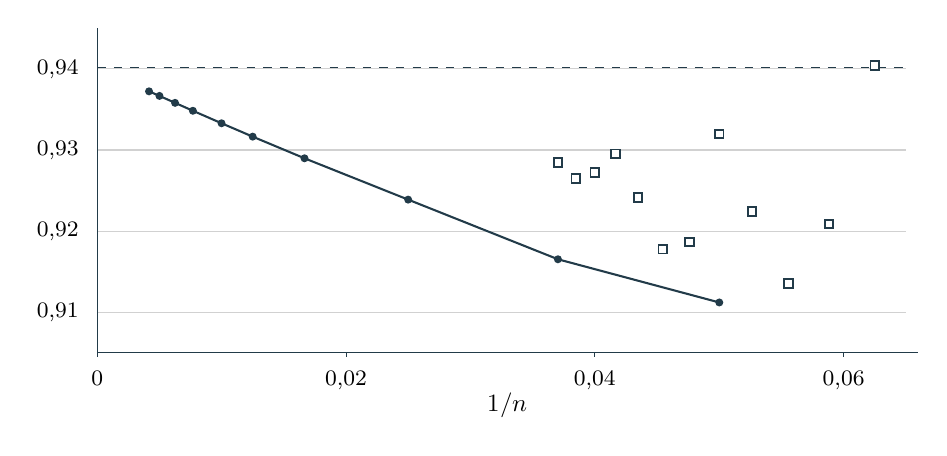
\begin{tikzpicture}[x=158cm,y=103cm]
 \begin{scope}[shift={(0,-.905)}]
 \foreach \v/\letra in {.910/{0,91},.920/{0,92},.930/{0,93},.940/{0,94}}{
   \draw[black!18] (0,\v)--(.065,\v);
   \node[anchor=east,font=\footnotesize] at (-.0007,\v) {\letra};}
 \draw[btinta] (0,.905)--(.066,.905) (0,.905)--(0,.945);
 \foreach \v/\letra in {0/{0},.02/{0,02},.04/{0,04},.06/{0,06}}{
   \draw[btinta] (\v,.905)--(\v,.9045);
   \node[anchor=north,font=\footnotesize] at (\v,.904) {\letra};}
 \draw[btinta,dashed] (0,.940144)--(.065,.940144);
 \draw[btinta,line width=.75pt] plot coordinates {(0.050000000,0.911188472) (0.037037037,0.916522978) (0.025000000,0.923873790) (0.016666667,0.928966033) (0.012500000,0.931643280) (0.010000000,0.933288384) (0.007692308,0.934831567) (0.006250000,0.935807595) (0.005000000,0.936660345) (0.004166667,0.937232189)};
 \foreach \x/\y in {0.050000000/0.911188472,0.037037037/0.916522978,0.025000000/0.923873790,0.016666667/0.928966033,0.012500000/0.931643280,0.010000000/0.933288384,0.007692308/0.934831567,0.006250000/0.935807595,0.005000000/0.936660345,0.004166667/0.937232189}{\fill[btinta] (\x,\y) circle[radius=1.45pt];}
 \foreach \x/\y in {0.062500000/0.940434608,0.058823529/0.920874442,0.055555556/0.913509083,0.052631579/0.922429638,0.050000000/0.931979175,0.047619048/0.918660405,0.045454545/0.917777869,0.043478261/0.924122583,0.041666667/0.929528249,0.040000000/0.927235036,0.038461538/0.926480702,0.037037037/0.928458576}{\draw[btinta,fill=white,line width=.65pt]
    (\x,\y) ++(-1.55pt,-1.55pt) rectangle ++(3.1pt,3.1pt);}
 \node[anchor=north,font=\small] at (.033,.9012) {$1/n$};
 \end{scope}
\end{tikzpicture}
\caption{Términos centrados con la misma referencia $\Phi_0$. Los círculos, unidos por segmentos,
representan el predictor de la Tabla~\ref{tab:predictor}; los cuadrados, sin unir, el conteo exacto
de la Tabla~\ref{tab:exacto}. La línea horizontal discontinua marca la evaluación de la constante
del predictor mediante la discretización de Nyström. Los tamaños representados son los de las dos tablas.}
\label{fig:comparacion}
\end{figure}


En $n=20$ y $n=27$ se tiene $\log Q(n)-\log Q_{\rm pred}(n)=0{,}0208$ y $0{,}0119$. Los dos números
son compatibles con una diferencia de orden $1/n$, pero no permiten estimar su límite.

Los programas y los datos con los que se obtuvieron las cifras de esta sección forman el paquete de
verificación numérica que acompaña al artículo~\cite{Codigo}.

\section{Discusión}\label{sec:discusion}

\paragraph{Lo que queda abierto para el conteo exacto.}
Pongamos $R_Q(n)=\log Q(n)-\log Q_{\rm pred}(n)$. El Teorema~\ref{thm:intro-constante} equivale a
\[
 \log Q(n)-\log n!-n\Phi=C_{\rm pred}+R_Q(n)+o(1).
\]
Por tanto, $R_Q(n)\to0$ basta para que el término constante de $\log Q(n)$ sea $C_{\rm pred}$. Si
sólo se supiera que $R_Q(n)$ tiene un límite finito $r$, el término constante existiría y valdría
$C_{\rm pred}+r$. No hemos probado ninguna de las dos afirmaciones. La forma cuantitativa natural
es la siguiente.

\begin{conjetura}\label{conj:RQ}
Existen $C$ y $n_0$ tales que $|\log Q(n)-\log Q_{\rm pred}(n)|\le C/n$ para todo $n\ge n_0$.
\end{conjetura}

La Sección~\ref{sec:numerico} da $R_Q(20)\approx0{,}021$ y $R_Q(27)\approx0{,}012$.

\paragraph{El papel de la consistencia.}
El Teorema~\ref{thm:intro-consistencia} dice que, en los residuales de sus clases, el predictor cumple
paso a paso la recursión exacta del conteo salvo un factor $e^{O(k^{-2})}$. A lo largo de una trayectoria de residuales que
permanezca en una misma clase con $k\ge\delta_0n$, los errores suman $O_{\delta_0}(1/n)$
(Sección~\ref{sec:B4T05}). Para pasar de ahí a $R_Q(n)\to0$ hacen falta tres piezas que este artículo
no contiene: que los residuales típicos de una colocación al azar estén en esas clases, el control del
final del proceso, cuando quedan pocas filas vacías (en~\cite{Completabilidad} se estudia, para el
conteo exacto, el caso de un número fijo de reinas por colocar, sin uniformidad cuando ese número
crece), y la comparación entre el conteo y el predictor a
lo largo de trayectorias aleatorias.

\paragraph{Actividad finita.}
El predictor se ha definido directamente en el tablero lleno, sobre el politopo $K_n$. Con una
actividad finita $\lambda$, la aproximación correspondiente usa la rama pequeña de las ecuaciones de
Bethe. Para $n\ge6$, que la rama pequeña exista para todo $\lambda>0$ es una conjetura. Un cálculo en
punto flotante, sin cotas rigurosas, la encuentra en las 61 actividades ensayadas, espaciadas
logarítmicamente entre $\Lambda=\lambda(n-1)=10^{-3}$ y $10^{12}$, para $n=6$, $7$, $8$, $10$, $12$,
$16$, $20$, $27$, $40$, $60$, $80$, $120$ y $160$. Para $n=4$, $K_4$ se reduce al punto
$\pi\equiv1/4$, porque cada fila tiene cuatro casillas con $p_c\le1/4$ y suma uno; por tanto
$(H_\infty)$ no se cumple. Para $n=5$, el cálculo indica $\max_c\pi^{(5)}_c=1/4$. En ambos casos, un
optimizador de barrera sugiere que la rama deja de existir para $\Lambda$ grande, pero no está
demostrado. Nada de lo expuesto en este párrafo se usa en el resto del artículo.

% El ancla del marcador va dentro del título, para que el marcador del PDF lleve al título.
\section*{\phantomsection Uso de herramientas de inteligencia artificial}
\addcontentsline{toc}{section}{Uso de herramientas de inteligencia artificial}

Se utilizaron herramientas de inteligencia artificial para organizar las fuentes, cotejar
versiones, preparar la composición y la reestructuración editorial del texto, y realizar revisiones
adversariales de extractos textuales.

\appendix
\section{Un caso modelo: las torres}\label{sec:torres}

En este apéndice estudiamos la construcción del predictor en el modelo de torres, en el que sólo hay
filas y columnas. Allí todo es explícito, y se puede probar que la fórmula de Bethe con la corrección de
un lazo y la normalización exacta del modo cero aproxima el logaritmo del conteo con error $O(1/k)$,
uniformemente desde densidades positivas hasta el tablero lleno. Ninguna prueba del resto del artículo
usa este apéndice, que tiene notación propia: aquí $p$ es la probabilidad de casilla de Bethe,
$\pi=3{,}14159\ldots$ y $D$ es una ley de probabilidad.

\subsection{Definiciones y enunciado}

\paragraph{El modelo.}
Sea $k\ge3$. En el tablero de $k\times k$, las líneas son las $k$ filas y las $k$ columnas. Para
$\lambda>0$ ponemos
\[
 Z_k(\lambda)=\sum_{q=0}^{k}\binom kq^2q!\,\lambda^q,
\]
que es la suma, sobre todas las colocaciones de torres que no se atacan, del peso $\lambda^q$, donde $q$
es el número de torres. Para obtener
el coeficiente se eligen primero las $q$ filas ocupadas y las $q$ columnas ocupadas; después, cada
biyección entre los dos conjuntos coloca una torre en cada fila elegida y da lugar a una de las $q!$
colocaciones posibles para esa elección. Escribimos $\Lambda=\lambda(k-1)$.

\paragraph{El punto fijo de Bethe uniforme.}
La probabilidad de casilla $p\in(0,1/k)$ y la probabilidad de línea vacía $y\in(0,1)$ cumplen
\begin{equation}\label{eq:torres-punto}
 p(1-p)=\lambda y^2,\qquad y=1-kp.
\end{equation}
Es la ecuación general $p_c(1-p_c)^{d-1}=\lambda\prod_{L\ni c}y_L$, con $y_L=1-\sum_{c\in L}p_c$
y $d$ el número de líneas que pasan por cada casilla, para $d=2$ y todas las variables iguales. Ponemos $\theta=1-y=kp$, la media de Bethe del número de torres por fila,
$w=p/(1-p)$ y $u=k\theta/(1-p)$.

\paragraph{Las tres piezas de la fórmula.}
En ese punto fijo definimos:
\begin{itemize}
\item el término de árbol
 \[
  \log Z_B=(\log\lambda)\sum_cp-\sum_Ly\log y-\sum_cp\log p+\sum_c(1-p)\log(1-p),
 \]
 donde $c$ recorre las $k^2$ casillas y $L$ las $2k$ líneas;
\item la matriz de un lazo $M$, que actúa sobre los $2k^2$ estados $(c,f)$, con
 $f\in\{\text{fila},\text{columna}\}$: $M[(c,f),(c',f')]=w$ si $f'\ne f$, $c'$ está en la línea de la
 familia $f'$ que pasa por $c$ y $c'\ne c$, y $M[(c,f),(c',f')]=0$ en otro caso;
\item el factor del modo cero $\rho_0=\mathsf P/P_G$, donde $\mathsf P=\mathbb P(N_R=N_C)$ para dos variables
 independientes $N_R$ y $N_C$ con ley $\mathrm{Bin}(k,y)$, que representan los números auxiliares de filas y
 columnas vacías en el modelo de Bethe, y $P_G=(2\pi(V_R+V_C))^{-1/2}$, con $V_R=V_C=ky(1-y)$.
\end{itemize}
La fórmula y su resto son
\begin{equation}\label{eq:torres-formula}
 F_k(\lambda)=\log Z_B-\tfrac12\log\det(I+M)+\log\rho_0,\qquad R'_k(\lambda)=\log Z_k(\lambda)-F_k(\lambda).
\end{equation}

\begin{teorema}[Modelo de torres]\label{thm:torres}
El resto $R'_k$ de~\eqref{eq:torres-formula} cumple lo siguiente.
\begin{enumerate}[(i)]
\item \emph{Cota uniforme.} Para cada $\Lambda_0>0$ existe una constante $C=C(\Lambda_0)$ tal que, para
 todo $k\ge3$ y todo $\lambda$ con $\Lambda=\lambda(k-1)\ge\Lambda_0$, se tiene $|R'_k(\lambda)|\le C/k$.
 Además, $R'_k(\lambda)$ tiene un límite $R'_k(\infty)$ cuando $\lambda\to\infty$, y la misma cota vale
 para él.
\item \emph{Tablero lleno.}
 \[
 \begin{aligned}
  R'_k(\infty)={}&\log k!-k\log k-k(k-1)\log\bigl(1-\tfrac1k\bigr)
  +\tfrac12(k-1)^2\log\bigl(1-(k-1)^{-2}\bigr)\\
  &+\tfrac12\log\frac{2k}{k-1}+(k-1)\log\frac k{k-1}-\tfrac12\log(4\pi k),
 \end{aligned}
 \]
 y $R'_k(\infty)=-\frac1{12k}-\frac1{4k^2}+O(k^{-3})$.
\item \emph{Hace falta $\Lambda_0>0$.} Para cada $k$ fijo, $R'_k(\lambda)=-\frac12\log(4\pi k^2\lambda)+o(1)$
 cuando $\lambda\to0^+$. En particular, $R'_k$ no está acotado en $\lambda\in(0,\infty)$.
\end{enumerate}
\end{teorema}

Los tres primeros términos de (ii) son $\log k!-\log\operatorname{perm}_B(J_k)$, donde $J_k$ es la matriz
$k\times k$ de unos y $\operatorname{perm}_B$ es el permanente de Bethe~\cite{Vontobel}.

\begin{observacion}[Por qué $k\ge3$]
Para $k=2$ coinciden los factores $1-(k-1)^2w^2$ y $(1-w^2)^{(k-1)^2}$ del Lema~\ref{lem:torres-lazo}, y
$\det(I+M)=(1-w^2)^2(1+w^2)^2$ se anula como $y^2$ cuando $y\to0$. Entonces
$-\frac12\log\det(I+M)\sim-\log y$ no se compensa con el $\frac12\log y$ de $\log\rho_0$, y $R'_2\to-\infty$
como $-\frac14\log\Lambda$. Para $k\ge3$ sólo el factor $1-(k-1)^2w^2$ se anula cuando $y\to0$, lo hace
como $y$, y la cancelación es exacta (Sección~\ref{sec:torres-i}).
\end{observacion}

\begin{observacion}[La constante $C(\Lambda_0)$]
Por (iii), para cada $k$ fijo, $\sup\{|R'_k(\lambda)|:\lambda(k-1)\ge\Lambda_0\}\to\infty$ cuando
$\Lambda_0\to0$, así que $C(\Lambda_0)$ tiende necesariamente a infinito cuando $\Lambda_0\to0$. La prueba de (i) da una
cota explícita sólo para $k\ge k_2(\Lambda_0)$, con $k_2$ muy grande; para $3\le k<k_2$ la cota sale de un
argumento de compacidad.
\end{observacion}

\paragraph{Idea de la prueba.}
Una identidad exacta (Lema~\ref{lem:torres-identidad}) escribe
$Z_k=Z_B\,(1-p)^{-k^2}\,\mathsf P\,\mathbb E_D[q!\,u^{-q}]$, donde $\mathbb E_D$ es un promedio sobre la ley
$D$ del número de filas ocupadas condicionada a $N_R=N_C$; el factor
$(1-p)^{-k^2}\approx e^{k\theta+\theta^2/2}$ no es despreciable. En el límite del tablero lleno se
tiene $\mathsf P\to1$ y $D$ se concentra en $q=k$. Tras dividir por $\lambda^k$, la identidad se
convierte en el caso de la matriz de unos de la fórmula de Watanabe y Chertkov~\cite{WC}, que expresa
el permanente de una matriz no negativa como el producto de su permanente de Bethe, del permanente de
la matriz de entradas $\beta_{ij}(1-\beta_{ij})$ y del factor $\prod_{i,j}(1-\beta_{ij})^{-1}$, donde
$\beta$ es la matriz doblemente estocástica del punto fijo de Bethe. Para la matriz de unos,
$\beta_{ij}=1/k$, y esos tres factores son los límites de $Z_B/\lambda^k$, de
$\mathbb E_D[q!\,u^{-q}]$ y de $(1-p)^{-k^2}$. El factor discreto $\mathsf P$, que es el
modo cero, se cancela exactamente con el de la fórmula. Queda el promedio $\mathbb E_D[q!\,u^{-q}]$ de una
función que varía despacio, y ese promedio se evalúa con el método de Laplace en una variable. Las cotas
necesarias salen de que $D$ es una ley de Poisson binomial, cuyos parámetros vienen de los ceros de los
polinomios de Legendre, y de la desigualdad de Bruns.

\subsection{El punto fijo uniforme y las formas cerradas}

\begin{lema}\label{lem:torres-punto}
Para cada $\lambda>0$ hay un único $y\in(0,1)$ que cumple~\eqref{eq:torres-punto}. La aplicación
$\lambda\mapsto y$ es una biyección continua y decreciente de $(0,\infty)$ en $(0,1)$, con $y\to0$ cuando
$\lambda\to\infty$ e $y\to1$ cuando $\lambda\to0$. Además $\Lambda\le\theta/y^2$; por tanto,
$\Lambda\ge\Lambda_0$ implica $\theta\ge\theta_0$, donde $\theta_0\in(0,1)$ es la raíz de
$\theta_0=\Lambda_0(1-\theta_0)^2$.
\end{lema}
\begin{proof}
Con $p=(1-y)/k$, la ecuación~\eqref{eq:torres-punto} dice $\lambda=\varphi(y)$, con
$\varphi(y)=(1-y)(k-1+y)/(k^2y^2)$. La función $\varphi$ es suave en $(0,1]$, tiende a $\infty$ cuando
$y\to0^+$ y vale $\varphi(1)=0$. Sea $\mathcal N(y)=(1-y)(k-1+y)=(k-1)-(k-2)y-y^2$. Entonces
$\varphi'(y)=(\mathcal N'(y)y-2\mathcal N(y))/(k^2y^3)$ y
\[
 \mathcal N'(y)y-2\mathcal N(y)=(k-2)y-2(k-1)<0\qquad\text{en }(0,1).
\]
Así $\varphi$ es estrictamente decreciente, lo que da la biyección y los límites. Para la cota,
\[
 \Lambda=(k-1)\varphi(y)=\frac{\theta}{y^2}\cdot\frac{k-1}k\cdot\frac{k-1+y}k\le\frac\theta{y^2}.
\]
Si $\Lambda\ge\Lambda_0$, entonces $\theta\ge\Lambda_0y^2=\Lambda_0(1-\theta)^2$. La función
$\theta\mapsto\theta-\Lambda_0(1-\theta)^2$ es creciente en $[0,1]$, de $-\Lambda_0$ a $1$; por tanto
$\theta\ge\theta_0$.
\end{proof}

\begin{lema}[Árbol]\label{lem:torres-arbol}
En el punto fijo uniforme, $\log Z_B=-2k\log y+k^2\log(1-p)$.
\end{lema}
\begin{proof}
Hay $k^2$ casillas y $2k$ líneas, y $\sum_cp=k^2p=k\theta$. Por tanto
\[
 \log Z_B=k\theta\log\lambda-2ky\log y-k^2p\log p+k^2(1-p)\log(1-p).
\]
Por~\eqref{eq:torres-punto}, $\log\lambda=\log p+\log(1-p)-2\log y$. Al sustituir, el término
$k\theta\log p$ se cancela con $-k^2p\log p$, y queda
$\log Z_B=-2k(\theta+y)\log y+(k\theta+k^2-k^2p)\log(1-p)$. Como $\theta+y=1$ y $k^2p=k\theta$, eso es
$-2k\log y+k^2\log(1-p)$.
\end{proof}

\begin{lema}[Un lazo]\label{lem:torres-lazo}
Se tiene
\[
 \det(I+M)=\bigl(1-(k-1)^2w^2\bigr)\bigl(1+(k-1)w^2\bigr)^{2(k-1)}\bigl(1-w^2\bigr)^{(k-1)^2}
\]
y $1-(k-1)^2w^2=y\,(1+(k-2)p)/(1-p)^2$. Para $k\ge3$, todos los factores son positivos cuando
$y\in(0,1)$.
\end{lema}
\begin{proof}
Ordenamos los estados en dos bloques, $(c,\text{fila})$ y $(c,\text{columna})$; dentro de cada bloque,
la casilla $c=(i,j)$ va en el orden de Kronecker, con $i$ por fuera y $j$ por dentro. Sea $J$ la matriz
$k\times k$ de unos. Desde $(c,\text{fila})$ la familia siguiente es la de las columnas: $c'=(i',j)$ con
$i'\ne i$. Eso da el bloque $wE$ de las filas a las columnas, con $E=(J-I)\otimes I$. Desde
$(c,\text{columna})$ se pasa a $c'=(i,j')$ con $j'\ne j$, lo que da el bloque $wE'$, con
$E'=I\otimes(J-I)$. Los bloques diagonales son nulos, porque $f'\ne f$. Así, por el complemento de Schur,
\[
 I+M=\begin{pmatrix}I&wE\\ wE'&I\end{pmatrix},\qquad \det(I+M)=\det(I-w^2E'E),
\]
y $E'E=(J-I)\otimes(J-I)$. La matriz $J-I$ es simétrica, con autovalores $k-1$ (una vez) y $-1$ ($k-1$
veces). Los autovalores del producto de Kronecker son los productos: $(k-1)^2$ (una vez), $-(k-1)$
($2(k-1)$ veces) y $1$ ($(k-1)^2$ veces). De ahí la fórmula. Para la segunda identidad,
\[
 1-(k-1)^2w^2=\frac{\bigl[(1-p)-(k-1)p\bigr]\bigl[(1-p)+(k-1)p\bigr]}{(1-p)^2}
 =\frac{(1-kp)(1+(k-2)p)}{(1-p)^2}.
\]
Para la positividad, $p=\theta/k\le1/k$, así que $w\le1/(k-1)\le\frac12$ si $k\ge3$. Por tanto
$1-w^2\ge\frac34$, y el primer factor es proporcional a $y>0$.
\end{proof}

\begin{lema}[Modo cero]\label{lem:torres-cero}
Sea $\beta(q)=\binom kq\theta^qy^{k-q}$, la ley $\mathrm{Bin}(k,\theta)$ del número de filas ocupadas.
Entonces $\mathsf P=\sum_{q=0}^k\beta(q)^2$ y $\log\rho_0=\log\mathsf P+\frac12\log(4\pi ky\theta)$.
\end{lema}
\begin{proof}
La igualdad $N_R=N_C$ equivale a $k-N_R=k-N_C$, y $k-N_R$ tiene ley $\mathrm{Bin}(k,\theta)$. Además
$V_R+V_C=2ky\theta$.
\end{proof}

\subsection{La identidad exacta}

\begin{lema}\label{lem:torres-identidad}
Para todo $\lambda>0$, con $y=y(\lambda)$,
\[
 Z_k(\lambda)=y^{-2k}\sum_{q=0}^k\beta(q)^2q!\,u^{-q}.
\]
Sea $D$ la ley de probabilidad $D(q)=\beta(q)^2/\mathsf P$ en $\{0,\dots,k\}$. Entonces
\begin{equation}\label{eq:torres-identidad}
 R'_k(\lambda)=\log\mathbb E_D[q!\,u^{-q}]-k^2\log(1-p)+\tfrac12\log\det(I+M)-\tfrac12\log(4\pi ky\theta).
\end{equation}
\end{lema}
\begin{proof}
Como $\binom kq^2=\beta(q)^2\theta^{-2q}y^{-2(k-q)}$, se tiene
$Z_k=y^{-2k}\sum_q\beta(q)^2q!\,(\lambda y^2/\theta^2)^q$. Por~\eqref{eq:torres-punto} y $p=\theta/k$,
$\lambda y^2/\theta^2=p(1-p)/\theta^2=(1-p)/(k\theta)=1/u$, lo que da la primera fórmula. Por tanto
$\log Z_k=-2k\log y+\log\mathsf P+\log\mathbb E_D[q!\,u^{-q}]$. Al restar $F_k$, escrito con los
Lemas~\ref{lem:torres-arbol} y~\ref{lem:torres-cero}, los términos $-2k\log y$ y $\log\mathsf P$ se
cancelan exactamente, y queda~\eqref{eq:torres-identidad}.
\end{proof}

Así, toda la parte discreta del modo cero, que es la probabilidad exacta de $N_R=N_C$, aparece igual en
$Z_k$ y en la fórmula. Lo que queda es el promedio bajo $D$ de $q!\,u^{-q}$, una función que varía
despacio: la segunda diferencia de su logaritmo es $\log((q+1)/q)$, del orden de $1/q$.

\subsection{La ley \texorpdfstring{$D$}{D} y sus momentos}

\begin{lema}[Legendre]\label{lem:torres-legendre}
Sean $\cos\alpha_1>\dots>\cos\alpha_k$ los ceros del polinomio de Legendre $P_k$, con
$0<\alpha_1<\dots<\alpha_k<\pi$. Entonces, para todo $x$,
\[
 f_k(x):=\sum_{q=0}^k\binom kq^2x^q=\prod_{i=1}^k(1+xc_i),\qquad c_i=\cot^2(\alpha_i/2)>0.
\]
\end{lema}
\begin{proof}
Por la fórmula de Rodrigues, $P_k(t)=(2^kk!)^{-1}(d/dt)^k[(t-1)^k(t+1)^k]$, y por la regla de Leibniz
\[
 \Bigl(\frac{d}{dt}\Bigr)^k\bigl[(t-1)^k(t+1)^k\bigr]
 =\sum_q\binom kq\frac{k!}{q!}(t-1)^q\,\frac{k!}{(k-q)!}(t+1)^{k-q}.
\]
Por tanto $P_k(t)=\sum_q\binom kq^2\bigl(\frac{t-1}2\bigr)^q\bigl(\frac{t+1}2\bigr)^{k-q}$. Para $x\ne1$, sea
$t=(1+x)/(1-x)$. Entonces $(t-1)/2=x/(1-x)$ y $(t+1)/2=1/(1-x)$, y queda
$f_k(x)=(1-x)^kP_k\bigl((1+x)/(1-x)\bigr)$; ambos lados son polinomios en $x$, así que la identidad vale
para todo $x$. El polinomio $P_k$ tiene $k$ ceros simples $t_i=\cos\alpha_i$ en $(-1,1)$~\cite[Teorema~3.3.1]{Szego}. Si
$\kappa_k$ es su coeficiente principal, $f_k(x)=\kappa_k\prod_i[(1-t_i)+x(1+t_i)]$. Como $f_k(0)=1$, se
tiene $\kappa_k\prod_i(1-t_i)=1$. Con $(1+\cos\alpha)/(1-\cos\alpha)=\cot^2(\alpha/2)$ se obtiene el producto
del enunciado.
\end{proof}

\begin{corolario}\label{cor:torres-pb}
Sea $x=(\theta/y)^2$, de modo que $D(q)=\binom kq^2x^q/f_k(x)$.
\begin{enumerate}[(a)]
\item La función generatriz es $\mathbb E_D[\tau^q]=f_k(x\tau)/f_k(x)=\prod_i(1-r_i+r_i\tau)$, con
 $r_i=xc_i/(1+xc_i)\in(0,1)$. Es decir, $D$ es la ley de una suma de $k$ variables de Bernoulli
 independientes de parámetros $r_i$.
\item Para $v\in\mathbb R$, la ley inclinada $D_v(q)\propto D(q)e^{vq}$ es de la misma familia, con $x$
 sustituido por $xe^v$.
\item La función $K(v)=\log\mathbb E_D[e^{vq}]=\sum_i\log(1-r_i+r_ie^v)$ cumple
 \[
 \begin{aligned}
  K'(v)&=\sum_ir_i(v)=:\mu(v),\qquad K''(v)=\sum_ir_i(v)(1-r_i(v))=:\sigma^2(v),\\
  K'''(v)&=\sum_ir_i(v)(1-r_i(v))(1-2r_i(v)),\\
  K''''(v)&=\sum_ir_i(v)(1-r_i(v))\bigl(1-6r_i(v)(1-r_i(v))\bigr),
 \end{aligned}
 \]
 con $r_i(v)=r_ie^v/(1-r_i+r_ie^v)$.
\item En consecuencia, $|K'''|\le K''$, $|K''''|\le K''$, $0\le K''\le k/4$,
 $K''(0)e^{-|v|}\le K''(v)\le K''(0)e^{|v|}$, y $K(v)\le0$ para $v\le0$.
\end{enumerate}
\end{corolario}
\begin{proof}
(a) sale del Lema~\ref{lem:torres-legendre}, y (b) de que $\binom kq^2(xe^v)^q\propto D(q)e^{vq}$. Las
derivadas de (c) son las de una suma de logaritmos de funciones generatrices de Bernoulli. Las
desigualdades $|1-2r|\le1$ y $|1-6r(1-r)|\le1$ dan las dos primeras cotas de (d), y $r(1-r)\le\frac14$ da
$K''\le k/4$. Para la cuarta basta $|(\log K'')'|=|K'''/K''|\le1$. Por último, $K(v)\le0$ para $v\le0$
porque $q\ge0$.
\end{proof}

\begin{lema}\label{lem:torres-momentos}
Sean $x>0$, $s=\sqrt x$, $\theta_x=s/(1+s)$ e $y_x=1-\theta_x$, y sean $\mu_D$ y $\sigma_D^2$ la media y la
varianza de la ley $q\mapsto\binom kq^2x^q/f_k(x)$. Entonces
\[
 \bigl|\mu_D-(k+\tfrac12)\theta_x\bigr|\le1,\qquad \bigl|\sigma_D^2-(k+\tfrac12)\theta_xy_x/2\bigr|\le1.
\]
Con $x=(\theta/y)^2$ la ley es $D$ y se tiene $\theta_x=\theta$ e $y_x=y$. Por el
Corolario~\ref{cor:torres-pb}(b), para la ley inclinada $D_v$, cuya media es $\mu(v)$ y cuya varianza es
$\sigma^2(v)$, basta poner $s_v=se^{v/2}$, $\theta_v=s_v/(1+s_v)$ e $y_v=1-\theta_v$.
\end{lema}
\begin{proof}
Por el Corolario~\ref{cor:torres-pb}, $\mu_D=\sum_iF(\alpha_i)$ y $\sigma_D^2=\sum_iG(\alpha_i)$, con
$F(\alpha)=s^2/(s^2+\tan^2(\alpha/2))$ y $G=F(1-F)$. La función $F$ es continua y decreciente en
$[0,\pi]$, de $1$ a $0$. La función $G$ toma valores en $[0,\frac14]$, se anula en los extremos y es
unimodal: crece mientras $F>\frac12$ y decrece mientras $F<\frac12$. Por la desigualdad de
Bruns~\cite{Bruns} (véase también~\cite[\S6.21]{Szego}), con $h=\pi/(k+\frac12)$,
\[
 (i-\tfrac12)h\le\alpha_i\le ih\qquad(i=1,\dots,k).
\]
Por el Lema~\ref{lem:torres-riemann}, que se prueba a continuación, con $m_0=1$ para $F$ y
$m_0=\frac14$ para $G$, cada suma difiere de $h^{-1}\int_0^\pi$ a lo sumo en $1$. Con $t=\tan(\alpha/2)$ y
$d\alpha=2\,dt/(1+t^2)$,
\[
\begin{aligned}
 \int_0^\pi F\,d\alpha&=2\int_0^\infty\frac{s^2\,dt}{(t^2+s^2)(1+t^2)}=\frac{\pi s}{1+s}=\pi\theta_x,\\
 \int_0^\pi G\,d\alpha&=2\int_0^\infty\frac{s^2t^2\,dt}{(t^2+s^2)^2(1+t^2)}=\frac{\pi s}{2(1+s)^2}
 =\frac\pi2\,\theta_xy_x;
\end{aligned}
\]
ambas salen por fracciones simples (en $s=1$, por continuidad). Como $h^{-1}=(k+\frac12)/\pi$, quedan
las cotas del enunciado.
\end{proof}

\begin{lema}[Sumas de Riemann en puntos entrelazados]\label{lem:torres-riemann}
Sean $h=\pi/(k+\frac12)$, $\alpha_i\in[(i-\frac12)h,ih]$ para $i=1,\dots,k$, y $m_0>0$.
\begin{enumerate}[(a)]
\item Si $F:[0,\pi]\to[0,m_0]$ es no creciente, entonces
 $\bigl|\sum_iF(\alpha_i)-h^{-1}\int_0^\pi F\bigr|\le m_0$.
\item Si $G:[0,\pi]\to[0,m_0]$ es unimodal, entonces
 $\bigl|\sum_iG(\alpha_i)-h^{-1}\int_0^\pi G\bigr|\le4m_0$.
\end{enumerate}
\end{lema}
\begin{proof}
(a) Extendemos $F$ por $0$ fuera de $[0,\pi]$; sigue siendo no creciente en $[0,\infty)$. Por un lado,
$F(\alpha_i)\le F((i-\frac12)h)$, que para $i\ge2$ es a lo sumo $h^{-1}\int_{(i-3/2)h}^{(i-1/2)h}F$ y para
$i=1$ es a lo sumo $m_0$; por tanto $\sum_iF(\alpha_i)\le m_0+h^{-1}\int_0^\pi F$. Por otro,
$F(\alpha_i)\ge F(ih)\ge h^{-1}\int_{ih}^{(i+1)h}F$; como $(k+1)h\ge\pi$, se tiene
$\sum_iF(\alpha_i)\ge h^{-1}\int_h^\pi F\ge h^{-1}\int_0^\pi F-m_0$.

(b) Ponemos $I_i=[(i-1)h,ih]$. Como $\alpha_i\in I_i$,
\[
 \left|G(\alpha_i)-h^{-1}\int_{I_i}G\right|
 \le\operatorname{osc}_{I_i}G .
\]
Por unimodalidad y $0\le G\le m_0$, la suma de las oscilaciones en estos intervalos
es a lo sumo la variación total de $G$ en $[0,kh]$, que es a lo sumo $2m_0$.
Como $\pi-kh=h/2$, el resto $h^{-1}\int_{kh}^{\pi}G$ aporta a lo sumo $m_0/2$.
La desigualdad triangular da la cota $5m_0/2\le4m_0$, también cuando la moda está en un extremo.
\end{proof}

\subsection{El paso de Laplace}

Como $q!=\int_0^\infty e^{-t}t^q\,dt$, por el teorema de Tonelli
$\mathbb E_D[q!\,u^{-q}]=\int_0^\infty e^{-t}\,\mathbb E_D[(t/u)^q]\,dt$. Con $t=ue^v$ queda
\begin{equation}\label{eq:torres-laplace}
 \mathbb E_D[q!\,u^{-q}]=u\int_{\mathbb R}e^{\Psi(v)}\,dv,\qquad \Psi(v)=-ue^v+v+K(v),
\end{equation}
con $\Psi(0)=-u$, $\Psi'(0)=1+\mu_D-u$ y $\Psi''(0)=-(u-\sigma_D^2)$.

\begin{lema}\label{lem:torres-psi}
Supongamos $\theta\in[\theta_0,1)$, es decir, $\lambda<\infty$, de modo que $x=(\theta/y)^2$ es finito, y
$k\ge k_1:=\max(11,20/\theta_0)$. Sea $\delta=0{,}3$. Entonces:
\begin{enumerate}[(a)]
\item $\Psi''(v)\le-a$ para todo $v\ge-\delta$, con $a=0{,}08\,k\theta_0$;
\item $\Psi'(v)>0$ para todo $v\le-\delta$, y $\Psi(v)\le v$ para todo $v\le0$;
\item $|\Psi'''(v)|\le b$ y $|\Psi''''(v)|\le b$ para $|v|\le\delta$, con $b=2k$;
\item $|\Psi'(0)|\le4{,}5$ y $k\theta(1+\theta)/2-3{,}1\le u-\sigma_D^2\le k\theta(1+\theta)/2+3{,}1$.
\end{enumerate}
\end{lema}
\begin{proof}
(a) Se tiene $\Psi''(v)=-ue^v+\sigma^2(v)$ y, por el Lema~\ref{lem:torres-momentos} aplicado a $D_v$,
$\sigma^2(v)\le(k+\frac12)\theta_vy_v/2+1$, con $\theta_vy_v=s_v/(1+s_v)^2$. Como $u\ge k\theta=ks/(1+s)$,
\[
 -\Psi''(v)\ge k\,se^{v/2}\Bigl[\frac{e^{v/2}}{1+s}-\frac1{2(1+se^{v/2})^2}\Bigr]-\frac1{16}-1.
\]
Para $v\ge-\delta$, $1+se^{v/2}\ge e^{-\delta/2}(1+s)$, así que el corchete es al menos
$(e^{-\delta/2}-e^\delta/2)/(1+s)>\gamma/(1+s)$, con $\gamma=0{,}1857$. Por tanto
$-\Psi''(v)\ge\gamma e^{-\delta/2}k\theta-1{,}07\ge0{,}159\,k\theta-1{,}07\ge0{,}08\,k\theta_0$ si
$k\theta_0\ge14$.

(b) Por el Lema~\ref{lem:torres-momentos}, $\Psi'(v)=-ue^v+1+\mu(v)\ge(k+\frac12)\theta_v-ue^v$. Para
$v\le0$, $\theta_v\ge se^{v/2}/(1+s)=\theta e^{v/2}$ y $u\le k\theta/(1-1/k)$. Por tanto
$\Psi'(v)\ge k\theta e^{v/2}\bigl[1-e^{v/2}/(1-1/k)\bigr]>0$ para $v\le-\delta$, porque
$e^{-\delta/2}<0{,}861<1-1/k$ cuando $k\ge8$. Además $\Psi(v)\le v$ para $v\le0$, porque $-ue^v<0$ y
$K(v)\le0$.

(c) Se tiene $\Psi'''=-ue^v+K'''$ y $\Psi''''=-ue^v+K''''$. Como $|K'''|,|K''''|\le k/4$ y
$ue^v\le1{,}1k\,e^{0{,}3}\le1{,}5k$ para $k\ge11$, ambas son a lo sumo $1{,}75k\le b$.

(d) Por el Lema~\ref{lem:torres-momentos}, $|\mu_D-k\theta|\le1+\theta/2\le\frac32$, y
$u-k\theta=\theta^2/(1-p)\in[0,2]$; como $\Psi'(0)=1+(\mu_D-k\theta)-(u-k\theta)$, resulta
$|\Psi'(0)|\le4{,}5$. Para $u-\sigma_D^2$ se usan además $|\sigma_D^2-(k+\frac12)\theta y/2|\le1$ y
$1-y/2=(1+\theta)/2$.
\end{proof}

\begin{lema}[Laplace con error explícito]\label{lem:torres-laplace}
Sean $\Psi\in C^4(\mathbb R)$ y constantes $a,b>0$, $\delta\in(0,1]$, $r\in(0,\delta/2]$ con $r\le1$ y
$br\le a$, y $V\ge0$, tales que:
\begin{enumerate}[label=(L\arabic*)]
\item $\Psi''\le-a$ en $[-\delta,\infty)$;
\item $\Psi'>0$ en $(-\infty,-\delta]$, y $\Psi(v)\le v$ para $v\le-\delta$;
\item $|\Psi'''|\le b$ y $|\Psi''''|\le b$ en $[-\delta,\delta]$;
\item existe $v^*$ con $|v^*|\le\delta/2$ y $\Psi'(v^*)=0$;
\item $\Psi(v^*)\ge-V$.
\end{enumerate}
Entonces $v^*$ es el máximo global de $\Psi$ y, con $A=-\Psi''(v^*)\ge a$,
$\int_{\mathbb R}e^{\Psi}=e^{\Psi(v^*)}\sqrt{2\pi/A}\,(1+\varepsilon)$, donde
\[
 |\varepsilon|\le\frac b{8A^2}+\frac{6b^2}{A^3}+\frac{e^{-Ar^2/2}}{r\sqrt A}
 +\sqrt A\Bigl[\frac{2e^{-ar^2/2}}{ar}+\Bigl(1+V+\frac{a\delta^2}8\Bigr)e^{-a\delta^2/8}\Bigr].
\]
\end{lema}
\begin{proof}
\emph{Máximo global.} Por (L1) y (L2), $\Psi$ crece en $(-\infty,-\delta]$ y es estrictamente cóncava en
$[-\delta,\infty)$, así que $v^*$ es el máximo global.

\emph{Centro, $|t|\le r$, con $t=v-v^*$.} Por Taylor, $\Psi(v^*+t)=\Psi(v^*)-At^2/2+S(t)$, con
$S(t)=\Psi'''(v^*)t^3/6+T(t)$ y $|T(t)|\le bt^4/24$. Como $|t|\le r\le1$,
$|S|\le b|t|^3/4\le(br/4)t^2\le(A/4)t^2$. Escribimos $e^S=1+S+R_2$, con $|R_2|\le S^2e^{|S|}/2$. El término
cúbico integra cero en $[-r,r]$, y
\[
 \Bigl|\int e^{-At^2/2}\,T\Bigr|\le\frac b{24}\,3\sqrt{2\pi}\,A^{-5/2}=\sqrt{\frac{2\pi}A}\,\frac b{8A^2},
\]
\[
 \Bigl|\int e^{-At^2/2}R_2\Bigr|\le\frac{b^2}{32}\int t^6e^{-At^2/4}\,dt
 =\sqrt{\frac{2\pi}A}\,\frac{15\cdot2^{7/2}}{32}\,\frac{b^2}{A^3}\le\sqrt{\frac{2\pi}A}\,\frac{6b^2}{A^3}.
\]
Truncar la gaussiana en $|t|>r$ cuesta a lo sumo $2e^{-Ar^2/2}/(Ar)$, es decir, un error relativo a lo
sumo $e^{-Ar^2/2}/(r\sqrt A)$.

\emph{Laterales en $[-\delta,\infty)$ fuera del centro.} Por concavidad (L1), para $v\ge v^*+r$,
$\Psi(v)\le\Psi(v^*)-ar^2/2-ar(v-v^*-r)$, y lo análogo vale en $[-\delta,v^*-r]$. Su contribución es a lo
sumo $2e^{\Psi(v^*)-ar^2/2}/(ar)$.

\emph{Cola $(-\infty,-\delta]$.} Sea $V'=V+a\delta^2/8$. Si $V'<\delta$, no hace falta partir la integral:
por (L2), $\int_{-\infty}^{-\delta}e^\Psi\le\int_{-\infty}^{-\delta}e^v\,dv=e^{-\delta}\le e^{-V'}$.
Supongamos ahora $V'\ge\delta$, que es lo que ocurre en la Proposición~\ref{prop:torres-laplace}, donde
$V'\ge u\ge k\theta_0>375$. Por (L2) y (L5), $\int_{-\infty}^{-V'}e^\Psi\le e^{-V'}\le e^{\Psi(v^*)-a\delta^2/8}$.
Como $\Psi$ es creciente en $[-V',-\delta]$, $\int_{-V'}^{-\delta}e^\Psi\le V'e^{\Psi(-\delta)}$, y por
concavidad y $|v^*|\le\delta/2$, $\Psi(-\delta)\le\Psi(v^*)-a\delta^2/8$.

Dividiendo por $e^{\Psi(v^*)}\sqrt{2\pi/A}$ y usando $(2\pi)^{-1/2}\le1$ se obtiene la cota.
\end{proof}

\begin{proposicion}\label{prop:torres-laplace}
Para cada $\theta_0\in(0,1]$ existen $k_2(\theta_0)$ y $C_1(\theta_0)$ tales que, si $\theta\in[\theta_0,1)$ y
$k\ge k_2$,
\[
 \log\mathbb E_D[q!\,u^{-q}]=\log u-u+\tfrac12\log(2\pi)-\tfrac12\log(u-\sigma_D^2)+\varepsilon',\qquad
 |\varepsilon'|\le C_1/k.
\]
\end{proposicion}
\begin{proof}
\emph{Hipótesis del Lema~\ref{lem:torres-laplace}.} Tomamos $\delta=0{,}3$, $a=0{,}08\,k\theta_0$, $b=2k$,
$r=a/b=0{,}04\,\theta_0$ y $V=u$. Las hipótesis (L1)--(L3) se cumplen por el Lema~\ref{lem:torres-psi}, y
(L5) vale porque $\Psi(v^*)\ge\Psi(0)=-u$. En cuanto a (L4), $\Psi'$ es estrictamente decreciente en
$[-\delta,\infty)$, con pendiente a lo sumo $-a$; por tanto $\Psi'(\delta/2)\le\Psi'(0)-a\delta/2$ y
$\Psi'(-\delta/2)\ge\Psi'(0)+a\delta/2$. Como $|\Psi'(0)|\le4{,}5<a\delta/2$ si $k\theta_0>375$, el primero
es negativo y el segundo positivo. Hay entonces un único $v^*$ con $\Psi'(v^*)=0$, y
$|v^*|\le|\Psi'(0)|/a\le4{,}5/a\le\delta/2$.

\emph{Tamaño del error.} Como $K''\ge0$ y $|v^*|\le\delta/2$,
$A=ue^{v^*}-K''(v^*)\le ue^{\delta/2}\le1{,}1\,e^{0{,}15}k\le1{,}28k$; junto con $A\ge a$, se tiene
$a\le A\le1{,}28k$. Los dos primeros términos de la cota de $|\varepsilon|$ son $O(1/k)$:
$b/(8A^2)\le2k/(8a^2)$ y $6b^2/A^3\le6b^2/a^3=46875/(\theta_0^3k)$. Con $\theta_0$ fijo, $r$ es constante,
$V=O(k)$ y $A$ es de orden $k$; por tanto, los términos de cola son
$O_{\theta_0}(k^{3/2}e^{-c(\theta_0)k})$, con $c(\theta_0)>0$. Tomando $0<c'<c(\theta_0)$ se absorbe el
prefactor en $O_{\theta_0}(e^{-c'k})$. Al sumar los dos términos algebraicos y las colas se ve que existe
$k_2(\theta_0)$ tal que $|\varepsilon|\le1/2$ para $k\ge k_2$. Entonces
$|\log(1+\varepsilon)|\le2|\varepsilon|$.

\emph{Valor en el máximo.} Por Taylor en $0$ con $\Psi''\le-a$,
$\Psi(v^*)\le\Psi(0)+\Psi'(0)v^*-av^{*2}/2\le\Psi(0)+\Psi'(0)^2/(2a)$. Por tanto
$0\le\Psi(v^*)-\Psi(0)\le\Psi'(0)^2/(2a)\le10{,}2/a=O(1/k)$.

\emph{Curvatura.} Como $A=ue^{v^*}-K''(v^*)$,
\[
 |A-(u-\sigma_D^2)|\le ue^{\delta}|v^*|+\sigma_D^2\bigl(e^{|v^*|}-1\bigr)\le1{,}35\,(u+\sigma_D^2)\cdot4{,}5/a=O(1),
\]
porque $u+\sigma_D^2\le1{,}35k$. Como $u-\sigma_D^2\ge k\theta_0/2-3{,}1$, se tiene
$|\log A-\log(u-\sigma_D^2)|=O(1/k)$.

\emph{Conclusión.} Por~\eqref{eq:torres-laplace},
$\log\mathbb E_D[q!\,u^{-q}]=\log u+\Psi(v^*)+\frac12\log(2\pi/A)+\log(1+\varepsilon)$, de donde sale el
enunciado.
\end{proof}

El umbral $k\ge93750/\theta_0^3$ hace que $46875/(\theta_0^3k)\le1/2$; para acotar $|\varepsilon|$ por $1/2$
se elige $k_2$ considerando la suma completa. La constante $C(\Lambda_0)$ del Teorema~\ref{thm:torres}(i)
se obtiene además con un argumento de compacidad para $3\le k<k_2$.

\subsection{Prueba del Teorema~\ref{thm:torres}}\label{sec:torres-i}

\paragraph{Parte (i).}
Sea $\Lambda_0\le\Lambda<\infty$, de modo que $\theta\in[\theta_0,1)$ por el Lema~\ref{lem:torres-punto}; el
caso $\lambda=\infty$ se trata al final por paso al límite. Sustituimos en~\eqref{eq:torres-identidad} la
Proposición~\ref{prop:torres-laplace} y el Lema~\ref{lem:torres-lazo}. El término $\frac12\log y$ del
Lema~\ref{lem:torres-lazo} se cancela con el $-\frac12\log y$ de $-\frac12\log(4\pi ky\theta)$: es la
cancelación del modo cero. Usando además $\log u=\log(k\theta)-\log(1-p)$ y el
Lema~\ref{lem:torres-psi}(d) para $\log(u-\sigma_D^2)=\log(k\theta(1+\theta)/2)+O(1/k)$, queda
\[
\begin{aligned}
 R'_k={}&-u-2\log(1-p)-k^2\log(1-p)-\tfrac12\log(1+\theta)+\tfrac12(k-1)^2\log(1-w^2)\\
 &+\tfrac12\log(1+(k-2)p)+(k-1)\log(1+(k-1)w^2)+O(1/k).
\end{aligned}
\]
Hacemos los desarrollos con $p=\theta/k\le1/k$, $w\le1/(k-1)\le\frac12$ y $k\ge3$; todas las cotas son
uniformes en $\theta\in[0,1]$.
\begin{enumerate}[(a)]
\item $-k^2\log(1-p)=k\theta+\theta^2/2+e_1$, con $0\le e_1\le\frac23k^2p^3\le\frac2{3k}$.
\item $-u=-k\theta-\theta^2/(1-p)=-k\theta-\theta^2-e_2$, con $0\le e_2=\theta^2p/(1-p)\le2/k$.
\item $0\le-2\log(1-p)\le2p/(1-p)\le4/k$.
\item $\frac12(k-1)^2\log(1-w^2)=-\theta^2/2+e_4$, con $|e_4|\le2/k$. En efecto, si
 $\zeta=(1-1/k)/(1-\theta/k)\in[1-1/k,1]$, entonces $(k-1)^2w^2=\theta^2\zeta^2$ y
 $|\theta^2\zeta^2-\theta^2|\le2/k$; además $0\le-\log(1-w^2)-w^2\le\frac43w^4$ y $(k-1)^2w^4\le(k-1)^{-2}$.
\item $1+(k-2)p=1+\theta-2\theta/k$, y
 $\bigl|\frac12\log(1+\theta-2\theta/k)-\frac12\log(1+\theta)\bigr|\le\theta/k\le1/k$.
\item $(k-1)\log(1+(k-1)w^2)=\theta^2+e_6$, con $|e_6|\le3/k$; se usa $0\le z-\log(1+z)\le z^2/2$ con
 $z=(k-1)w^2\le1/(k-1)$, y lo mismo que en (d).
\end{enumerate}
Al sumar, los términos de orden $k$ se cancelan ($k\theta-k\theta$) y los de orden uno también:
\[
 -\theta^2+\tfrac12\theta^2-\tfrac12\log(1+\theta)-\tfrac12\theta^2+\tfrac12\log(1+\theta)+\theta^2=0.
\]
Por tanto $|R'_k|\le C(\theta_0)/k$ para $k\ge k_2(\theta_0)$.

Para $3\le k<k_2$, $R'_k$ es continua en $\lambda\in[\Lambda_0/(k-1),\infty)$, porque todas las piezas son
funciones continuas de $y\in(0,1)$ y $\lambda\mapsto y$ es continua, y tiene límite finito cuando
$\lambda\to\infty$ (véase el párrafo siguiente; es finito porque $k\ge3$). Por tanto está acotada, y como
sólo hay un número finito de esos $k$, basta tomar $C\ge\max_{3\le k<k_2}k\sup|R'_k|$.

En el límite $\lambda\to\infty$, el único término de~\eqref{eq:torres-identidad} que es singular cuando
$y\to0$ es $\frac12\log y$, y se cancela idénticamente. Los demás términos son continuos hasta $y=0$, donde $D$ es la
masa unidad en $q=k$. La cota uniforme pasa al límite.

\paragraph{Parte (ii).}
Cuando $\lambda\to\infty$ se tiene $y\to0$, $\theta\to1$, $p\to1/k$, $w\to1/(k-1)$ y $u\to k^2/(k-1)$, y $D$
tiende a la masa unidad en $q=k$, porque $r_i\to1$ cuando $x\to\infty$. En~\eqref{eq:torres-identidad}, con
la cancelación del $\frac12\log y$, queda
\[
\begin{aligned}
 R'_k(\infty)={}&\log k!-k\log\frac{k^2}{k-1}-k^2\log\bigl(1-\tfrac1k\bigr)
 +\tfrac12(k-1)^2\log\bigl(1-(k-1)^{-2}\bigr)\\
 &+\tfrac12\log\Bigl(1+\frac{k-2}k\Bigr)-\log\bigl(1-\tfrac1k\bigr)
 +(k-1)\log\Bigl(1+\frac1{k-1}\Bigr)-\tfrac12\log(4\pi k).
\end{aligned}
\]
Como $-k\log(k^2/(k-1))-k^2\log(1-1/k)=-k\log k-k(k-1)\log(1-1/k)$ y
$\frac12\log((2k-2)/k)-\log((k-1)/k)=\frac12\log(2k/(k-1))$, se obtiene la expresión del enunciado. Para el
desarrollo usamos la fórmula de Stirling, que no tiene término en $k^{-2}$, y los desarrollos siguientes:
\[
\begin{aligned}
 \log k!&=k\log k-k+\tfrac12\log(2\pi k)+\tfrac1{12k}+O(k^{-3}),\\
 -k(k-1)\log\bigl(1-\tfrac1k\bigr)&=(k-1)\sum_{m\ge1}\frac1{m\,k^{m-1}}
 =k-\tfrac12-\tfrac1{6k}-\tfrac1{12k^2}+O(k^{-3}),\\
 \tfrac12(k-1)^2\log\bigl(1-(k-1)^{-2}\bigr)&=-\tfrac12-\tfrac1{4(k-1)^2}+O(k^{-4})
 =-\tfrac12-\tfrac1{4k^2}+O(k^{-3}),\\
 \tfrac12\log\frac{2k}{k-1}&=\tfrac12\log2+\tfrac1{2k}+\tfrac1{4k^2}+O(k^{-3}),\\
 (k-1)\log\frac k{k-1}&=1-\tfrac1{2k}-\tfrac1{6k^2}+O(k^{-3}).
\end{aligned}
\]
Al sumar, $\frac12\log(2\pi k)+\frac12\log2-\frac12\log(4\pi k)=0$ y $-\frac12-\frac12+1=0$; el coeficiente
de $1/k$ es $\frac1{12}-\frac16+\frac12-\frac12=-\frac1{12}$, y el de $1/k^2$ es
$-\frac1{12}-\frac14+\frac14-\frac16=-\frac14$. Por tanto
$R'_k(\infty)=-\frac1{12k}-\frac1{4k^2}+O(k^{-3})$.

\paragraph{Parte (iii).}
Con $k$ fijo y $\lambda\to0^+$, se tiene $y\to1$ y $\theta\to0$. Por~\eqref{eq:torres-punto},
$p/\lambda\to1$, así que $\theta=kp\sim k\lambda$. Entonces $\log Z_k\to0$; además
$\log Z_B=-2k\log y+k^2\log(1-p)\to0$, $\det(I+M)\to1$ y $\mathsf P\to1$, porque el término $q=0$ de
$\sum_q\beta(q)^2$ es $y^{2k}\to1$. En cambio,
$\frac12\log(4\pi ky\theta)=\frac12\log(4\pi k^2\lambda)+o(1)\to-\infty$. Por tanto
$R'_k=-\frac12\log(4\pi k^2\lambda)+o(1)$.

\begin{observacion}[Lectura]
Cuando casi no hay torres, la gaussiana $P_G$ del balance $N_R-N_C$ es muy estrecha, porque su varianza
$2ky\theta$ tiende a cero, pero el determinante no tiene ahí ningún factor pequeño que la compense: el
factor del modo cero sobrecorrige. En el lado denso, en cambio, el factor de $\det(I+M)$ que tiende a cero
es proporcional a $y$ (Lema~\ref{lem:torres-lazo}) y se cancela con la varianza.

El argumento usa que el número de emparejamientos perfectos entre $q$ filas ocupadas y $q$ columnas
ocupadas es $q!$, lo que hace explícito el promedio del Lema~\ref{lem:torres-identidad}. En las reinas, el
factor correspondiente es el número de colocaciones que además respetan las diagonales, y contarlas es el
problema entero; por eso el argumento de este apéndice no se traslada a las reinas.
\end{observacion}


\begin{thebibliography}{99}
\addcontentsline{toc}{section}{Referencias}
\raggedright

\bibitem{Bass} H.~Bass, \emph{The Ihara--Selberg zeta function of a tree lattice}, Internat. J.
Math. \textbf{3} (1992), 717--797.
\href{https://doi.org/10.1142/S0129167X92000357}{doi:10.1142/S0129167X92000357}.

\bibitem{Bornemann} F.~Bornemann, \emph{On the numerical evaluation of Fredholm determinants}, Math.
Comp. \textbf{79} (2010), 871--915.
\href{https://doi.org/10.1090/S0025-5718-09-02280-7}{doi:10.1090/S0025-5718-09-02280-7}.

\bibitem{BK} C.~Bowtell y P.~Keevash, \emph{The $n$-queens problem}, arXiv:2109.08083v1 (2021).
\href{https://doi.org/10.48550/arXiv.2109.08083}{doi:10.48550/arXiv.2109.08083}.

\bibitem{Bruns} H.~Bruns, \emph{Zur Theorie der Kugelfunctionen}, J. Reine Angew. Math. \textbf{90}
(1881), 322--328.
\href{https://doi.org/10.1515/crll.1881.90.322}{doi:10.1515/crll.1881.90.322}.

\bibitem{Cherepanov} S.~Cherepanov, \emph{ColorSplit: counting $n$-queens solutions by splitting the
board into colors}, prepublicación, Zenodo, 2026, versión~1.
\href{https://doi.org/10.5281/zenodo.23901120}{doi:10.5281/zenodo.23901120}.

\bibitem{CC} M.~Chertkov y V.~Y.~Chernyak, \emph{Loop series for discrete statistical models on
graphs}, J. Stat. Mech. Theory Exp. (2006), P06009.
\href{https://doi.org/10.1088/1742-5468/2006/06/P06009}{doi:10.1088/1742-5468/2006/06/P06009}.

\bibitem{EMM19} S.~Eberhard, F.~Manners y R.~Mrazović, \emph{Additive triples of bijections, or the
toroidal semiqueens problem}, J. Eur. Math. Soc. \textbf{21} (2019), 441--463.
\href{https://doi.org/10.4171/JEMS/841}{doi:10.4171/JEMS/841}; arXiv:1510.05987.

\bibitem{EMM} S.~Eberhard, F.~Manners y R.~Mrazović, \emph{Transversals in quasirandom latin squares},
Proc. London Math. Soc. \textbf{127} (2023), 84--115.
\href{https://doi.org/10.1112/plms.12538}{doi:10.1112/plms.12538};
arXiv:2209.02180.

\bibitem{LLW} Z.-Y.~Liu, H.-J.~Liao y L.~Wang, \emph{Statistical mechanics of the $N$-queens problem},
Phys. Rev. E \textbf{114} (2026), 034125.
\href{https://doi.org/10.1103/cx7m-n3d5}{doi:10.1103/cx7m-n3d5}; arXiv:2605.10326.

\bibitem{LS} Z.~Luria y M.~Simkin, \emph{A lower bound for the $n$-queens problem}, en
\emph{Proceedings of the 2022 Annual ACM-SIAM Symposium on Discrete Algorithms (SODA)}, SIAM, 2022,
2185--2197.
\href{https://doi.org/10.1137/1.9781611977073.86}{doi:10.1137/1.9781611977073.86};
arXiv:2105.11431.

\bibitem{Completabilidad} D.~S.~Mejia, \emph{Completabilidad de las últimas capas en el problema de
las $n$ reinas}, prepublicación, Zenodo, 2026, versión~1.
\href{https://doi.org/10.5281/zenodo.24221374}{doi:10.5281/zenodo.24221374}.

\bibitem{Perfil} D.~S.~Mejia, \emph{El perfil variacional de las colocaciones parciales de reinas:
existencia, ecuaciones de Euler y regularidad hasta el tablero lleno}, prepublicación, Zenodo, 2026, versión~1.
\href{https://doi.org/10.5281/zenodo.24220042}{doi:10.5281/zenodo.24220042}.

\ifx\DOIcodigo\empty\else
\bibitem{Codigo} D.~S.~Mejia, \emph{Verificación numérica del predictor canónico del problema de las
$n$ reinas}, versión~2.1.0, 2026. \href{https://doi.org/\DOIcodigo}{doi:\DOIcodigo}.
\fi

\bibitem{NAB} P.~Nobel, A.~Agrawal y S.~Boyd, \emph{Computing tighter bounds on the $n$-queens
constant via Newton's method}, Optim. Lett. \textbf{17} (2023), 1229--1240.
\href{https://doi.org/10.1007/s11590-022-01933-2}{doi:10.1007/s11590-022-01933-2}.

\bibitem{OEIS} OEIS Foundation Inc., \emph{The On-Line Encyclopedia of Integer Sequences},
sucesión A000170. \url{https://oeis.org/A000170} (consultada el 15 de noviembre de 2026).

\bibitem{PE} T.~B.~Preußer y M.~R.~Engelhardt, \emph{Putting queens in carry chains, No.~27}, J. Signal
Process. Syst. \textbf{88} (2017), 185--201.
\href{https://doi.org/10.1007/s11265-016-1176-8}{doi:10.1007/s11265-016-1176-8}.

\bibitem{Simkin} M.~Simkin, \emph{The number of $n$-queens configurations}, Adv. Math.
\textbf{427} (2023), 109127.
\href{https://doi.org/10.1016/j.aim.2023.109127}{doi:10.1016/j.aim.2023.109127}. Citamos la numeración de
la versión arXiv:2107.13460v3.

\bibitem{Simon} B.~Simon, \emph{Trace Ideals and Their Applications}, 2.ª ed., Mathematical Surveys
and Monographs \textbf{120}, American Mathematical Society, 2005.

\bibitem{Szego} G.~Szegő, \emph{Orthogonal Polynomials}, 4.ª ed., American Mathematical Society Colloquium
Publications \textbf{23}, American Mathematical Society, 1975.

\bibitem{Vontobel} P.~O.~Vontobel, \emph{The Bethe permanent of a nonnegative matrix}, IEEE Trans.
Inform. Theory \textbf{59} (2013), 1866--1901.
\href{https://doi.org/10.1109/TIT.2012.2227109}{doi:10.1109/TIT.2012.2227109}.

\bibitem{WC} Y.~Watanabe y M.~Chertkov, \emph{Belief propagation and loop calculus for the permanent of a
non-negative matrix}, J. Phys. A: Math. Theor. \textbf{43} (2010), 242002.
\href{https://doi.org/10.1088/1751-8113/43/24/242002}{doi:10.1088/1751-8113/43/24/242002}; arXiv:0911.1419.

\bibitem{WF} Y.~Watanabe y K.~Fukumizu, \emph{Graph zeta function in the Bethe free energy and loopy
belief propagation}, en \emph{Advances in Neural Information Processing Systems 22}, 2009. arXiv:1002.3307.

\bibitem{YFW} J.~S.~Yedidia, W.~T.~Freeman e Y.~Weiss, \emph{Constructing free-energy approximations and
generalized belief propagation algorithms}, IEEE Trans. Inform. Theory \textbf{51} (2005), 2282--2312.
\href{https://doi.org/10.1109/TIT.2005.850085}{doi:10.1109/TIT.2005.850085}.

\end{thebibliography}

\end{document}
